\section{Subrings of Fields}
In this section we shall introduce some basic concepts in algebra and number theory. The reader is assumed to have a solid background of commutative algebra.
\subsection{Discrete Valuation Rings and Dedekind Rings}
In this section we give a brief review of discrete valuation rings and Dedekind rings. We first give the definitions.
\begin{definition}
A ring is called a \textit{discrete valuation ring} (DVR) if it is a principal ideal domain with only one maximal ideal.
\end{definition}
Trivially every field is a DVR. However we are mostly interested in the case that $R$ is a DVR but not a field. Some basic properties of a DVR is listed below:
\begin{proposition}
Let $R$ be a DVR and let $\pi\in R$ such that $\mathfrak{P}=R\pi$ is the unique maximal ideal.
\begin{enumerate}
    \item $R$ is a noetherian ring.
    \item If $R$ is not a field, every nonzero element $x\in R$ has the form $x=u\pi^k$ for some nonnegative integer $k$ and some unit $u\in R$.
    \item Every nonzero ideal has the form $R\pi^k$ for some nonnegative integer $k$.
    \item $R$ is integrally closed.
    \item If $R$ is not a field, then $\mathfrak{P}$ is the only nonzero prime ideal of $R$.
\end{enumerate}
\end{proposition}
\begin{proof}
\begin{enumerate}
    \item PIDs are noetherian.
    \item Suppose $x\in R$, then since $R$ is a PID and $\mathfrak{P}$ is the unique maximal ideal, then we have $Rx\subset R\pi$, whence $\pi\mid x$ and hence $x=r\pi$ for some $r\in R$. Since $\pi$ is the only prime elements in the UFD $R$, we have $r=u\pi^{k-1}$ for some $k\ge 1$ and $u$ a unit in $R$. Hence $x=u\pi^{k}$ for some unit $u$ and nonnegative integer $k$.
    \item This follows from the second statement and the fact that $R$ is a PID.
    \item UFDs are integrally closed.
    \item If $R$ is not a field, then $\pi\ne 0$ and hence $\mathfrak{P}\ne 0$. Since every nonzero maximal ideal is a prime ideal, we have $\mathfrak{P}$ prime. There are no other prime ideals by the third statement.
\end{enumerate}
\end{proof}
Now we introduce the concept of Dedekind rings, examples of which will be studied extensively in the sequel.
\begin{definition}
A ring $R$ is a \textit{Dedekind ring} if it is a noetherian integral domain such that the localization $R_\mathfrak{p}$ is a DVR for every nonzero prime ideal $\mathfrak{p}$ of $R$.
\end{definition}
Below are some elementary properties of Dedekind rings.
\begin{proposition}
Let $R$ be a Dedekind ring.
\begin{enumerate}
    \item Every nonzero prime ideal of $R$ is a maximal ideal.
    \item If $S$ is a multiplicative subset of $R$ then $R_S$ is a Dedekind ring.
\end{enumerate}
\end{proposition}
\begin{proof}
\begin{enumerate}
    \item We prove by contradiction. Suppose $\mathfrak{p}_1\subsetneq\mathfrak{p}_2$ are prime ideals in $R$, then since there is a one-to-one correspondence between prime ideals of $R$ that does not intersect with $S$ and prime ideals of $R_S$, we have $\mathfrak{p}_1R_{\mathfrak{p}_2}\subsetneq\mathfrak{p}_2R_{\mathfrak{p}_2}$. However $R_{\mathfrak{p}_2}$ is a DVR, a contradiction!
    \item Trivially $R_S$ is noetherian. Now it suffices to show that the localization of $R_S$ is a DVR. To see this, note that for every prime ideal $\mathfrak{p}R_S$ of $R_S$, we have $(R_S)_{\mathfrak{p}R_S}=R_\mathfrak{p}$, which is a DVR since $R$ is a Dedekind ring.
\end{enumerate}
\end{proof}
We will later see examples of Dedekind rings that are not UFDs. However, we will prove that although elements in a Dedekind ring may not have unique factorization property, nonzero ideals in a Dedekind ring have a unique factorization property as products of prime ideals. We begin with a very useful tool that can be applied in many situations.
\begin{theorem}{(\textit{Chinese Remainder Theorem} or CRT)}\label{CRTrings}
Let $B$ be a ring with identity and $\mathcal{Q}_1,\cdots,\mathcal{Q}_n$ a set of ideals in $B$ such that $\mathcal{Q}_i+\mathcal{Q}_j=B$ for $i\ne j$. Let $\mathcal{I}=\cap\mathcal{Q}_i$. Then the diagonal mapping 
$$b\mapsto \left( b+\mathcal{Q} _1,\cdots ,b+\mathcal{Q} _n \right) $$
induces an isomorphism (of rings) 
$$B/\mathcal{I} \cong B/\mathcal{Q} _1\oplus \cdots \oplus B/\mathcal{Q} _n.$$
\end{theorem}
\begin{proof}
We prove by induction. The case $n=1$ is trivial, we now prove the case of $n=2$. Denote the map $b\mapsto(b+\mathcal{Q}_1,b+\mathcal{Q}_2)$ as $\sigma$. Trivially $\mathrm{Ker}\sigma=\mathcal{Q}_1\cap\mathcal{Q}_2=\mathcal{I}$. Now it suffices to show that the map is surjective. Since $\mathcal{Q}_1+\mathcal{Q}_2=B$, there exists some $q_i\in\mathcal{Q}_i$ such that $q_1+q_2=1$. Now it is easy verify that $Bq_1$ maps onto $B/\mathcal{Q}_2$ and $Bq_2$ maps onto $B/\mathcal{Q}_1$.\par
Now suppose $n>2$. Denote $\mathcal{Q}_{n-1}^\prime=\mathcal{Q}_{n-1}\cap\mathcal{Q}_n$ and $\mathcal{Q}_j^\prime=\mathcal{Q}_j$ for all $1\le j\le n-1$. We claim that the induction hypothesis applied to the set of ideals $\mathcal{Q}_1^\prime,\cdots,\mathcal{Q}_{n-1}^\prime$. Clearly $\cap\mathcal{Q}_i^\prime=\mathcal{I}$ and $\mathcal{Q}_i^\prime+\mathcal{Q}_j^\prime=B$ for $1\le i,j<n-1$. It suffices to show that $\mathcal{Q}_{n-1}^\prime+\mathcal{Q}_j^\prime=B$ for all $j\ne n-1$. To see this, we have 
$$
B=B\cdot B=\left( \mathcal{Q} _n+\mathcal{Q} _j \right) \left( \mathcal{Q} _{n-1}+\mathcal{Q} _j \right) \subset \mathcal{Q} _n\mathcal{Q} _{n-1}+\mathcal{Q} _j=\mathcal{Q} _{n-1}^{\prime}+\mathcal{Q} _{j}^{\prime}=B,
$$
we have $\mathcal{Q}_j^\prime+\mathcal{Q}_{n-1}^\prime=B$ and hence the induction hypothesis applies. This finished the proof.
\end{proof}
We require the following CRT for modules.
\begin{theorem}
Let $B,\mathcal{Q}_1,\cdots,\mathcal{Q}_n,\mathcal{I}$ be as in Theorem \ref{CRTrings} and assume $B$ is commutative. If $M$ is a left $B$ module then the mapping 
$$m\mapsto \left( m+\mathcal{Q} _1M,\cdots ,m+\mathcal{Q} _nM \right) $$
induces an isomorphism (of $B$-modules) 
$$M/\mathcal{I} M\cong M/\mathcal{Q} _1M\oplus \cdots \oplus M/\mathcal{Q} _nM.$$
\end{theorem}
\begin{proof}
By the CRT for rings, we have $A/\mathcal{I}\cong A/\mathcal{Q}_1\oplus\cdots\oplus A/\mathcal{Q}_n$. Therefore by tensoring with $M$, we have 
$$
\begin{aligned}
M/\mathcal{I} M\cong A/\mathcal{I} \otimes _AM&=\left( A/\bigcap_{i=1}^n{\mathcal{Q} _i} \right) \otimes _AM\cong \left( \bigoplus_{i=1}^n{A/\mathcal{Q} _i} \right) \otimes _AM
\\
&\cong \bigoplus_{i=1}^n{\left( A/\mathcal{Q} _i\otimes _AM \right)}\cong \bigoplus_{i=1}^n{M/\mathcal{Q} _iM},
\end{aligned}
$$
which finished the proof.
\end{proof}
The next few propositions will be applied to the study of ideals $\mathfrak{A}$ in a Dedekind ring $R$. We will draw conclusions from a study of the quotient ring $R/\mathfrak{A}$. Note that when $\mathfrak{A}$ is a nonzero ideal every prime ideal of $R$ that contains $\mathfrak{A}$ is a maximal ideal of $R/\mathfrak{A}$ and clearly also prime. Since $R$ is a noetherian ring, so is $R/\mathfrak{A}$. We will prove some facts about commutative rings satisfying these conditions.
\begin{lemma}\em\label{cond}
Let $B$ be a commutative noetherian ring in which every prime ideal is a maximal ideal. Then every ideal of $B$ contains a product of prime ideals.
\end{lemma}
\begin{proof}
We prove by contradiction. Suppose there exists some ideal of $B$ that does not contain a product of prime ideals. Note in particular that such ideals are not prime.  We may take such an ideal $\mathfrak{I}$ in the maximal meaning, i.e. every ideal $\mathcal{I}$ that does not contain a product of prime ideals is contained in $\mathfrak{I}$. Since $\mathfrak{I}$ is not prime, there exists some $xy\in\mathfrak{I}$ such that neither $x$ or $y$ belongs to $\mathfrak{I}$. Let $\mathfrak{A}=Bx+\mathfrak{I}$ and $\mathfrak{B}=By+\mathfrak{I}$. Then both $\mathfrak{A}$ and $\mathfrak{B}$ are larger than $\mathfrak{I}$, hence contains a product of prime ideals. However $\mathfrak{A}\mathfrak{B}\subset\mathfrak{I}$ and hence $\mathfrak{I}$ contains a product of ideals, a contradiction!
\end{proof}
\begin{corollary}
Let $B$ be as in Lemma \ref{cond}. There exist distinct prime ideals $\mathfrak{P}_1,\cdots,\mathfrak{P}_n$ in $B$ and positive integers $a_1,\cdots,a_n$ such that $\mathfrak{P}_1^{a_1}\cdots\mathfrak{P}_n^{a_n}=0$.
\end{corollary}
\begin{proof}
Apply Lemma \ref{cond} to the zero ideal in $B$.
\end{proof}
Our next object is to apply the CRT to these $\mathfrak{P}_i^{a_i}$, but first we must verify the hypothesis in Theorem \ref{CRTrings}.
\begin{lemma}\em\label{PreOfCRT}
Let $B$ be any commutative ring and let $\mathfrak{P}_1$ and $\mathfrak{P}_2$ be distinct maximal ideals of $B$. Then $\mathfrak{P}_1^a+\mathfrak{P}_2^b=B$ for any positive integers $a$ and $b$.
\end{lemma}
\begin{proof}
Since $\mathfrak{P}_1+\mathfrak{P}_2=B$ we have 
$$
B=B^a=\left( \mathfrak{P} _1+\mathfrak{P} _2 \right) ^a\subset \mathfrak{P} _{1}^{a}+\mathfrak{P} _2,
$$
hence $B=\mathfrak{P}_1^a+\mathfrak{P}_2$ for any positive integer $a$. Now suppose $\mathfrak{P}_1^a+\mathfrak{P}_2^c=B$ for some $c\ge 1$, then 
$$
\mathfrak{P} _{2}^{c}=\mathfrak{P} _{2}^{c}B=\mathfrak{P} _{2}^{c}\left( \mathfrak{P} _{1}^{a}+\mathfrak{P} _2 \right) \subset \mathfrak{P} _{1}^{a}+\mathfrak{P} _{2}^{c+1},
$$
and hence 
$$
B=\mathfrak{P} _{1}^{a}+\mathfrak{P} _{2}^{c}\subset \mathfrak{P} _{1}^{a}+\left( \mathfrak{P} _{1}^{a}+\mathfrak{P} _{1}^{c+1} \right) =\mathfrak{P} _{1}^{a}+\mathfrak{P} _{2}^{c+1},
$$
which follows the result.
\end{proof}
\begin{lemma}\em\label{AppCRT}
Let $B$ be as in Lemma \ref{cond} and let $\mathfrak{P}_1,\cdots,\mathfrak{P}_n$ be distinct prime ideals of $B$ such that $\mathfrak{P}_1^{a_1}\cdots\mathfrak{P}_n^{a_n}=0$. Then there is an isomorphism of rings 
$$
B\cong B/\mathfrak{P} _{1}^{a_1}\oplus \cdots \oplus B/\mathfrak{P} _{n}^{a_n}.
$$
\end{lemma}
\begin{proof}
By Lemma \ref{PreOfCRT} we may apply CRT, hence 
$$
B=B/\bigcap_{i=1}^n{\mathfrak{P} _{i}^{a_i}}\cong \bigoplus_{i=1}^n{B/\mathfrak{P} _{i}^{a_i}},
$$
which finished the proof.
\end{proof}
\begin{corollary}\label{allprimes}
With the assumptions of Lemma \ref{AppCRT}, the ideals $\mathfrak{P}_1,\cdots,\mathfrak{P}_n$ are all the prime ideals of $B$.
\end{corollary}
\begin{proof}
Since $B\cong\bigoplus_{i=1}^nB/\mathfrak{P}_i^{a_i}$, it suffices to show that the ideals $\bigoplus_{i=1}^n{\mathfrak{P} _j/\mathfrak{P} _{i}^{a_i}}$ are all of prime ideals of $\bigoplus_{i=1}^nB_i/\mathfrak{P}_i^{a_i}$. Since the only ideals in $B_1\oplus\cdots\oplus B_n$ are direct sums $\mathfrak{I}_1\oplus\cdots\oplus\mathfrak{I}_n$ of ideals $\mathfrak{I}_i$ in the ring $B_i$, and the ideal $\mathfrak{I}_1\oplus\cdots\oplus\mathfrak{I}_n$ is prime if and only if $\bigoplus_{i=1}^nB_i/\mathfrak{I}_i$ is an integral domain, the proof is finished once note that this can be the case only if $B_j=\mathfrak{I}_j$ for all but one index $j$ and $\mathfrak{I}_j=\mathfrak{P}_j/\mathfrak{P}_j^{a_j}$ for the remaining index.
\end{proof}
We need one more property before applying these information to Dedekind rings. Recall that if $\mathfrak{p}$ is a maximal ideal of the commutative ring $R$ and $a$ be a positive integer, then the inclusion of $R$ into $R_\mathfrak{p}$ induces an isomorphism $R/\mathfrak{p}^a\cong R_\mathfrak{p}/\mathfrak{p}^aR_\mathfrak{p}$.
\begin{corollary}
Let $R$ be a Dedekind ring and $\mathfrak{p}$ a nonzero prime ideal of $R$. For any integer $a$, every ideal $R/\mathfrak{p}^a$ is a power of $\mathfrak{p}/\mathfrak{p}^a$. Moreover $\mathfrak{p}/\mathfrak{p}^a$ is a principal ideal.
\end{corollary}
\begin{proof}
View $R/\mathfrak{p}^a\cong R_\mathfrak{p}/\mathfrak{p}^aR_\mathfrak{p}$. Then since $R$ is a Dedekind ring, we have $\mathfrak{p}$ a maximal ideal and $R_\mathfrak{p}$ a DVR. Therefore by the characterization of prime ideals in DVRs we finished the proof.
\end{proof}
Now we are in position to prove some important facts about Dedekind rings. The key idea is that if $R$ is a Dedekind ring and $\mathfrak{A}$ is a nonzero ideal then $B=R/\mathfrak{A}$ is a noetherian ring in which every prime ideal is a maximal ideal, the previous results apply to this case.
\begin{theorem}\label{exis}
Let $R$ be a Dedekind ring and $\mathfrak{A}$ a nonzero ideal of $R$. Then $\mathfrak{A}$ is contained in only a finite number of prime ideals $\mathfrak{p}_1,\cdots,\mathfrak{p}_n$ and $\mathfrak{A}=\mathfrak{p}_1^{a_1}\cdots\mathfrak{p}_n^{a_n}$ for some positive integers $a_i$.
\end{theorem}
\begin{proof}
Consider the ring $B=R/\mathfrak{A}$. We claim that it satisfies the condition in Lemma \ref{cond}. To see this, first note that since $R$ is noetherian, we have $R/\mathfrak{A}$ is also noetherian. Also since $R$ is a Dedekind ring, every prime ideal in $R$ is maximal, and hence the same property holds for $B$. Therefore by Corollary \ref{allprimes}, there are only finitely many prime ideals $\mathfrak{p}_1,\cdots,\mathfrak{p}_n$ containing $\mathfrak{A}$, and hence $\prod_{i=1}^n\mathfrak{p}_i^{b_i}\subset\mathfrak{A}$ for some $b_i\in\mathbb{N}$. Now consider the ring $B^\prime=R/\prod_{i=1}^n\mathfrak{p}_i^{b_i}$ and the image of $\mathfrak{A}$ in $B^\prime$, we finished the proof.
\end{proof}
\begin{theorem}\label{FacIdeal}
Let $R$ be a Dedekind ring and $\mathfrak{A}$ a nonzero ideal of $R$. Then $\mathfrak{A}=\mathfrak{p}_1^{a_1}\cdots\mathfrak{p}_n^{a_n}$ for $\mathfrak{p}_1,\cdots,\mathfrak{p}_n$ distinct prime ideals uniquely determined by $\mathfrak{A}$ and certain positive integers $a_1,\cdots,a_n$ uniquely determined by $\mathfrak{A}$.
\end{theorem}
\begin{proof}
The existence of such decomposition is proved in Theorem \ref{exis}. We now show uniqueness. The primes $\mathfrak{p}_1,\cdots,\mathfrak{p}_n$ are uniquely determined since they are all the prime ideals containing $\mathfrak{A}$. The integer $a_i$ is uniquely determined by $\mathfrak{A}$ as the least positive integer for which the power of the maximal ideal of $R_\mathfrak{p}/\mathfrak{A}R_{\mathfrak{p}_i}$ equals zero.
\end{proof}
The next theorem is an application of the preceding theorems.
\begin{theorem}
If $R$ is a Dedekind domain with only a finite number of prime ideals, then $R$ is a principal ideal domain.
\end{theorem}
\begin{proof}
Since $R$ is a Dedekind domain, every ideal is a product of power of prime ideals, hence it suffices to prove the condition for all prime ideals of $R$. Note that any two of different prime ideals of $R$ is coprime and hence CRT applies. Suppose $\mathfrak{p}_1,\cdots,\mathfrak{p}_n$ are all the nonzero prime ideals of $R$, then by CRT the map from $R$ to the direct sum $R/\mathfrak{p}_1^2\oplus R/\mathfrak{p}_2\oplus\cdots\oplus R/\mathfrak{p}_n$ is onto and so there is an element $x_i\in R$ such that 
$$
\left( x_1+\mathfrak{p} _{1}^{2},x_1+\mathfrak{p} _2,\cdots ,x_1+\mathfrak{p} _n \right) =\left( \pi +\mathfrak{p} _{1}^{2},1+\mathfrak{p} _2,\cdots ,1+\mathfrak{p} _n \right) ,
$$
where $\pi$ is an element in $\mathfrak{p}_1$ but not in $\mathfrak{p}_1^2$. Therefore $x_1$ is an element that lies in $\mathfrak{p}_1$ but not in $\mathfrak{p}_1^2$ or $\mathfrak{p}_j$ for $1<j\le n$. Now the ideal $Rx_1$ is contained in $\mathfrak{p}_1$ but not any other prime ideal. Moreover $Rx_1$ is not contained in $\mathfrak{p}_1^2$. By the factorization theorem of Dedekind rings we have $Rx_1$ is a product of prime ideals of $R$, and hence by the preceding discussion the only possible factorization is $Rx_1=\mathfrak{p}_1$, whence $\mathfrak{p}_1$ is principal. Similarly we have $Rx_i=\mathfrak{p}_i$ for some $x_i$ and the proof is finished.
\end{proof}
The preceding theorems gives a characterization of prime ideals of Dedekind rings. Now we turn to the problem of identifying Dedekind rings. The following theorem gives two alternative characterizations of these rings.
\begin{theorem}\label{DedeChara}
Let $R$ be an integral domain which is not a field. The following are equivalent statements.
\begin{enumerate}
    \item $R$ is a Dedekind ring.
    \item For each maximal ideal $\mathfrak{p}$ of $R$, $R_\mathfrak{p}$ is a DVR and for each element $a\ne 0$ there exists only a finite number of prime ideals containing $a$.
    \item $R$ is noetherian, integrally closed domain and each nonzero prime ideal is a maximal ideal.
\end{enumerate}
\end{theorem}
The following proof is rather ling and we shall mention some lemmas during the proof.
\begin{proof}
The implication of $(1)$ to $(2)$ is trivial. We shall now show that $(2)$ implies $(3)$.\par
We first show that every nonzero prime ideal in $R$ is maximal. Suppose $\mathfrak{P}$ is a prime ideal such that there exists some $\mathfrak{P}^\prime\in\mathrm{Spec}(R)$ such that $\mathfrak{P}^\prime\subset\mathfrak{P}$. Then both $\mathfrak{P}R_\mathfrak{P}$ and $\mathfrak{P}^\prime R_\mathfrak{P}$ are nonzero prime ideals of the DVR $R_\mathfrak{P}$, hence $\mathfrak{P}=\mathfrak{P}^\prime$. Next we proof that $R$ is integrally closed. To see this, we need the following two lemmas.
\begin{lemma}\em\label{LemMaximal}
Let $R$ be any integral domain. View all localizations of $R$ as subrings of the quotient field of $R$. Then 
$$
R=\bigcap_{\mathfrak{P} \in \mathrm{Max}\left( R \right)}{R_{\mathfrak{P}}}.
$$
\end{lemma}
\begin{proof}
Clearly $R$ is contained in the intersection. For the converse inclusion, suppose $x$ is an element of the intersection so that $x\in R_\mathfrak{P}$ for all $\mathfrak{P}\in\mathrm{Max}(R)$. Therefore we may write $x=a/b$ with $a,b\in R$. Define $\mathfrak{A}=\{y\in R:ya\in Rb\}$. Then $\mathfrak{A}$ is a nonzero ideal of $R$. For a given maximal ideal $\mathfrak{P}$ of $R$ we may write $x=a/b=r/s$, where $r\in R$ and $s\in R-\mathfrak{P}$. Then we have $s\in\mathfrak{A}$, which implies $\mathfrak{A}$ is not contained in $\mathfrak{P}$. Since this is true for all $\mathfrak{P}\in\mathrm{Max}(R)$, we have $\mathfrak{A}=R$, and hence $Ra\subset Rb$, which gives $x=a/b\in R$.
\end{proof}
\begin{lemma}\em
Let $K$ be a field and $\{R_i\}_{i\in I}$ be a collection of integrally closed subrings of $K$, then the intersection $\bigcap_{i\in I}R_i$ is also integrally closed.
\end{lemma}
\begin{proof}
Denote the quotient field of $R_i$ as $K_i$, then we have the quotient field of $\bigcap R_i$ is $\bigcap K_i$. Now suppose $x\in\bigcap R_i$, then $x\in R_i$ for all $i\in I$ and hence $x$ is integrally closed over $K_i$. Note that this is true for all $i\in I$, we have $x$ is integrally closed over $\bigcap K_i$.
\end{proof}
Now we return to the proof. Each $R_\mathfrak{P}$ is a DVR, hence a UFD. In particular every UFD is integrally closed. Therefore by the preceding lemmas we have $R=\bigcap R_\mathfrak{P}$ is integrally closed.\par
Now it suffices to show that $R$ is noetherian. To see this, we need to show that every prime ideal of $R$ is finitely generated. Indeed, we are going to show that every ideal of $R$ is generated by at most two elements. We need the following lemma.
\begin{lemma}\em
Let $R$ be an integral domain and $\mathfrak{A}\subset\mathfrak{B}$ be two ideals of $R$. If $\mathfrak{A}R_\mathfrak{P}=\mathfrak{B}R_\mathfrak{P}$ for all maximal ideals $\mathfrak{P}$ of $R$, then $\mathfrak{A}=\mathfrak{B}$.
\end{lemma}
\begin{proof}
Let $b\in\mathfrak{B}$. For each maximal ideal $\mathfrak{P}$ of $R$ we have $b\in\mathfrak{A}R_\mathfrak{P}$. Therefore there is $a\in\mathfrak{A}$ such that for some $s\in R-\mathfrak{P}$ we have $b=a/s$. Consider the ideal $\mathfrak{C}=\{y\in R:by\in\mathfrak{A}\}$. Trivially $\mathfrak{C}$ contains $s$ and hence $\mathfrak{C}$ is not contained in $\mathfrak{P}$. Note that this is true for all $\mathfrak{P}\in\mathrm{Max}(R)$, we have $\mathfrak{C}=R$ and hence $b=1\cdot b\in\mathfrak{A}$ as required.
\end{proof}
Now we show that every ideal of $R$ is generated by at most two elements. Our main technique here is the preceding lemma and CRT. Let $\mathfrak{A}$ be an ideal of $R$ and $a\in\mathfrak{A}$. First let $\mathfrak{P}_1,\cdots,\mathfrak{P}_n$ be the collection of all the maximal ideals containing $a$. Then $R_{\mathfrak{P}_i}$ is a PID, and hence $\mathfrak{A}R_{\mathfrak{P}_i}=c_iR_{\mathfrak{P}_i}$ for some $c_i\in R_{\mathfrak{P}_i}$. We may suppose $c_i\in\mathfrak{A}$ for if $c_i=x/s$, then $c_iR_{\mathfrak{P}_i}=xR_{\mathfrak{P}_i}$. Now consider the ideal $\mathfrak{C}=Ra+Rc_1+\cdots+Rc_n$, we claim that $\mathfrak{C}=\mathfrak{A}$. To see this, first note that since $c_i\in\mathfrak{A}$ we have $\mathfrak{C}\subset\mathfrak{A}$. For the converse inclusion, suppose $\mathfrak{P}\in\mathrm{Max}(R)$. If $\mathfrak{P}=\mathfrak{P}_i$ for some $i$, we have $c_i\in\mathfrak{C}R_{\mathfrak{P}_i}$ and hence $\mathfrak{A}R_{\mathfrak{P}_i}=c_iR_{\mathfrak{P}_i}\subset\mathfrak{C}R_{\mathfrak{P}_i}$. If $\mathfrak{P}$ does not lie in the collection of $\mathfrak{P}_i$, then $1/a\in R_{\mathfrak{P}}$ and hence $\mathfrak{C}R_{\mathfrak{P}}=\mathfrak{A}R_{\mathfrak{P}}=R_{\mathfrak{P}}$. Therefore by the preceding lemma we have $\mathfrak{A}=\mathfrak{C}$.\par
To prove a further result, we need CRT. By CRT we have 
$$
\mathfrak{A} /\left( \mathfrak{P} _1\cdots \mathfrak{P} _n \right) \mathfrak{A} \cong \mathfrak{A} /\mathfrak{P} _1\mathfrak{A} \oplus \cdots \oplus \mathfrak{A} /\mathfrak{P} _n\mathfrak{A} ,
$$
hence we may choose some $b\in\mathfrak{A}$ such that $b+(\mathfrak{P}_1\cdots\mathfrak{P}_n)\mathfrak{A}$ maps onto the $n$-tuple $(c_1+\mathfrak{P}_1\mathfrak{A},\cdots,c_n+\mathfrak{P}_n\mathfrak{A})$. Let $\mathfrak{D}=Ra+Rb$, we show that $\mathfrak{A}=\mathfrak{D}$. Trivially $\mathfrak{D}\subset\mathfrak{A}$. For the converse inclusion, suppose $\mathfrak{P}\in\mathrm{Max}(R)$, and we discuss the two different conditions. Suppose $\mathfrak{P}$ does not contain $a$, then we have $\mathfrak{D}R_\mathfrak{P}=\mathfrak{A}R_\mathfrak{P}=R_\mathfrak{P}$. If $\mathfrak{P}=\mathfrak{P}_i$ for some $i$, then $\mathfrak{D}R_\mathfrak{P}+\mathfrak{P}\mathfrak{A}R$ contains $c_i$ and hence contains $c_i\mathfrak{R}_\mathfrak{P}=\mathfrak{A}R_\mathfrak{P}$, whence $\mathfrak{A}R_\mathfrak{P}\subset\mathfrak{D}R_\mathfrak{P}+\mathfrak{P}\mathfrak{A}R$. On the other hand, $\mathfrak{D}\subset\mathfrak{A}$ so the reverse inclusion holds. It follows that $\mathfrak{D}R_\mathfrak{P}+\mathfrak{P}\mathfrak{A}R_\mathfrak{P}=\mathfrak{A}R_\mathfrak{P}$. Therefore by Nakayama's lemma we have $\mathfrak{D}R_\mathfrak{P}=\mathfrak{A}R_\mathfrak{P}$, and then apply the preceding lemma to obtain $\mathfrak{D}=\mathfrak{A}$.\par
Now we begin the proof of $(3)$ implies $(1)$. Let $\mathfrak{P}$ be a maximal ideal of $R$. Then $R_\mathfrak{P}$ is a local ring which is noetherian and $\mathfrak{P}R_\mathfrak{P}$ is its only nonzero prime ideal. Moreover $R_\mathfrak{P}$ is integrally closed since $R$ is integrally closed. It remains to show that $R$ is a PID. To see this, let $a\in\mathfrak{P}$ such that $a\ne 0$, and define $M=R/aR$. For each $m\in M$ we have $\mathrm{ann}(m)=\{r\in R:rm=0\}$. It is easy to see that $\{\mathrm{ann}(m)\}_{m\in M}$ is a collection of ideals of $R$. Since $R$ is noetherian, there exists some $m\in M$ such that $\mathrm{ann}(m)$ is the maximal ideal among the collection. Suppose $\mathrm{ann}(m)=\mathrm{ann}(b+Ra)$, then we claim $\mathfrak{P}=\mathrm{ann}(b+Ra)$. It suffices to show that $\mathrm{ann}(b+Ra)$ is prime. Suppose not, then there exists some $xy\in\mathrm{ann}(b+Aa)$ such that $x,y\notin\mathrm{ann}(b+Ra)$. However this implies $\mathrm{ann}(yb+Ra)$ contains $\mathrm{ann}(b+Ra)$ properly, a contradiction!\par
Now we carry out the steps to show that $R$ is a PID. First we have $b/a\notin R$. Second we have $\mathfrak{P}=R(b/a)$. To see this, observe that the definition of $\mathfrak{P}$ implies that $\mathfrak{P}b\subset Ra$ and hence $\mathfrak{P}(b/a)$ is an ideal of $R$. Suppose $\mathfrak{P}(b/a)\subset\mathfrak{P}$. Note that $b/a$ is integral over $R$. Since $R$ is integrally closed, we have $b/a\in R$, a contradiction! Therefore $\mathfrak{P}(b/a)=R$ and hence $\mathfrak{P}=R(b/a)=R\pi$ if we write $\pi=b/a$. In particular $\mathfrak{P}$ is a principal ideal. Now we show every ideal is principal. The zero ideal is principal so assume $\mathfrak{A}$ is a nonzero ideal. Then $\pi\mathfrak{A}\subset\mathfrak{A}$ and so $\mathfrak{A}\subset\mathfrak{A}\pi^{-1}$. Consider the chain $\mathfrak{A}\subset\mathfrak{A}\pi^{-1}\subset\mathfrak{A}\pi^{-2}\subset\cdots$, if for some $k$ we have $\mathfrak{A}\pi^{-k}=\mathfrak{A}\pi^{-k-1}$, then $\pi^{-1}$ is integral over $R$ and hence $\pi^{-1}\in R$, which is impossible and hence the inclusion is proper. However since $A$ is a noetherian ring, the chain must be of finite length, which is a contradiction unless $\mathfrak{A}\pi^{-n}=R$, whence $\mathfrak{A}=R\pi^n$ is a principal ideal.
\end{proof}
\subsection{Fractional Ideals and Ideal Class Group}
Throughout this section $R$ denotes a Dedekind ring and $K$ its quotient field. In this section we study an invariant of $R$ called the ideal class group which measures how far $R$ is from being a PID.
\begin{definition}
A \textit{fractional ideal} of $R$ is a nonzero finitely generated $R$-submodule of $K$. If $\mathfrak{M}$ is a fractional ideal of $R$, then $\mathfrak{M}^{-1}=\{x\in K:x\mathfrak{M}\subset R\}$ is called the \textit{inverse} of $\mathfrak{M}$.
\end{definition}
Since $R$ is noetherian, every ideal of $R$ is finitely generated and hence every ideal of $R$ is a fractional ideal. If we wish to emphasize that the fractional ideal $\mathfrak{A}$ is contained in $R$, we say $\mathfrak{A}$ is an \textit{integral ideal}.
\begin{proposition}
If $\mathfrak{M}$ is a fractional ideal of $R$, then $\mathfrak{M}^{-1}$ is also a fractional ideal of $R$.
\end{proposition}
\begin{proof}
Clearly $\mathfrak{M}^{-1}$ is an $R$-submodule of $K$. Now it suffices to show that $\mathfrak{M}^{-1}$ is finitely generated. Suppose $m\in\mathfrak{M}$ with $m\ne 0$. Then $\mathfrak{M}^{-1}m\subset R$ and so $\mathfrak{M}^\prime\subset Rm^{-1}$, where $Rm^{-1}$ is regarded as a finitely generated $R$-module. Note that in a noetherian ring submodule of a finitely generated module is finitely generated, we finished the proof.
\end{proof}
Next we consider the multiplication of fractional ideals. Suppose $\mathfrak{M}$ and $\mathfrak{N}$ are fractional ideals, where $\mathfrak{M}$ is generated by $\{x_i\}_{i\in I}$ and $\mathfrak{N}$ is generated by $\{y_j\}_{j\in J}$. Then $\mathfrak{MN}$ is defined to be the module generated by $\{x_iy_j\}_{(i,j)\in I\times J}$.\par
To this point we have considered the set of fractional ideals, defined a rule for multiplication and have used the notation for inverses. The fractional ideal $R$ itself acts as the identity since $R\mathfrak{M}=\mathfrak{M}$ for every fractional ideal $\mathfrak{M}$. This motivates us to define that a fractional ideal $\mathfrak{M}$ is \textit{invertible} if $\mathfrak{M}\mathfrak{M}^{-1}=R$, which is seen as a group theoretic inverse.\par
Denote the set of fractional ideals of $R$ as $\mathbf{I}(R)$, we shall show that $\mathbf{I}(R)$ is a free abelian group under the multiplication defined as in the preceding definitions whose generators are maximal ideals of $R$. Before proving this result, let's first see some propositions.
\begin{proposition}
Multiplication and inversion behave properly with respect to localization. That is to say, if $S$ is any multiplication subset of $R$ and $\mathfrak{M}\in\mathbf{I}(R)$, then $\mathfrak{M}_S=\mathfrak{M}R_S$ is a fractional ideal of $R_S$ and we have $(\mathfrak{M}^{-1})_S=\mathfrak{M}_S^{-1}$. If $\mathfrak{M},\mathfrak{N}\in\mathbf{I}(R)$, then $(\mathfrak{MN})_S=\mathfrak{M}_S\mathfrak{N}_S$.
\end{proposition}
\begin{proof}
It suffices to show that $\mathfrak{M}_S$ is finitely generated. Since $\mathfrak{M}$ is a fractional ideal of $R$, we may suppose it is generated by $\{e_1,\cdots,e_n\}$. Now we claim that $\mathfrak{M}_S$ is generated by $\{e_1/s_1,\cdots,e_n/s_n\}$, where $s_n\in S$. Suppose $m/s\in\mathfrak{M}_S$, then we have 
$$
\frac{m}{s}=\frac{1}{s}\sum_{i=1}^n{r_ie_i}=\frac{s_i}{s}\sum_{i=1}^n{\frac{r_ie_i}{s_i}}=\sum_{i=1}^n{\frac{s_ir_i}{s}\cdot \frac{e_i}{s_i}},
$$
which is generated by $\{e_1/s_1,\cdots,e_n/s_n\}$. For the rest part of the proposition, note that 
$$
\left( \mathfrak{M} ^{-1} \right) _S\mathfrak{M} _S=\mathfrak{M} ^{-1}R_S\mathfrak{M} R_S=\mathfrak{M} ^{-1}\mathfrak{M} R_S=\left( \mathfrak{M} ^{-1}\mathfrak{M} \right) _S=R_S
$$
and 
$$
\left( \mathfrak{M} \mathfrak{N} \right) _S=\mathfrak{M} \mathfrak{N} R_S=\mathfrak{M} R_S\mathfrak{N} R_S=\mathfrak{M} _S\mathfrak{N} _S,
$$
which finished the proof.
\end{proof}
\begin{proposition}
If $R$ is a PID then every fractional ideal of $R$ is of the form $Ry$ for some $y\in K$.
\end{proposition}
\begin{proof}
Let $R$ be a PID, then if $\mathfrak{M}$ is a fractional ideal of $R$, there exists some $s\in R$ such that $\mathfrak{M}s\subset R$ is an ideal of $R$, hence $\mathfrak{M}s=Rx$ for some $x\in R$ and hence $\mathfrak{M}=Rx/s$, which is of the form $Ry$ if we let $y=x/s\in K$.
\end{proof}
We will show that every fractional ideal is invertible as the first step toward the definition of the ideal group and the class group.
\begin{lemma}\em
A nonzero ideal of $R$ is invertible.
\end{lemma}
\begin{proof}
Let $\mathfrak{A}$ be an ideal of $R$, then $\mathfrak{A}\mathfrak{A}^{-1}$ is an ideal of $R$. Suppose $\mathfrak{P}$ is a prime ideal of $R$, then $R_\mathfrak{P}$ is a DVR, whence every ideal of $R_\mathfrak{P}$ is principal and hence invertible. Thus 
$$
\left( \mathfrak{A} \mathfrak{A} ^{-1} \right) _{\mathfrak{P}}=\mathfrak{A} _{\mathfrak{P}}\left( \mathfrak{A} ^{-1} \right) _{\mathfrak{P}}=\mathfrak{A} _{\mathfrak{P}}\mathfrak{A} _{\mathfrak{P}}^{-1}=R_{\mathfrak{P}}.
$$
Since this holds for all $\mathfrak{P}\in\mathrm{Max}(R)$, we have $\mathfrak{AA}^{-1}=R$, which finished the proof.
\end{proof}
We have known that every nonzero ideal of a Dedekind ring can be uniquely factored into a product of maximal ideals. There is an analogous proposition for fractional ideals. We introduce the notation that $\mathfrak{M}^{-n}=(\mathfrak{M}^{-1})^n$.
\begin{theorem}
Any fractional ideal $\mathfrak{A}$ of the Dedekind ring $R$ can be uniquely expressed as a product $\mathfrak{A}=\mathfrak{P}_1^{a_1}\mathfrak{P}_2^{a_2}\cdots\mathfrak{P}_n^{a_n}$ with $\mathfrak{P}_i$ distinct prime ideals and $a_i$ positive or negative integers.
\end{theorem}
\begin{proof}
Let $\mathfrak{M}$ be a fractional ideal of $R$, then there exists some $t\in R$ such that $\mathfrak{M}t\subset R$ is an ideal of $R$. Therefore both $\mathfrak{M}t$ and $Rt$ are ideals of $R$ and hence by Theorem \ref{FacIdeal} we have 
$$
\mathfrak{M} t=\prod_{i\in I}{\mathfrak{P} _{i}^{b_i}},\hspace{0.5cm}Rt=\prod_{j\in J}{\mathfrak{P} _{j}^{c_j}}.
$$
Therefore 
$$
\prod_{i\in I}{\mathfrak{P} _{i}^{b_i}}=\mathfrak{M} t=\mathfrak{M} \left( Rt \right) =\mathfrak{M} \left( \prod_{j\in J}{\mathfrak{P} _{j}^{c_j}} \right) ,
$$
hence 
$$
\mathfrak{M} =\prod_{i\in I}{\mathfrak{P} _{i}^{b_i}}\prod_{j\in J}{\mathfrak{P} _{j}^{-c_j}}=\prod_{\mathfrak{P} _i\in \mathrm{Max}\left( R \right)}{\mathfrak{P} _{i}^{a_i}}
$$
for some $a_i\in\mathbb{Z}$.\par
Now we show the uniqueness. Suppose 
$$
\mathfrak{M} =\prod_i{\mathfrak{P} _{i}^{b_i}}\prod_j{\mathfrak{P} _{j}^{-c_j}}=\prod_r{\mathfrak{P} _{r}^{g_r}}\prod_s{\mathfrak{P} _{s}^{-d_s}}
$$
are two factorization of $\mathfrak{M}$, where $\mathfrak{P}_k$ are maximal ideals of $R$ and the numbers $c_i,b_j,g_r,d_s$ positive integers. We may further assume that the ideals $\mathfrak{P}_k$ are different here, since every nonzero ideal is invertible and we may clear out the same prime ideals. Now we have 
$$
\prod_i{\mathfrak{P} _{i}^{b_i}}\prod_s{\mathfrak{P} _{s}^{d_s}}=\prod_r{\mathfrak{P} _{r}^{g_r}}\prod_j{\mathfrak{P} _{j}^{c_j}},
$$
whence by the uniqueness theorem \ref{FacIdeal} we finished the proof.
\end{proof}
We close this section with an introduction of the concept of the ideal class group. We have shown that the group $\mathbf{I}(R)$ is a free abelian group with maximal ideals of $R$ as free generators. The group $\mathbf{I}(R)$ is called the \textit{ideal group} of $R$. Let $\mathbf{P}(R)$ denote the collection of all principal ideals of the form $Rx$ for $x\in K$. Then $\mathbf{P}(R)$ is a subgroup of $\mathbf{I}(R)$. The quotient group $\mathbf{C}(R)=\mathbf{I}(R)/\mathbf{P}(R)$ is called the \textit{ideal class group} of $R$, or simply the \textit{class group} of $R$. Such a group measures \textbf{how far a Dedekind ring is from a PID}. For instance, if $R$ is a PID, then $\mathbf{I}(R)=\mathbf{P}(R)$ and hence $\mathbf{C}(R)=1$, where $1$ denote the group of order one.
\subsection{Norms and Traces}
Let $K$ be a field and $L$ an extension field of $K$ such that $L/K$ is finite dimensional. Then each $x\in L$ give raise to a function $r_x:L\to L$ defined by $y\mapsto yx$. We regard $L$ as a finite dimensional vector space of $K$ and let $\{u_1,\cdots,u_n\}$ be a basis of $L$ over $K$, then for each $u_i$ we have 
$$
r_x\left( u_i \right) =u_ix=\sum_{1\le j\le n}{a_{ij}u_j}
$$
for some $a_{ij}$. Therefore we obtained a regular representation $(a_{ij})_{n\times n}$ of $L$ over $K$. The regular representation depends on the choice of basis. However, the following definition is independent of the choice of basis as we will point out below.
\begin{definition}
Let $L/K$ be a finite dimensional extension of fields and $r_x$ defined as above. Then 
\begin{enumerate}
    \item the \textit{trace} of $x$ is defined to be $\mathrm{Tr}_{L/K}(x)=\mathrm{Tr}(a_{ij})_{n\times n}$;
    \item the \textit{norm} of $x$ is defined to be $\mathrm{N}_{L/K}(x)=\det(a_{ij})_{n\times n}$.
\end{enumerate}
\end{definition}
We show that $\mathrm{Tr}_{L/K}(x)$ and $\mathrm{N}_{L/K}(x)$ are independent of the choice of the basis. Suppose another basis is selected and the change of basis matrix is $U$. Denote $A=(a_{ij})_{n\times n}$, then we have 
$$
\mathrm{Tr}_{L/K}\left( x \right) =\mathrm{Tr}\left( A \right) =\mathrm{Tr}\left( UAU^{-1} \right) ;\hspace{0.5cm}\mathrm{N}_{L/K}\left( x \right) =\det \left( A \right) =\det \left( UAU^{-1} \right) .
$$
Hence the trace and norm is only related to the field extension itself.\par
Below are some properties of trace and norm.
\begin{proposition}
Let $L/K$ be a finite dimensional field extension and let $x,y\in L$, $a\in K$. Then 
\begin{enumerate}
    \item $\mathrm{Tr}_{L/K}\left( x+y \right) =\mathrm{Tr}_{L/K}\left( x \right) +\mathrm{Tr}_{L/K}\left( y \right) $;
    \item $\mathrm{Tr}_{L/K}\left( ax \right) =a\mathrm{Tr}_{L/K}\left( x \right) $;
    \item $\mathrm{N}_{L/K}\left( xy \right) =\mathrm{N}_{L/K}\left( x \right) \mathrm{N}_{L/K}\left( y \right) $;
    \item $\mathrm{N}_{L/K}\left( ax \right) =a^{\left[ L:K \right]}\mathrm{N}_{L/K}\left( x \right) $;
    \item Let $E$ be a subfield of $L$ containing $K$, then $\mathrm{Tr}_{L/K}(x)=\mathrm{Tr}_{E/K}(\mathrm{Tr}_{L/E}(x))$ for all $x\in L$.
\end{enumerate}
\end{proposition}
\begin{proof}
The first three propositions follows easily from the fact that $r_{x+y}=r_x+r_y$ and $r_{xy}=r_xr_y$. For the forth one, we note that the representation of $r_a$ is the matrix $\mathrm{diag}\{a,\cdots,a\}$. We now prove the last proposition. Suppose $\{a_1,\cdots,a_k\}$ a basis of $E$ over $K$ and $\{b_1,\cdots,b_m\}$ a basis of $L$ over $E$. Then for $x\in L$ and $y\in E$ we have 
$$
xb_i=\sum_j{\beta _{ij}\left( x \right) b_j};\hspace{0.5cm}ya_l=\sum_s{\alpha _{rs}\left( x \right) a_s},
$$
where $\beta(x)\in E$ and $\alpha_{rs}(y)\in K$. Therefore 
$$
\mathrm{Tr}_{E/K}\left( \mathrm{Tr}_{L/E}\left( x \right) \right) =\mathrm{Tr}_{E/K}\left( \sum_i{\beta _{ii}\left( x \right)} \right) =\sum_j{\alpha _{jj}\left( \sum_i{\beta _{ii}\left( x \right)} \right)}=\sum_{i,j}{\alpha _{ii}\left( \beta _{jj}\left( x \right) \right)}.
$$
On the other hand $\{a_ib_j\}$ gives a basis of $L$ over $K$ and 
$$
xa_sb_t=\sum_j{\beta _{tj}\left( x \right) a_sb_t}=\sum_j{\sum_i{a_{si}\left( \beta _{tj}\left( x \right) \right) a_ib_j}},
$$
hence 
$$
\mathrm{Tr}_{L/K}\left( x \right) =\sum_{i,j}{\alpha _{ii}\left( \beta _{jj}\left( x \right) \right)},
$$
which finished the proof.
\end{proof}
The corresponding property of the norm map is more complicated to prove in this way, so we will postpone its proof until later when it can be proved using Galois theory.\par
The \textit{characteristic polynomial} of the element $x\in L$ is defined to be the determinant $\mathrm{char}_K(t)=f(t)=\det(tI-r_x)$. This is a monic polynomial and $f(r_x)=0$ as we know from matrix theory. Two coefficients of the characteristic polynomial are worthy to note.
\begin{proposition}
Let $A=(a_{ij})_{n\times n}$ be an $n\times n$ matrix with entries in a field. Then 
\begin{enumerate}
    \item the constant term of the polynomial $\det(tI_n-A)$ is $\det(A)$;
    \item the coefficient of the term $t^{n-1}$ of the polynomial $\det(tI_n-A)$ is $-\mathrm{Tr}(A)$.
\end{enumerate}
\end{proposition}
\begin{proof}
Trivially the constant term of $\det(tI_n-A)$ is $\det(A)$. We now show that the coefficient of the term $t^{n-1}$ of the polynomial $\det(tI_n-A)$ is $-\mathrm{Tr}(A)$. We prove by induction. The statement is clearly true for $n=1$ and easily verified for $n=2$. Now suppose $n>2$ and the statement is true for all $k<n$. Let $A_{n-1}$ be the $(n-1)\times(n-1)$ matrix obtained by removing row $n$ and column $n$ of $A$. Then expand the determinant by minors of the $n$th column to get 
$$
\det \left( tI_n-A \right) =\left( t-a_{nn} \right) \det \left( tI_n-A_n \right) +\text{other terms},
$$
where the other terms does not contribute to the coefficient of $t^{n-1}$. Therefore by the induction hypothesis we have 
$$
\begin{aligned}
\left( t-a_{nn} \right) \det \left( tI_n-A_n \right) &=\left( t-a_{nn} \right) \left( t^{n-1}-\mathrm{Tr}\left( A \right) t^{n-2}+\cdots \right) 
\\
&=t^n-\left( a_{nn}+\mathrm{Tr}\left( A_n \right) \right) t^{n-1}+\cdots 
\\
&=t^n-\mathrm{Tr}\left( A \right) t^{n-1}+\cdots ,
\end{aligned}
$$
which finished the proof.
\end{proof}
The trace map of an extension $L$ of $K$ can be used to characterize separability of the extension. We begin by defining a bilinear form $L\times L\to K$ by the rule $(x,y)=\mathrm{Tr}_{L/K}(xy)$. It is easy to verify that this is a symmetric bilinear form. Recall that a symmetric bilinear form is \textit{nondegenerate} if $(L,x)=0$ implies $x=0$. We now prove that the form is nondegenerate precisely when the field extension is separable.
\begin{theorem}\label{SeparaVSnondege}
The finite dimensional field extension $L$ of $K$ is separable if and only if the bilinear form $(x,y)=\mathrm{Tr}_{L/K}(xy)$ from $L\times L$ to $K$ is nondegenerate.
\end{theorem}
\begin{proof}
Suppose $L/K$ is separable and let $x\in L$ be an element such that $(x,L)=0$. We claim that $x=0$. To see this, we may, by the primitive element theorem, suppose $L=K(\theta)$ for some $\theta\in L$, then $\{1,\theta,\cdots,\theta^{n-1}\}$ is a basis of $L$ over $K$ for some $n$. Let $D$ denote the matrix $D=(d_{ij})_{n\times n}$, where $d_{ij}=(\theta^{i-1},\theta^{j-1})$. The equality $(x,L)=0$ is equivalent to say $(x,\theta^{j})=0$ for all $0\le j\le n-1$. Write $x=\sum_ib_i\theta^i$, then we have 
$$
\left( x,\theta ^j \right) =\left( \sum_i{b_i\theta ^i},\theta ^j \right) =\sum_i{b_i\left( \theta ^i,\theta ^j \right)}=0,
$$
whence $\left( b_0,\cdots ,b_{n-1} \right) D=\left( 0,\cdots ,0 \right) $. We now show that $D$ is nonsingular. To see this, suppose $E$ is a splitting field of $\theta$ over $K$ and $f(t)=\prod_{i=1}^n(t-\theta_i)$ is the minimal polynomial of $\theta$ over $K$, where $\theta_1=\theta$ and $\theta_i\in E$ are distinct. We claim that $f$ is the characteristic polynomial of $\theta$. Note that $\mathrm{char}_K(\theta)=0$ and the minimal polynomial is irreducible, we have $f$ divide the characteristic polynomial of $\theta$. However $\deg\mathrm{char}_K(t)=\deg f(t)$, which forces $\mathrm{char}_K(t)=f(t)$. Therefore by comparing the coefficients we have $\mathrm{Tr}_{L/K}(\theta)=\theta_1+\cdots+\theta_n$. Moreover we have the linear transformation $r_\theta$ has $n$ distinct characteristic roots $\theta_1,\cdots,\theta_n$, hence there is a matrix $U$ over $E$ such that $U^{-1}M_\theta U=\mathrm{diag}\{\theta_1,\cdots,\theta_n\}$, where $M_\theta$ denote the matrix for $r_\theta$ with respect to some basis of $L$ over $K$. Therefore the matrix $M_{\theta^k}$ for $r_{\theta^k}$ satisfies 
$$
U^{-1}M_{\theta ^k}U=U^{-1}M_{\theta}^{k}U=\mathrm{diag}\left\{ \theta _{1}^{k},\cdots ,\theta _{n}^{k} \right\} ,
$$
hence $\mathrm{Tr}_{L/K}(\theta^k)=\theta_1^k+\cdots+\theta_n^k$.\par
Now let 
$$
V=\left[\begin{matrix}
	1&		1&		\cdots&		1\\
	\theta _1&		\theta _2&		\cdots&		\theta _n\\
	\theta _{1}^{2}&		\theta _{2}^{2}&		\cdots&		\theta _{n}^{2}\\
	\vdots&		\vdots&		&		\vdots\\
	\theta _{1}^{n}&		\theta _{2}^{n}&		\cdots&		\theta _{n}^{n}\\
\end{matrix} \right] ,
$$
and $V^{\mathrm{T}}$ the transposed matrix. Then the $(i,j)$-entry of the matrix $VV^{\mathrm{T}}$ is 
$$
\sum_{k=1}^n{\theta _{k}^{i-1}\theta _{k}^{j-1}}=\sum_{k=1}^n{\theta _{k}^{i+j-2}}=\mathrm{Tr}_{L/K}\left( \theta ^{i+j-2} \right) =\mathrm{Tr}_{L/K}\left( \theta ^{i-1}\theta ^{j-1} \right) =d_{ij},
$$
hence $VV^{\mathrm{T}}=D$. Therefore 
$$
\det D=\det VV^{\mathrm{T}}=\left( \det V \right) ^2=\prod_{i>j}{\left( \theta _i-\theta _j \right) ^2}>0,
$$
therefore $D$ is invertible and hence the bilinear form $(x,y)=\mathrm{Tr}_{L/K}(xy)$ is nondegenerate.\par
Now we prove the converse. Suppose $L$ is not separable over $K$. Then $\mathrm{char}K=p$ for some prime $p$. Let $F$ be a subfield of $L$ such that $\mathrm{dim}_FL=p^m\ne 1$ for some $m\ge 1$ and for each $x\in L$, $x^p\in F$. Now we claim $(x,L)=0$ for all $x\in L$ but not in $F$. Suppose $y\in L$. If $xy\notin F$, then the minimal polynomial of $xy$ over $F$ is $t^p-a$ for some $a\in F$, and hence the characteristic polynomial of $xy$ over $F$ must be $(t^p-a)^{p^{m-1}}$. It follows from the computation that $\mathrm{Tr}_{L/F}(xy)$ is zero, hence $\mathrm{Tr}_{L/K}(xy)=\mathrm{Tr}_{F/K}(\mathrm{Tr}_{L/F}(xy))=0$. Now suppose $xy\in F$, then $\mathrm{Tr}_{L/F}(xy)=xy\mathrm{Tr}_{L/F}(1)=xy(p^m)=0$, whence again we obtain $(x,y)=0$. Therefore $(x,L)=0$ for all $y\in L$ and hence the form is degenerate as we wish to show.
\end{proof}
Next we describe the norm and trace for separable extensions in terms of the Galois group of a normal extension containing it. Let $K\subset L\subset F$ be a chain of separable extensions with $F$ Galois over $K$. Let $G=\mathrm{Gal}(F/K)$, $H=\mathrm{Gal}(F/L)$ and $\{\sigma_1H,\cdots,\sigma_nH\}$ be the distinct cosets of $H$ in $G$. Note that $n=[L:K]$ is the dimension of $L$ over $K$ and the $\sigma_i$ are the distinct injections over $K$ of $L$ into a normal extension of $K$.
\begin{theorem}
With the notation as described above and for $x\in L$ we have 
\begin{enumerate}
    \item $\mathrm{Tr}_{L/K}(x)=\sigma_1(x)+\cdots+\sigma_n(x)$;
    \item $\mathrm{N}_{L/K}(x)=\sigma_1(x)\cdots\sigma_n(x)$.
\end{enumerate}
\end{theorem}
\begin{proof}
It suffices to show that the characteristic polynomial of $x$ over $K$ is $\prod(t-\sigma(x))$. Suppose first $L=K(x)$. Then the characteristic polynomial of $x$ over $K$ is a product of all minimal polynomials of $x$, which is $\prod(t-\sigma(x))$. For the general case, observe that there exists some $k_i$ such that $L\cong\bigoplus_{i=1}^mk_iK(x)$, and $r_x$ acts on the direct sums separately. Therefore the characteristic polynomial of $x$ over $K$ is the product of the minimal polynomial of the restricted maps $r_x\mid_{k_iK(x)}$, which finished the proof. The case for norm is proved in an analogous way.
\end{proof}
Now it follows easily that if $K\subset E\subset L$ are finite dimensional separable extensions of $K$ then for all $x\in L$, $N_{L/K}(x)=N_{E/K}(N_{L/E}(x))$.\par
We close this section with a standard result that will be used in the sequel.
\begin{theorem}{(\textit{Dual Basis Theorem})}\label{dualbasis}
Let $L$ be a finite dimensional separable extension of $K$ and let $u_1,\cdots,u_n$ be a basis of $L$ over $K$. Then there exists a basis $v_1,\cdots,v_n$ of $L$ over $K$ with the property $\mathrm{Tr}_{L/K}(u_iv_j)=\delta_{ij}$, where $\delta_{ij}$ is the Kronecker delta.
\end{theorem}
\begin{proof}
Fix $i$, then there exists $v_j$ such that determines the $K$-linear form such that $u_j\mapsto 0$ for $j\ne i$ and $u_i\mapsto 0$. Then $(u_i,v_j)=\delta_{ij}$. It is easily to see that $v_j$ defined in the preceding way forms a basis of $L$ over $K$.
\end{proof}
The basis $\{v_1,\cdots,v_n\}$ defined in the preceding way is called the \textit{dual basis} of $\{u_1,\cdots,u_n\}$ with respect to the bilinear form $(x,y)=\mathrm{Tr}_{L/K}(xy)$.
\subsection{Extensions of Dedekind Rings}
The main theorem of this section shows an important reason for considering Dedekind rings rather than some other kinds of integral domains.
\begin{theorem}\label{Ext}
Let $R$ be a Dedekind ring with quotient field $K$ and let $L$ be a finite dimensional extension field of $K$. Then the integral closure of $R$ in $L$ is a Dedekind ring.
\end{theorem}
\begin{proof}
We divide the extension $L/K$ into two sections, $L/E$ and $E/K$, where $L/E$ is purely inseparable and $E/K$ is separable. Let $R^\prime$ be the integral closure of $R$ in $E$ and $R^{\prime\prime}$ the integral closure of $R^\prime$ in $L$.\par
We first consider the separable part. We show that $R^\prime$ is a Dedekind domain. By Proposition \ref{DedeChara} it suffices to show that $R^\prime$ is a noetherian integrally closed domain with every nonzero prime ideal maximal. It is easy to see that $R^\prime$ is integrally closed, for $R^\prime$ is the integral closure of $R$ and hence integral over $R$, and since $R$ is a Dedekind domain we have $R$ is integral over $K$. Hence by the transitivity of integral property we have $R^\prime$ is integrally closed. Now we show $R^\prime$ is noetherian. To see this, consider the separable extension $E/K$. Select a basis of $E/K$, say $a_1,\cdots,a_n\in K$. We may take $a_i\in R^\prime$, or otherwise take the common denominator $a$ of $a_1,\cdots,a_n$, and consider $aa_1,\cdots,aa_n$. Now by Theorem \ref{dualbasis} we may take the dual basis $b_1,\cdots,b_n$ of $a_1,\cdots,a_n$ such that $\mathrm{Tr}_{E/K}\left( a_ib_j \right) =\delta _{ij}$. Let $y\in R^\prime$, then we may write $y=\sum_jc_jb_j$, where $c_j\in K$. We compute the coefficients $c_j$. Note that 
$$
\mathrm{Tr}_{E/K}\left( ya_j \right) =\left( y,a_j \right) =\left( \sum_j{c_jb_j},a_j \right) =\sum_k{c_k\left( b_k,a_j \right)}=c_j.
$$
Now both $y$ and $a_j$ lies in $R^\prime$, and $c_j$ is a coefficient of the minimal polynomial of $ya_j$, hence $c_j$ is integral over $R$ and whence $c_j\in R$. This implies 
$$
y=\sum_j{c_jb_j}\in \bigoplus_j{Rb_j},
$$
which implies $R\subset\bigoplus_jRb_j$ and hence $R$ is noetherian.\par
Finally it remains to show that every nonzero prime ideal is maximal in $R^\prime$. To see this, recall that if $A$ and $B$ are integral domains, $A\subset B$ with $B$ integrally closed over $A$, then if $\mathfrak{P}$ is a prime ideal of $B$, we have $A\cap\mathfrak{P}$ a prime ideal of $A$. Therefore $A$ is a field if and only if $B$ is a field. Now suppose $\mathfrak{P}$ is a prime ideal of $R^\prime$, we have $\mathfrak{P}^\prime=R\cap\mathfrak{P}$ is a prime ideal of $R$. Since $R$ is a Dedekind domain, we have $R/\mathfrak{P}^\prime$ is a field. $R^\prime/\mathfrak{P}$ is an integral domain containing an isomorphic copy of $R/\mathfrak{P}^\prime$, therefore it suffices to show that $R^\prime/\mathfrak{P}$ is integral over $R/\mathfrak{P}^\prime$. To see this, suppose $x+\mathfrak{P}\in R^\prime/\mathfrak{P}$ with $x\in R^\prime$. There is a monic polynomial $f(t)$ with coefficients in $R$ such that $f(x)=0$ for $x$ is integral over $R$. Then the polynomial over $R/\mathfrak{P}^\prime$ obtained by reducing the coefficients modulo $\mathfrak{P}^\prime$ has $x+\mathfrak{P}$ as a root, which finished the proof of the separable part.\par
The remaining case is described as follows: $R^\prime$ is a Dedekind domain with quotient field $E$ and $L/E$ is a purely inseparable extension with finite dimension, $R^{\prime\prime}$ is the integral closure of $R^\prime$ in $L$. Show that $R^{\prime\prime}$ is a Dedekind domain. To do this, by Proposition \ref{DedeChara} it suffices to show that every element of $R^{\prime\prime}$ is contained in only a finite number of prime ideals, and for every maximal ideal $\mathfrak{P}$ of $R^{\prime\prime}$, the localization of $R^{\prime\prime}$ at $\mathfrak{P}$ is a DVR.\par
We first show that every element $a\in R^{\prime\prime}$ is contained in a finite number of prime ideals of $R^{\prime\prime}$. To see this, we show there is a one-to-one correspondence between $\mathrm{Spec}(R^\prime\prime)$ and $\mathrm{Spec}(R^\prime)$. Since $L/E$ is purely inseparable, we have $\mathrm{char}L=p$ for some prime $p$. Therefore there exists some $q=p^r$ such that, for all $x\in L$ we have $x^q\in E$. If $x\in R^{\prime\prime}$, then $x^q\in E\cap R^{\prime\prime}$, which is $R^\prime$ since $R^\prime$ is integrally closed. Conversely, suppose $x^q\in R^\prime$ for some $x\in L$, then $x$ is integral over $R^\prime$ and hence $x\in R^{\prime\prime}$. Now suppose $\mathfrak{P}$ is a nonzero prime ideal of $R^{\prime\prime}$, then $\mathfrak{P}^\prime=R^\prime\cap\mathfrak{P}$ is a prime ideal of $R^\prime$. However $\mathfrak{P}^\prime$ is a Dedekind domain and hence $\mathfrak{P}^\prime$ is maximal. For each $x\in\mathfrak{P}$, we have $x^q\in\mathfrak{P}\cap R^\prime=\mathfrak{P}^\prime$, and conversely for each $x\in L$ with $x^q\in\mathfrak{P}^\prime$ we have $x$ integral over $R^{\prime\prime}$ and hence $x\in R^{\prime\prime}$. Moreover $x^q\in\mathfrak{P}^\prime\subset\mathfrak{P}$, hence $x\in\mathfrak{P}$ and $x\leftrightarrow x^q$ gives a one-to-one correspondence between $\mathrm{Spec}(R^\prime\prime)$ and $\mathrm{Spec}(R^\prime)$. Therefore suppose $a\in R^{\prime\prime}$, then $a^q\in R^\prime$ and hence there are only finitely many prime ideals of $R^\prime$ that contain $a^q$. By the one-to-one correspondence we finished the half of the proof.\par
Now it remains to show that for all $\mathfrak{P}$ a maximal ideal of $R^{\prime\prime}$, the localization $R_\mathfrak{P}^{\prime\prime}$ is a DVR. Suppose $\mathfrak{P}$ is a maximal ideal of $R^{\prime\prime}$, then $\mathfrak{P}^\prime=R^\prime\cap\mathfrak{P}$ is a prime ideal of $R^\prime$. Let $S=R^\prime-\mathfrak{P}^\prime$, we show that $R_S^{\prime\prime}=R_\mathfrak{P}^{\prime\prime}$. The inclusion $R_S^{\prime\prime}\subset R_\mathfrak{P}^\prime$ is clear, now we prove the converse inclusion. To see this, let $x/y\in R_\mathfrak{P}^{\prime\prime}$, $x\in R^{\prime\prime}$, $y\in R^{\prime\prime}-\mathfrak{P}$. Then $y^q\in R^\prime$ and $y^q\notin\mathfrak{P}^\prime$, hence $y^q\in S$, which gives $x/y=xy^{q-1}/y^q\in R_S^{\prime\prime}$, this proved the converse inclusion. Hence we may suppose $R^\prime$ is a DVR and show $R^{\prime\prime}$ is also a DVR. If $R^\prime=E$ and $R^{\prime\prime}=L$, then the condition is trivial. Now suppose $R^\prime$ is not a field. Then we may suppose $\mathfrak{P}=R^\prime\pi$ is the maximal ideal of $R^\prime$. Since there is a one-to-one correspondence between the nonzero prime ideals of $R^\prime$ and that of $R^{\prime\prime}$, there is a unique prime ideal $\mathfrak{P}^\prime$ of $R^{\prime\prime}$, hence the maximal ideal of $R^{\prime\prime}$ is unique. For each element $x\in R^{\prime\prime}$ we have $x^q\in R^\prime$. For $y\in\mathfrak{P}^\prime$ we have $y^q=u\pi^n$ for some unit $u\in R^{\prime}$ and $n\in\mathbb{Z}_+$. Select a particular $y\in\mathfrak{P}^\prime$ such that $n$ is minimal. Let $x\in R^{\prime\prime}$, $x\ne 0$ and $x^q=u_1\pi^d$ with $u_1$ a unit in $R^\prime$ and $d\in\mathbb{Z}_+$. Write $d=nt+r$ with $0\le r<n$. Then 
$$
\left( xy^{-t} \right) ^q=x^q\left( y^q \right) ^{-t}=u_1\pi ^du^{-t}\pi ^{-nt}=u_2\pi ^r,
$$
where $u_2$ is a unit in $R^\prime$. This shows that $(xy^{-t})^q$ is in $R^\prime$ and so $xy^{-t}$ is in $R^{\prime\prime}$. It follows that $x=u_0y^t$ for some unit $u_0$. So we have shown that every nonzero element of $R^{\prime\prime}$ equals a unit of $R^{\prime\prime}$ times a power of $y$. Hence the only nonzero ideals of $R^{\prime\prime}$ are the principal ideals generated by the powers of $y$ and hence $R^{\prime\prime}$ is a DVR. This finished the proof of the theorem.
\end{proof}
We now give an example as the application of the preceding theorem.
\begin{example}\em\label{DedeExtenEx}
Consider the integral closure of $\mathbb{Z}$ in $\mathbb{Q}(\sqrt{2})$. If $a+b\sqrt{2}\in\mathbb{Q}(\sqrt{2})$, then consider the minimal polynomial of $a+b\sqrt{2}$, we have 
$$
f\left( x \right) =\left( x-\left( a+b\sqrt{2} \right) \right) \left( x-\left( a-b\sqrt{2} \right) \right) =x^2-\mathrm{Tr}_{\mathbb{Q} \left( \sqrt{2} \right) /\mathbb{Q}}\left( x \right) \cdot x+\mathrm{N}_{\mathbb{Q} \left( \sqrt{2} \right) /\mathbb{Q}}\left( x \right) ,
$$
which gives $\mathrm{Tr}_{\mathbb{Q}(\sqrt{2})/\mathbb{Q}}(x)=2a$ and $\mathrm{N}_{\mathbb{Q}(\sqrt{2})/\mathbb{Q}}(x)=a^2-2b^2$. Hence $a,b\in\mathbb{Z}$ and hence the integral closure of $\mathbb{Z}$ in $\mathbb{Q}(\sqrt{2})$ is $\mathbb{Z}[\sqrt{2}]$. This is a Dedekind domain since $\mathbb{Z}$ is a PID and $\mathbb{Q}(\sqrt{2})/\mathbb{Q}$ is a finite dimensional field extension.
\end{example}
We now consider the extension of prime ideals. Let $R\subset R^\prime$ be Dedekind domains with quotient fields $K$ and $L$ respectively. We do not assume that $R^\prime$ is the integral closure of $R$ although that is the most common case considered later. We study the relation between prime ideals of $R$ and $R^\prime$.\par
Let $\mathfrak{P}$ be a nonzero prime ideal of $R$. Then $R^\prime\mathfrak{P}$ is an ideal of $R^\prime$ and it has a factorization $R^\prime\mathfrak{P}=\mathfrak{P}_1^{e_1}\cdots\mathfrak{P}_g^{e_g}$ in which $\mathfrak{P}_1,\cdots,\mathfrak{P}_g$ are distinct prime ideals of $R^\prime$ and $e_1,\cdots,e_g$ are positive integers. Note that $\mathfrak{P}_i\cap R=\mathfrak{P}$ for each $i$, for $\mathfrak{P}\subset\mathfrak{P}_i$ and $\mathfrak{P}$ a maximal ideal of $R$. Thus the integer $e_i$ is completely determined by $\mathfrak{P}_i$.
\begin{definition}
If $R\subset R^\prime$ are Dedekind rings and $\mathfrak{P}$ is a nonzero ideal of $R^\prime$ and $\mathfrak{P}^\prime=\mathfrak{P}\cap R$, then the \textit{ramification index} of $\mathfrak{P}$ over $R$ is the power that appears in the prime factorization of $R^\prime\mathfrak{P}^\prime$. We write the ramification index as either $e(\mathfrak{P}/R)$ or $e(\mathfrak{P}/\mathfrak{P}^\prime)$.
\end{definition}
Note that suppose $R\subset R^\prime\subset R^{\prime\prime}$ are Dedekind domains and $\mathfrak{P}$ a nonzero prime ideal of $R^{\prime\prime}$. Then we have the multiplicative property of the ramification numbers, i.e. $e\left( \mathfrak{P} /R \right) =e\left( \mathfrak{P} /R^{\prime} \right) e\left( \mathfrak{P} \cap R^{\prime}/R \right) $. Indeed it suffices to note that 
$$
R^{\prime\prime}\left( \mathfrak{P} \cap R \right) =R^{\prime\prime}\left( \mathfrak{P} \cap R^{\prime} \right) R^{\prime}\left( \mathfrak{P} \cap R^{\prime}\cap R \right) =R^{\prime\prime}\left( \mathfrak{P} \cap R^{\prime} \right) R^{\prime}\left( \mathfrak{P} \cap R \right) .
$$
We now give an example of ramification index.
\begin{example}\em
Consider the integral closure of $\mathbb{Z}$ in $\mathbb{Q}(\sqrt{2})$, which is $\mathbb{Z}[\sqrt{2}]$ by example \ref{DedeExtenEx}. The prime ideal $(2)$ in $\mathbb{Z}$ has the factorization 
$$
\mathbb{Z} \left[ \sqrt{2} \right] \cap \left( 2 \right) =2\mathbb{Z} \left[ \sqrt{2} \right] =\left( \sqrt{2}\mathbb{Z} \left[ \sqrt{2} \right] \right) ^2,
$$
where $\sqrt{2}\mathbb{Z}[\sqrt{2}]$ is easily seen to be a prime ideal, for 
$$
\mathbb{Z} \left[ \sqrt{2} \right] /\sqrt{2}\mathbb{Z} \left[ \sqrt{2} \right] \cong \mathbb{Z} \left[ \sqrt{2} \right] /\left( 2\mathbb{Z} +\sqrt{2}\mathbb{Z} \right) \cong \mathbb{F} _2
$$
is a field of two elements. It follows that the ramification index of $\sqrt{2}\mathbb{Z}[\sqrt{2}]$ over $\mathbb{Z}$ is $2$.
\end{example}
If $\mathfrak{P}$ is a nonzero prime ideal $R^\prime$ with $R\cap\mathfrak{P}=\mathfrak{P}^\prime$ then $R^\prime/\mathfrak{P}$ is a field containing an isomorphic copy of $R/\mathfrak{P}^\prime$, which is also a field. The following lemma can be used to ensure that $R^\prime/\mathfrak{P}$ is finite dimensional over $R/\mathfrak{P}^\prime$.
\begin{lemma}\em\label{LemDim}
Let $R\subset R^\prime$ be Dedekind rings with quotient fields $K\subset L$ and let $\mathfrak{A}$ be an ideal of $R^\prime$ such that $\mathfrak{A}\cap R=\mathfrak{P}$ is a nonzero prime ideal of $R$. Then $R^\prime/\mathfrak{A}$ is a vector space over $R/\mathfrak{P}$ and the dimensions satisfy the inequality $\left[ R^{\prime}/\mathfrak{A} :R/\mathfrak{P} \right] \le \left[ L:K \right] $.
\end{lemma}
\begin{proof}
We shall first show the inclusion map 
$$
\iota :R/\mathfrak{A} \rightarrow R_{S}^{\prime}/\mathfrak{A} R_{S}^{\prime},\hspace{0.5cm}r+\mathfrak{A} \mapsto r/1+\mathfrak{A} R_{S}^{\prime}
$$
is an isomorphism, where $S=R-\mathfrak{P}$. To see this, we prove the following properties.
\begin{enumerate}
    \item $\iota$ is well-defined. This is trivial.
    \item $\iota$ is injective. Suppose $r+\mathfrak{A}R_S^\prime=0$, then $r=a/s$ with $a\in\mathfrak{A}$ and $s\in S$. Then $rs\in\mathfrak{A}$ so $rs+\mathfrak{A}=0+\mathfrak{A}$. In the ring $R^\prime/\mathfrak{A}$, $s$ has an inverse, for we may regard $s$ as elements in $R/\mathfrak{P}=R/(R\cap\mathfrak{A})$, which is a field. Thus $r+\mathfrak{A}=0$ and hence $r\in\mathfrak{A}$. This proved the fact that $\iota$ is injective.
    \item $\iota$ is surjective. Suppose $x\in R^\prime$ and $s\in S$. Then there exists some $t\in S$ such that $st-1=p\in\mathfrak{P}$ for $R/\mathfrak{P}$ is a field. Therefore 
    $$
    \iota \left( xt+\mathfrak{A} \right) =xt+\mathfrak{A} R_{S}^{\prime}=\frac{xts}{s}+\mathfrak{A} R_{S}^{\prime}=\frac{x\left( 1+p \right)}{s}+\mathfrak{A} R_{S}^{\prime}=\frac{x}{s}+\mathfrak{A} R_{S}^{\prime},
    $$
    which finished the proof.
\end{enumerate}
Therefore we have $R/\mathfrak{A} \cong R_{S}^{\prime}/\mathfrak{A} R_{S}^{\prime}$, therefore we may suppose without loss of generality that $R=R_S$ and $R^\prime=R_S^\prime$, in particular we have both rings are DVR with $\mathfrak{P}=R\pi$ is a principal ideal.\par
Suppose $\{x_i\}$ is a finite set of elements of $R^\prime$ whose cosets $x_i+\mathfrak{A}$ are linearly independent over $R/\mathfrak{P}$. We show that $\{x_i\}$ is also linear independent over $K$. To see this, suppose there is a relation $\sum a_ix_i=0$ with $a_i\in K$. We may suppose $a_i\in R$, or otherwise multiply a common denominator of $a_i$. Suppose further not all the $a_i$ are zero. Then we may cancel a power of $\pi$ that is of the highest power that divides each of $a_i$. After the cancellation we obtain a relation in which not all of the $a_i$ lies in $R\pi$. Therefore 
$$
\sum{\bar{a}_i\bar{x}_i}=\sum{\left( a_i+R\pi \right) \left( x_i+\mathfrak{A} \right)}=0
$$
is a relation of dependence over $R/\mathfrak{P}$, a contradiction! This finished the proof of the inequality.
\end{proof}
We introduce the following definition.
\begin{definition}
Let $R\subset R^\prime$ be Dedekind domains, $\mathfrak{P}$ a nonzero prime ideal of $R^\prime$ and $\mathfrak{P}^\prime=R\cap\mathfrak{P}$. The dimension $f=[R^\prime/\mathfrak{P}:R/\mathfrak{P}^\prime]$ is called the \textit{relative degree} of $\mathfrak{P}$ over $\mathfrak{P}^\prime$, denoted as $f(\mathfrak{P}/\mathfrak{P}^\prime)$ or $f(\mathfrak{P}/R)$.
\end{definition}
Let $R\subset R^\prime\subset R^{\prime\prime}$ be Dedekind domains and $\mathfrak{P}$ a nonzero prime ideal of $R^{\prime\prime}$. Then $f\left( \mathfrak{P} /R \right) =f\left( \mathfrak{P} /R^{\prime} \right) f\left( \mathfrak{P} \cap R^{\prime}/R \right) $. Indeed, it suffices to note that 
$$
\begin{aligned}
f\left( \mathfrak{P} /R \right) &=\left[ R^{\prime\prime}/\mathfrak{P} :R/\left( R\cap \mathfrak{P} \right) \right] 
\\
&=\left[ R^{\prime\prime}/\mathfrak{P} :R^{\prime}/\left( R^{\prime}\cap \mathfrak{P} \right) \right] \left[ R^{\prime}/\left( R^{\prime}\cap \mathfrak{P} \right) :R/\left( R\cap \mathfrak{P} \right) \right] 
\\
&=f\left( \mathfrak{P} /R^{\prime} \right) f\left( \mathfrak{P} \cap R^{\prime}/R \right) .
\end{aligned}
$$
In the next theorem we shall make a connection between the ramification indices, relative degrees and the dimensions of the quotient fields of a pair of Dedekind rings.
\begin{theorem}\label{DedeDim}
Let $R\subset R^\prime$ be Dedekind domains with $R^\prime$ integral over $R$ and $\mathfrak{P}$ a nonzero prime ideal of $R$. Suppose $\mathfrak{P} R^{\prime}=\mathfrak{P} _{1}^{e_1}\cdots \mathfrak{P} _{g}^{e_g}$ with the $\mathfrak{P}_i$ distinct prime ideals of $R^\prime$ and $e_i>0$. Let $f_i=f(\mathfrak{P}_i/R)$. Then 
\begin{enumerate}
    \item $\sum_ie_if_i$ is the dimension of $R^\prime/\mathfrak{P}R^\prime$ over $R/\mathfrak{P}$;
    \item If $K$ and $L$ are quotient fields of $R$ and $R^\prime$ with $[L:K]<\infty$, then $\sum_ie_if_i\le [L:K]$;
    \item If $S$ is the complement of $\mathfrak{P}$ in $R$ and if $R_S^\prime$ is finitely generated as a module over $R_S$ then $\sum_ie_if_i=[L:K]$.
\end{enumerate}
\end{theorem}
\begin{proof}
By CRT we have 
$$
R^{\prime}/\mathfrak{P} R^{\prime}=R^{\prime}/\prod_{i=1}^g{\mathfrak{P} _{i}^{e_i}}\cong \bigoplus_{i=1}^g{R^{\prime}/\mathfrak{P} _{i}^{e_i}}\cong \bigoplus_{i=1}^g{\bigoplus_{j=1}^{e_i}{\mathfrak{P} _{i}^{j-1}/\mathfrak{P} _{i}^{j}}}.
$$
Therefore for the first statement it suffices to show that $\mathfrak{P}_i^{j-1}/\mathfrak{P}_i^j$ is one-dimensional vector space over $R^\prime/\mathfrak{P}$. To see this, recall that if $\mathfrak{P}$ is a nonzero prime ideal of a Dedekind domain $R$, then every prime ideal of $R/\mathfrak{P}^a$ is a power of $\mathfrak{P}/\mathfrak{P}^a$, and $\mathfrak{P}/\mathfrak{P}^a$ is principal for all $a\in\mathbb{Z}_+$. Therefore $\mathfrak{P}_i^{j-1}/\mathfrak{P}_i^j$ is a principal ideal of $R^\prime/\mathfrak{P}_i^j$ and hence generated by only one element. This finished the proof of the first statement. The second statement follows from Lemma \ref{LemDim}. Now we prove the last statement.\par
Now suppose $R_S^\prime$ is a finitely generated module over $R_S$ and $x_1,\cdots,x_n$ is a minimal generator. We first claim that $x_i$ are linearly independent over $K$. Note that $R_S$ is a DVR, hence it has a unique maximal ideal $R_S\pi$ for some $\pi\in R$. Now suppose there exists some $a_i\in K$ such that $\sum_{i=1}^na_ix_i=0$ and not all $a_i=0$. Then we may multiply by a common denominator to obtain such a relation in which every $a_i\in R_S$. Since not all $a_i$ equals to zero there is a highest power of $\pi$ that divides all the $a_i$. After cancelling the highest power we find a relation in which not all $a_i$ equals to zero and some $a_j$ in $R_S$ but not in $R_S\pi$. Then $a_j^{-1}\in R_S$ and hence $x_j=-a_j^{-1}\sum_{i\ne j}a_ix_i$. This contradicts the choice of the $x_i$ is minimal and hence linear independent.\par
Now we show that $x_i$ gives a basis of $L$ over $K$. If this is not the case then $\bigoplus Kx_i$ is a $K$-vector space properly contained in $L$. There is an element $y\in L$ such that 
$$
Ky\cap \left( \bigoplus_{i=1}^n{Kx_i} \right) =0.
$$
However there is some $t\in R$, $t\ne 0$ such that $ty$ is integral in $R$. This is the case since $y\in L$ and $L/K$ is of finite dimension, then $y$ satisfies a monic polynomial of $K$. Therefore with proper choice of $t$ we have $ty$ satisfy a polynomial over $R$, for instance, the denominator of the coefficients of the polynomial that $y$ satisfies divides $t$. It follows that 
$$
ty\in R_{S}^{\prime}=\bigoplus_{i=1}^n{R_{S}^{\prime}x_i}\subset \bigoplus_{i=1}^n{Kx_i},
$$
a contradiction! Therefore $R_S^\prime$ is generated by exactly $n=[L:K]$ elements. Now we have 
$$
R_{S}^{\prime}/\mathfrak{P} R_{S}^{\prime}\cong R^{\prime}/\mathfrak{P} \cong \bigoplus_{i=1}^n{\left( R/\mathfrak{P} \right) \bar{x}_i},
$$
where the left side has dimension $\sum_ie_if_i$ and the right hand side has dimension $[L:K]$. This finished the proof.
\end{proof}
\begin{corollary}\label{HilbertRami}
Let $R$ be a Dedekind domain with quotient field $K$ and let $L$ be a finite dimensional, separable extension of $K$. Let $R^\prime$ be the integral closure of $R$ in $L$ and let $\mathfrak{P}$ be a nonzero prime ideal of $R$. Let $\mathfrak{P}R^\prime$ have the factorization as described in Theorem \ref{DedeDim}. Then $\sum_{i=1}^ge_if_i=[L:K]$.
\end{corollary}
\begin{proof}
We have shown in the proof of Theorem \ref{Ext} that $R^\prime$ is a finitely generated $R$ module. In particular $R_S^\prime$ is finitely generated over $R_S=R_\mathfrak{P}$. The corollary follows from Theorem \ref{DedeDim}.
\end{proof}
We use an example to illustrate the motivation of studying the concept of ramifications. The method to factor the ideal $\mathfrak{P}R^\prime$ used in the following example is described in Theorem \ref{Kummer} in detail.
\begin{example}\em
Let $R=\mathbb{Z}$ be the ring of integers and $\mathcal{O}_{\mathbb{Q}(\sqrt{2})}$ the integral closure of $R$ over $\mathbb{Q}(\sqrt{d})$, where $d>1$ is a positive integer. Let $p$ be a prime number. We shall show that the ideal $pR^\prime$ must have one of the factorizations:
$$
p\mathcal{O} _{\mathbb{Q} \left( \sqrt{d} \right)}=\mathfrak{P} ,\hspace{0.5cm}p\mathcal{O} _{\mathbb{Q} \left( \sqrt{d} \right)}=\mathfrak{P} \mathfrak{P} ^{\prime},\hspace{0.5cm}p\mathcal{O} _{\mathbb{Q} \left( \sqrt{d} \right)}=\mathfrak{P} ^2,
$$
where $\mathfrak{P}$ and $\mathfrak{P}^\prime$ are distinct prime ideals of $\mathcal{O}_{\mathbb{Q}(\sqrt{2})}$. To see this, select a generating element $\sqrt{d}$ and find the minimal polynomial $h(x)=x^2-d\in\mathbb{Q}[x]$ of the element $d$. Therefore after module $p$ we obtain three possibilities: 
$$
h_p\left( x \right) =\begin{cases}
	\left( x+d^{\prime} \right) \left( x-d^{\prime} \right) ,d\equiv \left( d^{\prime} \right) ^2\left( \mathrm{mod}\;p \right) ,\\
	\left( x-d^{\prime\prime} \right) ^2,d\mid p,\\
	x^2-d,\mathrm{otherwise}.\\
\end{cases}
$$
Therefore we have obtained the three possible factorizations of the ideal $p\mathcal{O}_{\mathbb{Q}(\sqrt{2})}$. The relative degree of each case is easily computed.
\end{example}
We close this section with a look at the ramification index and relative degree in Galois extensions.
\begin{theorem}
Let $R$ be a Dedekind domain with quotient field $K$ and let $R^\prime$ be the integral closure of $R$ in a normal, separable finite dimensional field extension $L$ of $K$ with Galois group $\mathrm{Gal}(L/K)$. For a nonzero prime ideal $\mathfrak{P}$ of $R$ the ideal $\mathfrak{P}R^\prime$ has the factorization $\mathfrak{P} R^{\prime}=\left( \mathfrak{P} _1\cdots \mathfrak{P} _g \right) ^e$ for distinct prime ideals $\mathfrak{P}_i$ of $R^\prime$. All the relative degrees $f(\mathfrak{P}_i/\mathfrak{P})$ are equal (to $f$, say) and we have $efg=[L:K]$. Moreover the action of $\mathrm{Gal}(L/K)$ transitively permutes the prime ideals $\mathfrak{P}_i$ of $R^\prime$ containing $\mathfrak{P}$.
\end{theorem}
\begin{proof}
It suffices to show that the group $\mathrm{Gal}(L/K)$ permutes $\mathfrak{P}_i$ and acts on $\mathfrak{P}_i$ transitively, for from general theory we know $\mathfrak{P} R^{\prime}=\prod_{i=1}^g{\mathfrak{P} _{i}^{e_i}}$ with distinct prime ideals $\mathfrak{P}_i$ and positive integers $e_i$, let $\sigma\in\mathrm{Gal(L/K)}$ then 
$$
\mathfrak{P} R^{\prime}=\sigma \left( \mathfrak{P} R^{\prime} \right) =\prod_{i=1}^g{\sigma \left( \mathfrak{P} _i \right) ^{e_i}},
$$
which follows $e_1=e_i$ for all $i>1$. Moreover $\sigma$ induces an isomorphism from $R^\prime/\mathfrak{P}_1$ onto $R^\prime/\mathfrak{P}_i$ over $R/\mathfrak{P}$ and hence $f_1=f_i$. Now it suffices to show that $\sigma\in\mathrm{Gal}(L/K)$ has the preceding properties.\par
We have $\sigma(R^\prime)=R^\prime$ because an integral element over $R$ must be carried to another integral element over $R$ by $\sigma$. Also $\sigma(\mathfrak{P})=\mathfrak{P}$ since $\sigma$ left $K$ invariant. Moreover $\sigma(\mathfrak{P}_i)$ is a prime ideal of $R^\prime$ so it follows from the factorization that $\sigma(\mathfrak{P}_i)=\mathfrak{P}_j$ for each $i$ and some $j$ depending on $i$. In other words, the elements of $\mathrm{Gal}(L/K)$ permute the set $\{\mathfrak{P}_1,\cdots,\mathfrak{P}_g\}$. We now show that the permutation is transitive. Suppose not, let $\mathfrak{P}_1,\cdots,\mathfrak{P}_r$ be the prime ideals that in the image of $\mathfrak{P}_1$ under the action of $\mathrm{Gal}(L/K)$ and $r<g$. Let 
$$
\mathfrak{A} =\prod_{i=1}^r{\mathfrak{P} _i},\hspace{0.5cm}\mathfrak{B} =\prod_{j=r+1}^g{\mathfrak{P} _i},
$$
so we have 
$$
\mathfrak{P} R^{\prime}=\prod_{i=1}^g{\mathfrak{P} _{i}^{e_i}}\subset \prod_{i=1}^g{\mathfrak{P} _i}=\mathfrak{A} \mathfrak{B} =\mathfrak{A} \cap \mathfrak{B} 
$$
and $\mathfrak{B}\ne R^\prime$. Note that both $\mathfrak{A}$ and $\mathfrak{B}$ are $\mathrm{Gal}(L/K)$-invariant so that $\sigma(\mathfrak{A})=\mathfrak{A}$ and $\sigma(\mathfrak{B})=\mathfrak{B}$. Since $\mathfrak{A}+\mathfrak{B}=R^\prime$ the CRT implies there is an element $a\in R^\prime$ such that $a\in 0+\mathfrak{A}$, $a\in 1+\mathfrak{B}$. Let $a=1+b$ with $b\in\mathfrak{B}$. Then 
$$
c=\prod_{\sigma \in \mathrm{Gal}\left( L/K \right)}{\sigma \left( a \right)}\in K\cap \mathfrak{A} \subset \mathfrak{P} \subset \mathfrak{A} \cap \mathfrak{B} \subset \mathfrak{B} .
$$
Also 
$$
c=\prod_{\sigma \in \mathrm{Gal}\left( L/K \right)}{\sigma \left( a \right)}=\prod_{\sigma \in \mathrm{Gal}\left( L/K \right)}{\sigma \left( 1+b \right)}\in 1+\mathfrak{B} .
$$
Thus $c=1+b_0$ with $b_0\in\mathfrak{B}$. But we just saw above that $c\in\mathfrak{B}$ so $1\in\mathfrak{B}$ and $\mathfrak{B}=R^\prime$, a contradiction! Therefore $\mathrm{Gal}(L/K)$ acts transitively on $\mathfrak{P}_i$. This finished the proof.
\end{proof}
\subsection{Ramification and the Discriminant}
In this section we assume $R$ a Dedekind domain with quotient field $K$, $L$ a finite dimensional separable extension field of $K$, and $R^\prime$ be the integral closure of $R$ over $L$. When a prime ideal $\mathfrak{P}$ of $R$ is extended to an ideal of $R^\prime$, the factorization may involve some prime ideals of $R^\prime$ with an exponent greater than $1$. We will show that are only a finite number of such prime of $R$. We begin with the following definition.
\begin{definition}
Let $\mathfrak{P}$ be a nonzero prime ideal of $R^\prime$ and $\mathfrak{P}^\prime=\mathfrak{P}\cap R$. We say $\mathfrak{P}$ is \textit{ramified} over $R$ is the ramification number $e(\mathfrak{P}/R)$ is greater than $1$ or if the field $R^\prime/\mathfrak{P}$ is not separable over $R/\mathfrak{P}^\prime$. We say that the prime ideal $\mathfrak{P}^\prime$ is \textit{ramified in} $R^\prime$ if $\mathfrak{P}^\prime R^\prime$ is divisible by some ramified prime ideal of $R^\prime$.
\end{definition}
Since $L$ and $K$ are fixed for this section, we abbreviate the notation and write $\mathrm{Tr}(x)$ for $\mathrm{Tr}_{L/K}(x)$. Let $x_1,\cdots,x_n$ be a basis of $L$ over $K$, the determinant 
$$
\Delta \left( x_1,\cdots ,x_n \right) =\det \left[ \mathrm{Tr}\left( x_ix_j \right) \right] 
$$
is called the \textit{discriminant} of the basis $x_1,\cdots,x_n$. If all $x_i$ lies in $R^\prime$ we have $x_ix_j\in R^\prime$ and $\mathrm{Tr}(x_ix_j)\in R$. In this case $\Delta(x_1,\cdots,x_n)\in R$. If we let $x_1,\cdots,x_n$ runs over all basis of $L/K$ such that lies in $R^\prime$, the discriminants generate an ideal $\Delta=\Delta(R^\prime/R)$ of $R^\prime$, which we call the \textit{discriminant ideal} over $R$.\par
We begin the study of the discriminant ideal by showing that it can be determined locally.
\begin{lemma}\em
Let $S$ be a multiplicative set in $R$. Then $\Delta \left( R_{S}^{\prime}/R_s \right) =\Delta \left( R^{\prime}/R \right) _S$.
\end{lemma}
\begin{proof}
If $x_1,\cdots,x_n$ is a basis of $L$ over $K$ such that $x_i\in R^\prime$ for all $1\le i\le n$, then $x_i\in R_S^\prime$ for all $1\le i\le n$ and hence $\Delta \left( R^{\prime}/R \right) \subset \Delta \left( R_{S}^{\prime}/R_s \right) $, which gives $\Delta \left( R^{\prime}/R \right) _S\subset \Delta \left( R_{S}^{\prime}/R_s \right) $. For the converse inclusion, suppose $y_1,\cdots,y_n$ is a basis of $L$ over $K$ such that $y_i\in R_S^\prime$ for all $1\le i\le n$, then there exists some $s\in S$ such that $sy_i\in R^\prime$ for all $1\le i\le n$, and 
$$
\Delta \left( sy_1,\cdots ,sy_n \right) =\det \left[ \mathrm{Tr}\left( s^2y_iy_j \right) \right] =s^{2n}\det \left[ \mathrm{Tr}\left( y_iy_j \right) \right] =s^{2n}\Delta \left( y_1,\cdots ,y_n \right) ,
$$
therefore 
$$
\Delta \left( y_1,\cdots ,y_n \right) =\Delta \left( sy_1,\cdots ,sy_n \right) s^{-2n}\in \Delta \left( R^{\prime}/R \right) _S.
$$
This proved the converse inclusion.
\end{proof}
Here is one case in which the discriminant can be computed as a principal ideal.
\begin{lemma}\em\label{discriminantPI}
If $R^\prime$ is a free $R$-module with free generators $x_1,\cdots,x_n$, then $\Delta(R^\prime/R)=R\Delta(x_1,\cdots,x_n)$.
\end{lemma}
\begin{proof}
Suppose $y_1,\cdots,y_n$ is a basis of $L$ over $K$ such that $y_i\in R^\prime$ for all $1\le i\le n$. Then we may write 
$$
y_i=\sum_{j=1}^n{r_{ij}x_j},\hspace{0.5cm}r_{ij}\in R.
$$
Note that 
$$
\mathrm{Tr}\left( y_iy_j \right) =\mathrm{Tr}\left( \sum_{k=1}^n{r_{ik}x_k}\cdot \sum_{l=1}^n{r_{jl}x_l} \right) =\sum_{1\le k,l\le n}{r_{ik}\mathrm{Tr}\left( x_kx_l \right) r_{jl}},
$$
we have 
$$
\left[ \mathrm{Tr}\left( y_iy_j \right) \right] =\left[ r_{ij} \right] \left[ \mathrm{Tr}\left( x_ix_j \right) \right] \left[ r_{ij} \right] ^{\mathrm{T}},
$$
whence 
$$
\Delta \left( y_1,\cdots ,y_n \right) =\left( \det \left[ r_{ij} \right] \right) ^2\Delta \left( x_1,\cdots ,x_n \right) \in R\Delta \left( x_1,\cdots ,x_n \right) 
$$
and the proof is finished.
\end{proof}
Now we show the connection between the discriminant and the ramified primes of $R$.
\begin{theorem}
The prime ideals of $R$ which ramify in $R^\prime$ are those containing the discriminant $\Delta(R^\prime/R)$.
\end{theorem}
\begin{proof}
Let $\mathfrak{P}$ be a nonzero prime ideal of $R$ and $S=R-\mathfrak{P}$. Then $\mathfrak{P}$ contains $\Delta(R^\prime/R)$ if and only if $\mathfrak{P}R_S$ contains $\Delta(R^\prime/R)_S=\Delta(R_S^\prime/R_S)$. Moreover the ideal $\mathfrak{P}$ is ramified in $R^\prime$ if and only if $\mathfrak{P}R_S$ is ramified in $R_S^\prime$. Therefore we may suppose $R$ and $R^\prime$ are DVRs, which in particular, are PIDs.\par
We note the following facts. Firstly, $R^\prime$ is a free $R$-module. To see this, note that $L/K$ is of finite dimension and hence $R^\prime$ is finitely generated $R$-module. Now note that $R^\prime/R$ is torsion-free, hence by the theorem of the finitely generated modules over PIDs we have $R^\prime$ is free over $R$. Therefore suppose $x_1,\cdots,x_n$ is a free generator of $R^\prime$ over $R$, then $x_1,\cdots,x_n$ is also a basis of the field extension $L/K$. If we consider the residue field modulo $\mathfrak{P}R^\prime$ we have the classes $\bar{x}_1,\cdots,\bar{x}_n$ is a basis of $R^\prime/\mathfrak{P}R^\prime$ over $\mathfrak{R}/\mathfrak{P}$.\par
Now we compare the regular representation of $R^\prime$ over $R$ with that of $R^\prime/\mathfrak{P}R^\prime$ over $R/\mathfrak{P}$. For each $y\in R^\prime$ the linear transformation $r_y:x\mapsto xy$ maps to $R^\prime$ itself and, with respect to the basis $x_1,\cdots,x_n$, has matrix $[a_{ij}]$ such that $x_iy=\sum_ja_{ij}x_j$. Take residues modulo $\mathfrak{P}R^\prime$ and obtain $\bar{x}_i\bar{y}=\sum_j\bar{a}_{ij}\bar{x}_j$. Thus the linear map $f_{\bar{y}}$ of $R^\prime/\mathfrak{P}R^\prime$ to $R/\mathfrak{P}$ has matrix $[\bar{a}_{ij}]$. Let $\mathrm{Tr}$ denote the function defined by 
$$
\mathrm{Tr}\left( \bar{y} \right) =\mathrm{Tr}\left( r_{\bar{y}} \right) =\mathrm{Tr}\left( \left[ \bar{a}_{ij} \right] \right) .
$$
Therefore we have $\overline{\mathrm{Tr}_{L/K}(y)}=\mathrm{Tr}(\bar{y})$.\par
We now turn to the proof of the theorem. By Lemma \ref{discriminantPI} we have the discriminant ideal $\Delta(R^\prime/R)$ is the principal ideal generated by $\Delta(x_1,\cdots,x_n)$. Thus $\Delta(R^\prime/R)\subset\mathfrak{P}$ if and only if $\Delta(x)=\Delta(x_1,\cdots,x_n)\in\mathfrak{P}$. This inclusion holds if and only if 
$$
\bar{0}=\overline{\Delta \left( x \right) }=\det \left[ \mathrm{Tr}\left( \bar{x}_i\bar{x}_j \right) \right] =\Delta \left( \bar{x}_1,\cdots ,\bar{x}_n \right) .
$$
Now we examine the structure of $R^\prime/\mathfrak{P}R^\prime$. Suppose $\mathfrak{P}R^\prime$ has the decomposition $\mathfrak{P}_1^{e_1}\cdots\mathfrak{P}_g^{e_g}$, then by CRT we have 
$$
R^{\prime}/\mathfrak{P} R^{\prime}=R^{\prime}/\mathfrak{P} _{1}^{e_1}\cdots \mathfrak{P} _{g}^{e_g}\cong R^{\prime}/\mathfrak{P} _{1}^{e_1}\oplus \cdots \oplus R^{\prime}/\mathfrak{P} _{g}^{e_g}.
$$
We first assume that $\mathfrak{P}$ is not ramified in $R^\prime$, then $e_i=1$ for all $1\le i\le n$ and $R^\prime/\mathfrak{P}R^\prime$ is separable over $R/\mathfrak{P}$. Choose a basis $\{u_j\}$ of $R^\prime/\mathfrak{P}R^\prime$ that is compatible with the direct sum decomposition, that is to say, $u_1,\cdots,u_f$ is a basis over $R^\prime/\mathfrak{P}_1$ and so on. Then for each $\bar{y}\in R^\prime/\mathfrak{P}R^\prime$ we may write $\bar{y}=y_1+\cdots+y_g$ with $y_i\in R^\prime/\mathfrak{P}_i$. The matrix for $r_{\bar{y}}$ with respect to the new basis has the block decomposition: 
$$
\left[ \begin{matrix}
	A_1&		&		&		\\
	&		A_2&		&		\\
	&		&		\ddots&		\\
	&		&		&		A_g\\
\end{matrix} \right] 
$$
where $A_i$ is the matrix of $r_{y_i}$ acting on $R^\prime/\mathfrak{P}_i$. It follows that the discriminant matrix has the block form 
$$
\left[ \begin{matrix}
	\Delta _1&		&		&		\\
	&		\Delta _2&		&		\\
	&		&		\ddots&		\\
	&		&		&		\Delta _g\\
\end{matrix} \right] 
$$
where $\Delta_i$ is the discriminant matrix of the basis of $R^\prime/\mathfrak{P}_i$ over $R/\mathfrak{P}$. Since $R^\prime/\mathfrak{P}R^\prime$ is separable over $R/\mathfrak{P}$, we have $\det\Delta_i\ne 0$ and hence 
$$
\Delta \left( \bar{x}_1,\cdots ,\bar{x}_g \right) =c^2\prod_{j=1}^g{\det \Delta _j}\ne 0,
$$
which is the desired result.\par
Now suppose $e_1>1$. Select a basis $u_1,\cdots,u_f$ of $R^\prime/\mathfrak{P}_1$ over $R/\mathfrak{P}$ such that $u_1\in\mathfrak{P}_1/\mathfrak{P}_1^{e_1}$. Therefore $u_1^{e_1}=0$ and hence $u_iu_1$ is nilpotent for each $i$. The linear transformation $r_{u_1u_i}$ is nilpotent and hence has characteristic roots equal to zero. In particular we have $\det\Delta_1=0$ and hence $\Delta(\bar{x}_1,\cdots,\bar{x}_n)=0$. Finally suppose that all $e_i=1$ but $R^\prime/\mathfrak{P}_1$ is not separable over $R/\mathfrak{P}$. Then by Theorem \ref{SeparaVSnondege} we have the discriminant of $R^\prime/\mathfrak{P}_1$ over $R/\mathfrak{P}$ is zero and hence $\Delta(\bar{x}_1,\cdots,\bar{x}_n)=0$. This completes the proof of the theorem.
\end{proof}
The following theorem gives a method to factorize the ideal $\mathfrak{P}R^\prime$ under some cases. The following is called \textit{Kummer's Theorem}.
\begin{theorem}\label{Kummer}
Let $R$ be a Dedekind domain with quotient field $K$ and $R^\prime$ the integral closure of $R$ is a finite dimensional extension $L$ of $K$. Let $\mathfrak{P}$ be a nonzero prime ideal of $R$. Suppose there is an element $\theta\in L$ such that the integral closure of $R_\mathfrak{P}$ in $L$ is $R_\mathfrak{P}[\theta]$. Let $f(X)$ be the minimal polynomial of $\theta$ over $K$ and $\bar{f}(X)$ denote the polynomial obtained by reducing the coefficients of $f(X)$ modulo $\mathfrak{P}$. Suppose 
$$\bar{f}(X)=g_1(X)^{a_1}\cdots g_t(X)^{a_t}$$
is a factorization of $\bar{f}(X)$ as a product of distinct irreducible polynomials $g_i(X)$ over $R/\mathfrak{P}$. Then 
$$
\mathfrak{P}R^\prime=\mathfrak{P}_1^{a_1}\cdots\mathfrak{P}_t^{a_t}
$$
for certain prime ideals $\mathfrak{P}_i$ of $R^\prime$ corresponding one to one with the irreducible factors of $\bar{f}(X)$; the relative degree $f_i(\mathfrak{P}_i/R)$ equals the degree of the polynomial $g_i(X)$.
\end{theorem}
\begin{proof}
The factorization of $\mathfrak{P}R^\prime$ is determined locally so we may replace $R$ with $R_\mathfrak{P}$ and $R^\prime$ with $R_S^\prime$ with $S=R-\mathfrak{P}$. In particular we may assume $R$ is a DVR. By hypothesis we have $R^\prime=R[\theta]$ for some $\theta$ and $R^\prime\cong R[X]/(f(X))$, where $f$ is the minimal polynomial of $\theta$ in $R[X]$. Therefore 
$$
R^{\prime}/\mathfrak{P} R^{\prime}\cong \bar{R}\left[ X \right] /\left( \bar{f}\left( X \right) \right) =\bar{R}\left[ X \right] /\left( \prod_{i=1}^t{g_i\left( X \right) ^{a_i}} \right) \cong \bigoplus_{i=1}^t{\bar{R}\left[ X \right] /\left( g_i\left( X \right) ^{a_i} \right)},
$$
which finished the proof.
\end{proof}
The application of Kummer's theorem is limited by the need of $R^\prime=R[\theta]$ for some $\theta$. Such a $\theta$ need not exist in general. We can give some information that sometimes helps clarify the situation.
\begin{theorem}\label{DelaThetaChara}
Let $R$ be a Dedekind domain with quotient field $K$ and $R^\prime$ the integral closure of $R$ in an $n$-dimensional, separable extension $L$ of $K$. Let $\theta$ be an element of $R^\prime$ such that $K(\theta)=L$ and let $\Delta(\theta)=\Delta(1,\theta,\cdots,\theta^{n-1})$ be the discriminant of the basis of $L$ consisting of the powers of $\theta$. Then 
\begin{enumerate}
    \item $\Delta(\theta)R^\prime\subset R[\theta]\subset R^\prime$.
    \item If $\mathfrak{P}$ is a nonzero prime of $R$ not containing $\Delta(\theta)$ then $R_S^\prime=R_\mathfrak{P}[\theta]$ for $S=R-\mathfrak{P}$.
\end{enumerate}
\end{theorem}
\begin{proof}
Let $\mathfrak{P}$ be a nonzero prime ideal of $R$ and $S=R-\mathfrak{P}$. We first prove $\Delta(\theta)\subset R_\mathfrak{P}[\theta]$. Since $R_\mathfrak{P}$ is a DVR, $R_S^\prime$ has a free $R_\mathfrak{P}$ basis $x_1,\cdots,x_n$. There exist elements $a_{ij}\in R_\mathfrak{P}$ with 
$$
\theta ^{i-1}=\sum_{j=1}^n{a_{ij}x_j}.
$$
The matrix $[a_{ij}]$ is a change of basis matrix so $\det A=d\ne 0$. Let $B=[b_{ij}]=A^{-1}$ be the inverse of $A$. Note that the inverse of $A$ has entries equal to the cofactors of $A$ divided by $d=\det A$, we know $db_{ij}=R_\mathfrak{P}$ for all $i,j$. We will use this in a moment. Now let $y\in R_S^\prime$. We may write, for some $r_i\in R_\mathfrak{P}$, 
$$
y=\sum_{k=1}^n{r_kx_k}=\sum_{k=1}^n{\sum_{i=1}^n{r_kb_{ik}\theta ^{i-1}}}.
$$
Since $db_{ij}\in R_\mathfrak{P}$, it follows that $dy\in R_\mathfrak{P}[\theta]$.\par
Note that 
$$
\Delta \left( \theta \right) =\Delta \left( 1,\theta ,\cdots ,\theta ^{n-1} \right) =d^2\Delta \left( x_1,\cdots ,x_n \right) ,
$$
we have 
$$
\Delta \left( \theta \right) R^{\prime}\subset \Delta \left( \theta \right) R_{S}^{\prime}\subset R_{\mathfrak{P}}\left[ \theta \right] 
$$
for every maximal ideal $\mathfrak{P}$ of $R$. Now recall Lemma \ref{LemMaximal} we have 
$$
R\left[ \theta \right] =\left( \bigcap_{\mathfrak{P} \in \mathrm{Max}\left( R \right)}{R_{\mathfrak{P}}} \right) \cdot R\left[ \theta \right] ,
$$
whence $\Delta(\theta)R^\prime$ is contained in $R[\theta]$ and the inclusion in the first statement holds. Now for the second statement, note that $\Delta(\theta)\notin\mathfrak{P}$ implies $\Delta(\theta)$ is a unit in $R_\mathfrak{P}$ and so $\Delta(\theta)R_S^\prime=R_S^\prime$. This finished the proof.
\end{proof}
We give an expression for the discriminant $\Delta(\theta)$ of the basis $1,\theta,\cdots,\theta^{n-1}$ of a separable extension $L=K(\theta)$ that sometimes is useful.
\begin{theorem}
Let $L=K(\theta)$ be a separable extension of dimension $n$ and let $f(X)$ be the minimal polynomial of $\theta$ over $K$. Then 
$$
\Delta \left( \theta \right) =\left( -1 \right) ^{\frac{n\left( n-1 \right)}{2}}\mathrm{N}_{L/K}\left( f^{\prime}\left( \theta \right) \right) ,
$$
where $f^\prime(X)$ is the derivative of $f(X)$.
\end{theorem}
\begin{proof}
Let $E$ be a normal extension of $K$ containing $L$ and let $\mathrm{Gal}(E/K)$ be the Galois group of $E$ over $K$. Let $H$ be the subgroup of $\mathrm{Gal}(E/K)$ fixing $L$ elementwise and 
$$
\mathrm{Gal}\left( E/K \right) =\coprod_{i=1}^n{\sigma _iH},\hspace{0.5cm}\left( \sigma _1=1 \right) 
$$
a decomposition of $\mathrm{Gal}(E/K)$ into cosets of $H$. Set $\theta_i=\sigma_i(\theta)$, then $\theta_1=\theta$, and 
$$
f\left( X \right) =\prod_{i=1}^n{\left( X-\theta _i \right)}.
$$
Let 
$$
V=\left[ \begin{matrix}
	1&		1&		\cdots&		1\\
	\theta _1&		\theta _2&		\cdots&		\theta _n\\
	\vdots&		\vdots&		&		\vdots\\
	\theta _{1}^{n-1}&		\theta _{2}^{n-1}&		\cdots&		\theta _{n}^{n-1}\\
\end{matrix} \right] .
$$
Then 
$$
\Delta \left( \theta \right) =\det \left[ \mathrm{Tr}_{L/K}\left( \theta ^{i-1}\theta ^{j-1} \right) \right] =\det \left( VV^{\mathrm{T}} \right) =\det \left( V \right) ^2=\prod_{i>j}{\left( \theta _i-\theta _j \right) ^2}.
$$
Note that the derivative 
$$
f^{\prime}\left( \theta_i \right) =\prod_{\substack{1\le j\le n \\ j\ne i}}{\left( \theta _i-\theta _j \right)},
$$
hence 
$$
\Delta \left( \theta \right) =\prod_{i>j}{\left( \theta _i-\theta _j \right) ^2}=\left( -1 \right) ^{\frac{n\left( n-1 \right)}{2}}\prod_{i>j}{\left( \theta _i-\theta _j \right) \left( \theta _j-\theta _i \right)}=\left( -1 \right) ^{\frac{n\left( n-1 \right)}{2}}\prod_{i=1}^n{f^{\prime}\left( \theta _i \right)},
$$
Note $L$ is separable over $K$ and hence 
$$
\mathrm{N}_{L/K}\left( f^{\prime}\left( \theta \right) \right) =\prod_{i=1}^n{\sigma \left( f^{\prime}\left( \theta \right) \right)}=\prod_{i=1}^n{f^{\prime}\left( \theta _i \right)},
$$
we finished the proof.
\end{proof}
Below are some examples.
\begin{example}\em
\begin{enumerate}
    \item Suppose $f(X)=X^n-a$ is irreducible over $K$ and $\theta$ is a root of $f$. Then $f^\prime(\theta)=n\theta^{n-1}=na\theta^{-1}$, hence by the preceding theorem we have 
    $$
    \begin{aligned}
        \Delta \left( \theta \right) &=\left( -1 \right) ^{\frac{n\left( n-1 \right)}{2}}\mathrm{N}_{K\left( \theta \right) /K}\left( f^{\prime}\left( \theta \right) \right) \\
        &=\left( -1 \right) ^{\frac{n\left( n-1 \right)}{2}}\mathrm{N}_{K\left( \theta \right) /K}\left( na\theta ^{-1} \right) \\
        &=\left( -1 \right) ^{\frac{\left( n+2 \right) \left( n-1 \right)}{2}}n^na^{n-1}, 
    \end{aligned}
    $$
    which gives $\Delta(\theta)$ explicitly.
    \item Let $K=\mathbb{Q}$ and $L=\mathbb{Q}(\theta)$. Denote $\mathbb{Z}=\mathcal{O}_K$ and $\mathcal{O}_L$ the ring of integers over $\mathcal{O}_K$ in $L$. We claim that $\mathcal{O}_L=\mathbb{Z}[\theta]$ if and only if $\Delta(\theta)\mathcal{O}_K=\Delta(\mathcal{O}_L/\mathcal{O}_K)$. Suppose first $\mathcal{O}_L=\mathbb{Z}[\theta]$. Then $\{1,\theta,\cdots,\theta^{n-1}\}$ is a basis of $\mathbb{Z}[\theta]$ over $\mathbb{Z}$. Note further $\mathbb{Z}$ is a PID and hence $\mathbb{Z}[\theta]$ is a free $\mathbb{Z}$-module, therefore the ideal $\Delta(\mathbb{Z}[\theta]/\mathbb{Z})$ is principal. Hence 
    $$
    \Delta \left( \mathcal{O} _L/\mathcal{O} _K \right) =\Delta \left( 1,\theta ,\cdots ,\theta ^{n-1} \right) \mathcal{O} _K=\Delta \left( \theta \right) \mathcal{O} _K.
    $$
    Conversely, suppose $\Delta(\theta)\mathcal{O}_K=\Delta(\mathcal{O}_L/\mathcal{O}_K)$. Then $\{1,\theta,\cdots,\theta^{n-1}\}$ is a generator of $\mathcal{O}_L$ over $\mathcal{O}_K$ such that $\theta^{i-1}\in\mathcal{O}_L$. This implies $\mathcal{O}_L=\mathbb{Z}[\theta]$.
\end{enumerate}
\end{example}
We close this section with some computations of ideals extended from the rings of integers $\mathcal{O}_K=\mathbb{Z}$ over $K=\mathbb{Q}$ to its integral closure $\mathcal{O_L}$ in the cubic extension $L=\mathbb{Q}(\theta)$, where $\theta^3=2$.\par
We first calculate $\Delta(\theta)$. Trivially $\mathrm{Tr}_{L/K}(1)=3$. Since the minimal polynomial of $\theta$ in $K$ is $X^3-2$, we have $\mathrm{Tr}_{L/K}(\theta)=0$. Similarly by considering the minimal polynomial of $\theta^2$ we have $\mathrm{Tr}_{L/K}(\theta^2)=0$. Further note that 
$$
\mathrm{Tr}_{L/K}\left( \theta ^{3k+r} \right) =\mathrm{Tr}_{L/K}\left( 2^k\cdot \theta ^r \right) =2^k\mathrm{Tr}_{L/K}\left( \theta ^r \right) ,
$$
we have $\mathrm{Tr}_{L/K}\left( \theta ^3 \right) =2\cdot 3=6,\mathrm{Tr}_{L/K}\left( \theta ^4 \right) =2\cdot 0=0$. Therefore 
$$
\Delta \left( \theta \right) =\det \left[ \mathrm{Tr}_{L/K}\left( \theta ^{i-1}\theta ^{j-1} \right) \right] =\det \left[ \begin{matrix}
	3&		0&		0\\
	0&		0&		6\\
	0&		6&		0\\
\end{matrix} \right] =-2^23^2.
$$
By Theorem \ref{DelaThetaChara} we may apply Kummer's theorem when $p\ne 2,3$. We use the notation $\mathbb{F}_{p^n}$ to denote the Galois field of order $p^n$. Now we compute some concrete examples.
\begin{enumerate}
    \item $p=7$. Then $X^3-2$ is irreducible modulo $7$ and hence $7\mathcal{O}_L=\mathfrak{P}_1$ is a prime and $\mathcal{O}_L/\mathfrak{P}_1\cong\mathbb{F}_{7^3}=\mathbb{F}_{343}$.
    \item $p=29$. Then $X^3-2=(X+3)(X^2-3X+9)$ modulo $29$ and the quadratic factor is irreducible. Therefore $29\mathcal{O}_L=\mathfrak{P}_1\mathfrak{P}_2$ with $\mathcal{O}_L/\mathfrak{P}_1=\mathbb{F}_{29}$ and $\mathcal{O}_L/\mathfrak{P}_2=\mathbb{F}_{29^2}=\mathbb{F}_{841}$.
    \item $p=31$. Then $X^3-2=(X-4)(X-7)(X+11)$ modulo $31$ and hence $31\mathcal{O}_L=\mathfrak{P}_1\mathfrak{P}_2\mathfrak{P}_3$ with $\mathcal{O}_L/\mathfrak{P}_i\cong\mathbb{F}_{31}$ for all $i=1,2,3$.
\end{enumerate}
\subsection{Norms of Ideals}
In this section $R$ is a Dedekind domain with quotient field $K$, $L$ is a separable extension field of $K$ and $R^\prime$ the integral closure of $R$ in $L$.\par
The norm function $\mathrm{N}_{L/K}(x)$ maps $R^\prime$ into $R$, for $\mathrm{N}_{L/K}(x)$ is the constant term (up to a $\pm$) of the characteristic polynomial, which lies in $R$. For convenience we shall write $N(\cdot)$ for $\mathrm{N}_{L/K}(\cdot)$ when no confusion will be made. Therefore we may introduce the following definition.
\begin{definition}
Let $\mathfrak{A}$ be an ideal of $R^\prime$. The \textit{norm} of $\mathfrak{A}$ is the ideal of $R$ generated by all elements $N(a)$ with $a\in\mathfrak{A}$, that is, $N(\mathfrak{A})=\bigoplus_{a\in\mathfrak{A}}RN(a)$.
\end{definition}
Here are some basic properties of the norm of an ideal.
\begin{proposition}
Keep the preceding notations. Then we have 
\begin{enumerate}
    \item $N(ab)=N(a)N(b)$ for $a,b\in L$;
    \item $N(R^\prime a)=RN(a)$ for all $a\in R^\prime$;
    \item If $S$ is a multiplicatively closed set in $R$ and $\mathfrak{A}$ is an ideal of $R^\prime$, then $N(\mathfrak{A})_S=N(\mathfrak{A}_S)$;
    \item $N(\mathfrak{AB})=N(\mathfrak{A})N(\mathfrak{B})$ for ideals $\mathfrak{A}$ and $\mathfrak{B}$ in $R^\prime$.
\end{enumerate}
\end{proposition}
\begin{proof}
The first proposition is trivial. Now for the second statement, we have 
$$
N\left( R^{\prime}a \right) =\bigoplus_{r^{\prime}\in R^{\prime}}{RN\left( r^{\prime}a \right)}=\bigoplus_{r^{\prime}\in R^{\prime}}{RN\left( r^{\prime} \right) N\left( a \right)}=N\left( R^{\prime} \right) N\left( a \right) =RN\left( a \right) .
$$
For the third, note first any element of $\mathfrak{A}_S$ has the form $a/s$ for some $a\in\mathfrak{A}$ and $s\in S$. Therefore 
$$
N\left( \mathfrak{A} _S \right) =\bigoplus_{a/s\in \mathfrak{A} _S}{RN\left( a/s \right)}=\bigoplus_{a/s\in \mathfrak{A} _S}{Rs^{-n}N\left( a \right)}\subset \bigoplus_{a\in \mathfrak{A}}{R_SN\left( a \right)}=N\left( \mathfrak{A} \right) _S.
$$
For the converse inclusion, note that the ideal $N(\mathfrak{A})_S$ is generated over $R_S$ by elements $N(a)$ with $a\in\mathfrak{A}$. All such elements lies in $N(\mathfrak{A}_S)$ and hence $N(\mathfrak{A})_S\subset N(\mathfrak{A}_S)$.\par
Now for the last one, we may localize $R$ at a arbitrarily chosen maximal ideal $\mathfrak{P}$. Let $S=R-\mathfrak{P}$, then $R_S$ is a DVR and $R_S^\prime$ is a Dedekind domain with only a finite number of maximal ideals, hence a PID. Therefore $R_S^\prime\mathfrak{A}=\mathfrak{A}_S=R_S^\prime a$ and $R_S^\prime\mathfrak{B}=\mathfrak{B}_S=R_S^\prime b$ for some $a,b\in R_S^\prime$. Therefore 
$$
\begin{aligned}
N\left( \mathfrak{A} \mathfrak{B} \right) &=N\left( \mathfrak{A} _S\mathfrak{B} _S \right) =N\left( R_{S}^{\prime}aR_{S}^{\prime}b \right) =N\left( R_{S}^{\prime}ab \right) =R_{S}^{\prime}N\left( ab \right) 
\\
&=R_{S}^{\prime}N\left( a \right) R_{S}^{\prime}N\left( b \right) =N\left( \mathfrak{A} _S \right) N\left( \mathfrak{B} _S \right) =\left( N\left( \mathfrak{A} \right) N\left( \mathfrak{B} \right) \right) _S.
\end{aligned}
$$
Since this is true for all $\mathfrak{P}\in\mathrm{Max}(R)$, we have $N(\mathfrak{AB})=N(\mathfrak{A})N(\mathfrak{B})$.
\end{proof}
Property $(4)$ shows that we can determine the norm of an ideal if we can determine the norm of the prime ideals that appears in the decomposition of the ideal. To be more specific, if $\mathfrak{A}=\prod_i\mathfrak{P}_i^{a_i}$, then we have 
$$
N\left( \mathfrak{A} \right) =N\left( \prod_i{\mathfrak{P} _{i}^{a_i}} \right) =\prod_i{N\left( \mathfrak{P} _{i}^{a_i} \right)}=\prod_i{N\left( \mathfrak{P} _i \right) ^{a_i}}.
$$
The norm of a prime ideal is determined as follows.
\begin{proposition}\label{ExtPrimeNorm}
Let $\mathfrak{P}$ be a nonzero prime ideal of $R^\prime$ and $\mathfrak{P}^\prime=\mathfrak{P}\cap R$. Then $N(\mathfrak{P})=(\mathfrak{P}^\prime)^f$, where $f(\mathfrak{P}/R)$.
\end{proposition}
\begin{proof}
We first assume the extension is normal, hence Galois. For $a\in\mathfrak{P}$ we have 
$$
N\left( a \right) =\mathrm{N}_{L/K}\left( a \right) =\prod_{\sigma \in \mathrm{Gal}\left( L/K \right)}{\sigma \left( a \right)}\subset \mathfrak{P} \cap K=\mathfrak{P} ^{\prime}.
$$
Now we show that no other primes appear in the decomposition of $N(\mathfrak{P})$. Suppose $N(\mathfrak{P})=\mathfrak{QM}$, where $\mathfrak{Q}$ is another prime ideal that is distinct from $\mathfrak{P}^\prime$ and $\mathfrak{M}$ an ideal of $R$. Then define $C=R-\mathfrak{Q}$, we have $R_\mathfrak{Q}=R_C$. Since $\mathfrak{Q}\ne\mathfrak{P}$, the prime ideal $\mathfrak{P}$ does not lie in the decomposition of $\mathfrak{Q}R^\prime$. Thus $\mathfrak{P}_C=\mathfrak{R}^\prime_C$ as the only prime ideals of $R_C^\prime$ are the extensions of the primes appearing in the factorization of $\mathfrak{Q}R^\prime$. But then we have $N(\mathfrak{P})_C=(\mathfrak{QM})_C\subset\mathfrak{Q}R_C^\prime$ and $N(\mathfrak{P}_C)=N(R_C^\prime)=R_C$, a contradiction! Therefore $N(\mathfrak{P})$ is a power of $\mathfrak{P}^\prime$.\par
Now we determine the exact power of $\mathfrak{P}^\prime$. To simplify, we localize the rings at $\mathfrak{P}$, which leave the norm and the exponent unchanged. Thus we may assume $R$ is a DVR and then $R^\prime$ is a Dedekind domain with a finite number of maximal ideals, hence a PID. Suppose $\mathfrak{P}=R^\prime\pi$ and $\mathfrak{P}^\prime=R\tau$. If $\mathfrak{P}^\prime R^\prime=(\mathfrak{P}_1\cdots\mathfrak{P}_g)^e$ with $\mathfrak{P}_1=\mathfrak{P}$, then on one hand we have 
$$
N\left( \pi \right) R^{\prime}=\prod_{\sigma \in \mathrm{Gal}\left( L/K \right)}{\sigma \left( \pi \right)}R^{\prime}=\prod_{\sigma \in \mathrm{Gal}\left( L/K \right)}{\sigma \left( \mathfrak{P} _1 \right)}=\left( \prod_{j=1}^g{\mathfrak{P} _j} \right) ^{ef}
$$
for $\mathrm{Gal}(L/K)$ acts on $\{\mathfrak{P}_1,\cdots,\mathfrak{P}_n\}$ transitively and $|\mathrm{Gal}(L/K)|=efg$. On the other hand we have $N(\pi R^\prime)=N(\mathfrak{P})=(\mathfrak{P}^\prime)^m$ for some $m$. Therefore 
$$
N\left( \pi \right) R^{\prime}=\left( \mathfrak{P} ^{\prime} \right) ^mR^{\prime}=\left( \mathfrak{P} _1\cdots \mathfrak{P} _g \right) ^{em},
$$
which gives $m=f$ and hence the proof is finished if $L/K$ is Galois. Now if $L/K$ is separable, then we may take a normal extension field $E$ of $K$ such that $E\supset L$. Then by the preceding results and the transitive property of norm and relative degrees, we finished the proof of the general case.
\end{proof}
An obvious corollary is described as follows.
\begin{corollary}
Let $\mathfrak{A}=\prod_i\mathfrak{P}_i^{a_i}$ be an ideal of $R^\prime$ with each $\mathfrak{P}_i$ a prime ideal. Let $\mathfrak{P}_i^\prime=\mathfrak{P}\cap R$ and $f_i$ the relative degree of $\mathfrak{P}_i$ over $R$, then $N(\mathfrak{A})=\prod_{i}(\mathfrak{P}_i^\prime)^{e_if_i}$.
\end{corollary}
\begin{proof}
This is the simple consequence of Proposition \ref{ExtPrimeNorm}.
\end{proof}
We we focus on the circumstance of $K=\mathbb{Q}$. Suppose $L/K$ is a separable extension. Let $\mathcal{O}_K=\mathbb{Z}$ and $\mathcal{O}_L$ the ring of integers in $L$. For an ideal $\mathfrak{A}$ of $\mathcal{O}_L$, the norm $N(\mathfrak{A})=\mathrm{N}_{L/\mathbb{Q}}(\mathfrak{A})$ is a principal ideal $m\mathbb{Z}=(m)$ for some $m$. $m$ is uniquely determined if we require $m\ge 0$. Let us denote $m=\mathcal{N}(\mathfrak{A})$ and call $\mathcal{N}(\mathfrak{A})$ the \textit{absolute norm} of $\mathfrak{A}$. Thus we have $N(\mathfrak{A})=\mathcal{N}(\mathfrak{A})\mathbb{Z}$, where $\mathcal{N}(\mathfrak{A})\ge 0$. The norm $\mathcal{N}(\mathfrak{A})$ is sometimes called the \textit{counting norm} for the following reason.
\begin{proposition}
Let $\mathfrak{A}$ be a nonzero ideal of $\mathcal{O}_L$. Then $\mathcal{N}(\mathfrak{A})$ is the number of elements in the ring $\mathcal{O}_L/\mathfrak{A}$.
\end{proposition}
\begin{proof}
Let the factorization of $\mathfrak{A}$ as a product of primes in $\mathcal{O}_L$ be $\mathfrak{A}=\prod_i\mathfrak{P}_i^{a_i}$. Let $p_i$ be the positive prime integer such that $(p_i)=\mathfrak{P}_i\cap\mathbb{Z}$. Then by CRT we have 
$$
\mathcal{O} _L/\mathfrak{A} =\mathcal{O} _L/\prod_{j=1}^r{\mathfrak{P} _{j}^{a_j}}\cong \bigoplus_{j=1}^r{\mathcal{O} _L/\mathfrak{P} _{j}^{a_j}}.
$$
We will compute the number of elements in every summand.\par
Recall that $\mathfrak{P}_j^{b}/\mathfrak{P}_j^{b+1}$ is a one-dimensional vector space of $\mathcal{O}_L/\mathfrak{P}_i$. Therefore $|\mathcal{O}_L/\mathfrak{P}_i^{a_i}|=|\mathcal{O}_L/\mathfrak{P}_i|^{a_i}$. The dimension of $\mathcal{O}_L/\mathfrak{P}_i$ over $\mathbb{Z}/(p_i)$ is $f_i$, hence $|\mathcal{O}_L/\mathfrak{P}_i|=p_i^{f_i}$. Therefore 
$$
\left| \mathcal{O} _L/\mathfrak{A} \right|=\left| \bigoplus_{j=1}^r{\mathcal{O} _L/\mathfrak{P} _{j}^{a_j}} \right|=\prod_{j=1}^r{\left| \mathcal{O} _L/\mathfrak{P} _{j}^{a_j} \right|}=\prod_{j=1}^r{\left| \mathcal{O} _L/\mathfrak{P} _j \right|^{a_j}}=\prod_{j=1}^r{p_{j}^{a_jf_j}},
$$
which finished the proof.
\end{proof}
We use the preceding properties to solve a classical problem.
\begin{theorem}
A positive integer $n$ can be expressed as the sum $n=a^2+b^2$ of the squares of integers $a$ and $b$ if and only if no prime of the form $4k+3$ appears in the factorization of $n$ with odd exponent.
\end{theorem}
\begin{proof}
Let $\mathrm{i}$ be a root of $X^2+1$ and $\mathcal{O}_L$ the integers in $\mathbb{Q}(\mathrm{i})$. It is easy to see that $\mathcal{O}_L=\mathbb{Z}[\mathrm{i}]$. If $x=a+b\mathrm{i}\in\mathcal{O}_L$, then we may compute $N(x)=(a+b\mathrm{i})(a-b\mathrm{i})=a^2+b^2$ for the element in the Galois group of $\mathbb{Q}(\mathrm{i})/\mathbb{Q}$ maps $a+b\mathrm{i}$ to $a-b\mathrm{i}$. Thus $n=a^2+b^2$ if and only if $n$ is the norm of some element in $\mathbb{Z}[\mathrm{i}]$.\par
Take some $x\in\mathcal{O}_L$ and let 
$$
x\mathcal{O} _L=\prod{\mathfrak{P} _{i}^{c_i}}\prod{\mathfrak{Q} _{j}^{d_j}},
$$
where $\mathfrak{P} _i\cap \mathbb{Z} =\left( p_i \right) ,f\left( \mathfrak{P} _i/\mathbb{Z} \right) =2$ and $\mathfrak{Q} _j\cap \mathbb{Z} =\left( q_j \right) ,f\left( \mathfrak{Q} _j/\mathbb{Z} \right) =1$. Therefore $\mathcal{N}(\mathfrak{P}_i)=p_i^2$ and $\mathcal{N}(\mathfrak{Q}_j)=q_j$. Since all $N(x)$ are positive we have $N(x)=\mathcal{N}(x\mathcal{O}_L)$ and 
$$
N\left( x \right) =\prod{p_{i}^{2c_i}}\prod{q_{j}^{d_j}}.
$$
We see that if $n=N(x)$ then a prime factor of $n$ with an odd exponent must be one of $q_j$. Thus if $n$ is the sum of two squares, the primes with odd exponent in $n$ must be divisible by primes in $\mathcal{O}_L$ having relative degree $1$ over $\mathbb{Z}$, which are those $q$ such that $X^2+1$ splits into two factors of degree $1$ modulo $q$ by Kummer's theorem. First note that $q=2$ satisfies the condition. Now if $q$ is odd, we have $u^2+1=0$ modulo $q$ and hence $u$ is of order $4$ in $(\mathbb{Z}/(q))^\times$ and hence $4$ divides $q-1$ and $q\equiv 1\pmod{4}$. This finished one direction of the proof.\par
Conversely, suppose $n$ is a positive integer and $n=m^2p_1\cdots p_s$, where $p_i$ are distinct primes congruent to $2$ or $1$ modulo $4$. Then $p_i\mathcal{O}_L$ is divisible by a prime $\mathfrak{P}_i$ with $\mathrm{N}_{\mathcal{Q}(\mathrm{i})/\mathbb{Q}}(\mathfrak{P}_i)=(p_i)$. Recall that $\mathbb{Z}[\mathrm{i}]$ is a PID, therefore $\mathfrak{P}_i=\mathcal{O}_Lw_i$ for some $w_i\in\mathbb{Z}$ and hence $N(w_i)$ generates $(p_i)$ and $N(w_i)>0$. Therefore $mw_1\cdots w_s$ has norm equal to $n$, which proved that $n$ is a norm from $\mathbb{Z}[\mathrm{i}]$ and hence can be expressed in the form of $n=a^2+b^2$ for some integers $a,b$.
\end{proof}
\subsection{Algebraic Integers}
A finite dimensional extension field $L$ of the rational number field $\mathbb{Q}$ is called an \textit{algebraic number field}. An element $L$ that is integral over the ring of integers $\mathbb{Z}$ is called an \textit{algebraic integer} and the integral closure in $L$ of the ring of integers $\mathbb{Z}$ is called the ring of \textit{algebraic numbers} in $L$. We have encountered examples of algebraic numbers in preceding sections and we shall study further in this section.
\begin{proposition}\label{OLgenerators}
Let $L=\mathbb{Q}(\theta)$ be an $n$-dimensional extension of $\mathbb{Q}$ and $\theta$ is an algebraic integer. Let $m=|\Delta(1,\theta,\cdots,\theta^{n-1})|$ be the absolute value of the discriminant of the basis of powers of $\theta$. Then the ring of algebraic integers $\mathcal{O}_L$ in $L$ is generated over $\mathbb{Z}$ by $\theta$ and elements in the set 
$$
\left\{ \frac{a_0+a_1\theta +\cdots +a_{n-1}\theta ^{n-1}}{m}:0\le a_i<m,0\le i<n \right\} .
$$
\end{proposition}
\begin{proof}
By Theorem \ref{DelaThetaChara} we have $\Delta(\theta)\mathcal{O}_L\subset\mathbb{Z}[\theta]$, therefore $\mathcal{O}_L\subset 1/m\mathbb{Z}[\theta]$. Since we have assumed that $\theta\in\mathcal{O}_L$ we know that $\mathbb{Z}[\theta]\subset\mathcal{O}_L$. Any other elements of $\mathcal{O}_L$ have the form 
$$
y=\frac{b_0+b_1\theta +\cdots +b_{n-1}\theta ^{n-1}}{m},\hspace{0.5cm}b_i\in \mathbb{Z} .
$$
Write $b_i=mq_i+a_i$ for $q_i, a_i\in\mathbb{Z}$ and $0\le a_i<m$, we have 
$$
y=\left( \frac{a_0+a_1\theta +\cdots +a_{n-1}\theta ^{n-1}}{m} \right) +\left( q_0+q_1\theta +\cdots +q_{n-1}\theta ^{n-1} \right) ,
$$
which finished the proof.
\end{proof}
This theorem requires checking $m^n$ elements to determine which are algebraic integers. In practice the work may be cut down significantly with the following proposition.
\begin{proposition}\label{Sp}
Keep the preceding notations. Let 
$$
S_r=\left\{ \frac{a_0+a_1\theta +\cdots +a_{n-1}\theta ^{n-1}}{r}:0\le a_i<r,0\le i<m \right\} .
$$
Suppose that no element of $S_p$ is an algebraic integer when $p$ is a prime divisor of $m$, then $\mathcal{O}_L=\mathbb{Z}[\theta]$.
\end{proposition}
\begin{proof}
Suppose $y$ is an element of $\mathcal{O}_L$ that does not contain in $\mathbb{Z}[\theta]$. Then by Proposition \ref{OLgenerators} we have $y$ is of the form 
$$
y=\mathop {\underbrace{\left( \frac{a_0+a_1\theta +\cdots +a_{n-1}\theta ^{n-1}}{m} \right) }} \limits_{\in S_m}+\mathop {\underbrace{\left( q_0+q_1\theta +\cdots +q_{n-1}\theta ^{n-1} \right) }} \limits_{\in \mathbb{Z} \left[ \theta \right]}.
$$
Since $\mathbb{Z}[\theta]\subset\mathcal{O}_L$, we have 
$$
\frac{a_0+a_1\theta +\cdots +a_{n-1}\theta ^{n-1}}{m}=\frac{1}{k}\cdot \frac{a_0+a_1\theta +\cdots +a_{n-1}\theta ^{n-1}}{p}\in \mathcal{O} _L,
$$
a contradiction! Therefore $\mathcal{O}_L=\mathbb{Z}[\theta]$.
\end{proof}
Recall that we have discussed the example of integers over $\mathbb{Q}(\theta)$ with $\theta^3-2=0$. We now use the preceding proposition to obtain $\mathcal{O}_L=\mathbb{Z}[\theta]$. Since $\Delta(\theta)=-2^23^2$, it suffices to consider $S_2$ and $S_3$. For convenience we only consider the circumstance of $S_2$. So we test the elements of $S_2$:
$$
S_2=\left\{ \frac{1}{2},\frac{1+\theta}{2},\frac{1+\theta +\theta ^2}{2},\frac{\theta}{2},\frac{\theta +\theta ^2}{2},\frac{\theta ^2}{2} \right\} .
$$
Trivially $1/2$, $\theta/2$ are not algebraic integers over $\mathbb{Q}(\theta)$. We can show that $S_2$ satisfies the conditions of Proposition \ref{Sp} by computing the trace or minimal polynomials of these elements (the computation of minimal polynomials is described below).\par
Take $(\theta+\theta^2)/2$ as an example. Indeed, this is the only element in $S_2$ that can't be determined by trace. To find the minimal polynomial, we represent elements by the regular representation on the basis $1,\theta,\theta^2$. Note that 
$$
r_1\mapsto \left[ \begin{matrix}
	1&		&		\\
	&		1&		\\
	&		&		1\\
\end{matrix} \right] ,\hspace{0.5cm}r_{\theta}\mapsto \left[ \begin{matrix}
	&		1&		\\
	&		&		1\\
	2&		&		\\
\end{matrix} \right] ,\hspace{0.5cm}r_{\theta ^2}\mapsto \left[ \begin{matrix}
	&		&		1\\
	2&		&		\\
	&		2&		\\
\end{matrix} \right] ,
$$
we have $(\theta+\theta^2)/2$ is represented by 
$$
\frac{1}{2}\left[ \begin{matrix}
	&		1&		\\
	&		&		1\\
	2&		&		\\
\end{matrix} \right] +\frac{1}{2}\left[ \begin{matrix}
	&		&		1\\
	2&		&		\\
	&		2&		\\
\end{matrix} \right] =\left[ \begin{matrix}
	&		1/2&		1/2\\
	1&		&		1/2\\
	1&		1&		\\
\end{matrix} \right] .
$$
The characteristic polynomial of this matrix equals the minimal polynomial of $(\theta+\theta^2)/2$, which is 
$$
\left| \begin{matrix}
	X&		-1/2&		-1/2\\
	-1&		X&		-1/2\\
	-1&		-1&		X\\
\end{matrix} \right|=X^3-\frac{3}{2}X+\frac{3}{4}.
$$
Thus $(\theta+\theta^2)/2$ is not an algebraic integer.\par
We now turn to the study of algebraic integers in quadratic extensions of $\mathbb{Q}$. To be specific, we consider the extensions $L=\mathbb{Q}(\sqrt{d})$ where $d>1$ is a square-free integer. We have the following characterization.
\begin{theorem}
Let $\mathbb{Q}(\sqrt{d})$ be an extension of $\mathbb{Q}$ of degree $2$ and assume $d$ is a square-free integer. Then the ring of algebraic integers in $\mathbb{Q}(\sqrt{d})$ is $\mathbb{Z}[\omega]$, where 
$$
\omega =\begin{cases}
	\sqrt{d},d\equiv 2,3\left( \mathrm{mod}\;4 \right) ,\\
	\frac{1+\sqrt{d}}{2},d\equiv 1\left( \mathrm{mod}\;4 \right) .\\
\end{cases}
$$
\end{theorem}
\begin{proof}
We first compute the discriminant $\Delta(\theta)$ of the basis $1,\theta$. It is easy to see that 
$$
\Delta \left( \theta \right) =\det \left[ \begin{matrix}
	2&		0\\
	0&		2d\\
\end{matrix} \right] =4d,
$$
therefore by Theorem \ref{DelaThetaChara} we have $\mathcal{O}_L\subset 1/4d\mathbb{Z}[\theta]$. Let $y=(a+b\theta)/4d$ be an element of $\mathcal{O}_L$, then in the regular representation on the basis $1,\theta$ we have 
$$
r_y\mapsto \frac{1}{4d}\left[ \begin{matrix}
	a&		b\\
	bd&		a\\
\end{matrix} \right] 
$$
and the characteristic polynomial of $r_y$ is 
$$
f\left( X \right) =X^2-\frac{a}{2d}X+\frac{a^2-db^2}{16d^2}.
$$
Since $y\in\mathcal{O}_L$, we have the coefficients of the polynomial $f(X)$ lies in $\mathbb{Z}$. Hence there exists $A,B\in\mathbb{Z}$ such that $a=2dA$, $b=2dB$. Therefore $y=(A+B\theta)/2$ and hence if $\mathcal{O}_L$ is larger than $\mathbb{Z}[\theta]$, then it must contain one of the elements $1/2,\theta/2$ or $(1+\theta)/2$. By computing the minimal polynomials of these elements we have the first two cannot lie in $\mathcal{O}_L$, and the third lie in $\mathcal{O}_L$ if and only if $d\equiv 1\pmod{4}$, which finished the proof.
\end{proof}
We prove one more general theorem that can be applied in certain situations to determine the ring of algebraic integers. We consider the situation in which $K\subset E$, $L\subset F$ and $F$ is generated by $E$ and $L$. We write $F=EL$ for brevity and refer to $F$ as a composite of $E$ and $L$. If we also have $E\cap L=K$ then we say $E$ and $L$ are \textit{linearly disjoint} over $K$. We prove a theorem that allows us to determine the algebraic integers in the composite when the algebraic integers are known in the subfields and the discriminants are relatively prime.
\begin{theorem}\label{DelInclusion}
Let $\mathcal{O}_K$ be a Dedekind domain with quotient field $K$ and let $E$, $L$ and $F=EL$ be separable, finite dimensional extensions of $K$ and let $\mathcal{O}_E$, $\mathcal{O}_L$, $\mathcal{O}_{EL}$ denote the integral closure of $\mathcal{O}_K$ in the respective fields. Assume $E$ and $L$ are linearly disjoint over $K$. Then $\Delta(\mathcal{O}_E/\mathcal{O}_K)\mathcal{O}_{EL}\subset\mathcal{O}_E\mathcal{O}_L$, where $\mathcal{O}_E\mathcal{O}_L$ is the smallest subring of $\mathcal{O}_{EL}$ containing $\mathcal{O}_E$ and $\mathcal{O}_L$.
\end{theorem}
\begin{proof}
Note that both side of the inclusion are $\mathcal{O}_K$-modules of $EL$, hence it suffices to prove the inclusion with localizations at every maximal ideal of $\mathcal{O}_K$, therefore we may suppose $\mathcal{O}_K$ is a DVR and hence $\mathcal{O}_E$ is a free $\mathcal{O}_K$-module with basis $Y=\{y_1,\cdots,y_n\}$. Note that $Y$ is also a basis of $EL$ over $L$. Let $Y^\prime=\{y_1^\prime,\cdots,y_n^\prime\}$ be the dual basis of $Y$ such that $\mathrm{Tr}_{E/K}(y_iy_j^\prime)=\delta_{ij}$. We now establish the matrices $D=[\mathrm{Tr}_{E/K}(y_iy_j)]$ and $D^\prime=[\mathrm{Tr}_{E/K}(y_i^\prime y_j^\prime)]$ are inverses of each other.\par
We first claim that if $y_i=\sum_{j=1}^n\alpha_jy_j^\prime$, then $\alpha_k=\mathrm{Tr}_{E/K}(y_iy_k)$. To see this, note that 
$$
\mathrm{Tr}_{E/K}\left( y_iy_j \right) =\mathrm{Tr}_{E/K}\left( \sum_{k=1}^n{\alpha _ky_{k}^{\prime}y_j} \right) =\sum_{k=1}^n{\alpha _k\mathrm{Tr}_{E/K}\left( y_{k}^{\prime}y_j \right)}=\alpha _j.
$$
Now we compute the $i,j$-entry in the product $DD^\prime$, which is 
$$
\begin{aligned}
\sum_{k=1}^n{\mathrm{Tr}_{E/K}\left( y_iy_k \right) \mathrm{Tr}_{E/K}\left( y_{k}^{\prime}y_{j}^{\prime} \right)}&=\sum_{k=1}^n{\mathrm{Tr}_{E/K}\left( \mathrm{Tr}_{E/K}\left( y_iy_k \right) y_{k}^{\prime}y_{j}^{\prime} \right)}
\\
&=\mathrm{Tr}_{E/K}\left( \sum_{k=1}^n{\left( \mathrm{Tr}_{E/K}\left( y_iy_k \right) y_{k}^{\prime} \right)}y_{j}^{\prime} \right)
\\
&=\mathrm{Tr}_{E/K}\left( y_iy_{j}^{\prime} \right) =\delta _{ij},
\end{aligned}
$$
hence $DD^\prime=I$. The determinant $\Delta(y)=\det D$ is the generator of the discriminant $\Delta(\mathcal{O}_E/\mathcal{O}_K)$ and the inverse of $D$ has its entries in $1/\Delta(y)\mathcal{O}_K$, whence 
$$
\mathrm{Tr}_{E/K}\left( y_{i}^{\prime}y_{j}^{\prime} \right) \in \frac{1}{\Delta \left( y \right)}\mathcal{O} _K.
$$
From this we conclude that 
$$
y_{i}^{\prime}=\sum_{k=1}^n{\mathrm{Tr}_{E/K}\left( y_{i}^{\prime}y_{j}^{\prime} \right) y_k}\in \frac{1}{\Delta \left( y \right)}\bigoplus_{k=1}^n{\mathcal{O} _Ky_k}=\frac{1}{\Delta \left( y \right)}\mathcal{O} _E.
$$
Now take $x\in\mathcal{O}_{EL}$ and write $x=\sum\alpha_iy_i^\prime$ for some $\alpha_i\in L$. Then $\alpha_i=\mathrm{Tr}_{EL/L}(xy_i)\in\mathcal{O}_L$ by an analogous preceding argument. It follows that 
$$
y\in \bigoplus_{j=1}^n{\mathcal{O} _Ly_{j}^{\prime}}\subset \frac{1}{\Delta \left( y \right)}\mathcal{O} _L\mathcal{O} _E.
$$
Since $x$ was arbitrarily chosen, we finished the proof.
\end{proof}
\begin{corollary}\label{PrimeDeter}
Assume the hypothesis of Theorem \ref{DelInclusion} and assume further that the discriminant $\Delta(\mathcal{O}_E/\mathcal{O}_K)$ and $\Delta(\mathcal{O}_L/\mathcal{O}_K)$ are relatively prime, then $\mathcal{O}_{EL}=\mathcal{O}_E\mathcal{O}_L$.
\end{corollary}
\begin{proof}
Since $\Delta(\mathcal{O}_L/\mathcal{O}_K)$ are relatively prime, we have 
$$
\Delta \left( \mathcal{O} _E/\mathcal{O} _L \right) +\Delta \left( \mathcal{O} _L/\mathcal{O} _K \right) =\mathcal{O} _K.
$$
Therefore 
$$
\Delta \left( \mathcal{O} _E/\mathcal{O} _L \right) \mathcal{O} _{EL}+\Delta \left( \mathcal{O} _L/\mathcal{O} _K \right) \mathcal{O} _{EL}=\mathcal{O} _{EL}\subset \mathcal{O} _E\mathcal{O} _L.
$$
The converse inclusion is trivial.
\end{proof}
As an application of this corollary, we determine the ring of integers in some biquadratic fields.
\begin{theorem}
Let $m$ be an integer congruent to $1\pmod{4}$ and let $d$ be an integer relatively prime to $m$. Assume both $m$ and $d$ are square-free. Then the ring of algebraic integers in $\mathbb{Q}(\sqrt{m},\sqrt{d})$ equals $\mathbb{Z}[\omega_m,\omega_d]$, where 
$$
\omega _m=\frac{1+\sqrt{m}}{2},\hspace{0.5cm}\omega _d=\begin{cases}
	\sqrt{d},d\equiv 2,3\left( \mathrm{mod}\;4 \right) ,\\
	\frac{1+\sqrt{d}}{2},d\equiv 1\left( \mathrm{mod}\;4 \right) .\\
\end{cases}
$$
\end{theorem}
\begin{proof}
The fields $\mathbb{Q}(\sqrt{m})$ and $\mathbb{Q}(\sqrt{d})$ are linearly disjoint over $\mathbb{Q}$. The ring of algebraic integers in $\mathbb{Q}(\sqrt{m})$ is $\mathbb{Z}[\omega_m]$ and in $\mathbb{Q}(\sqrt{d})$ is $\mathbb{Z}[\omega_d]$. Note that the discriminant of two extensions are relatively prime, hence by Corollary \ref{PrimeDeter} we finished the proof.
\end{proof}
\begin{note}\em
We may further determine the ring of algebraic integers in $\mathbb{Q}(\sqrt{m_1},\cdots,\sqrt{m_r})$, where $m_1,\cdots,m_r$ are pairwise relatively prime, square-free integers all or all but one congruent to $1\pmod{4}$.
\end{note}
If we know exact the degree of the extension $E/K$ and $L/K$, then we may determine $\Delta(\mathcal{O}_{EL}/\mathcal{O}_K)$ more precisely.
\begin{proposition}
Keep the assumptions of Theorem \ref{DelInclusion}. Let $n=[L:K]$ and $m=[E:K]$. Show $\Delta(\mathcal{O}_{EL}/\mathcal{O}_K)=\Delta(\mathcal{O}_E/\mathcal{O}_K)^n\Delta(\mathcal{O}_L/\mathcal{O}_K)^m$.
\end{proposition}
\begin{proof}
We first show that $\mathrm{Tr}_{EL/E}(x)=\mathrm{Tr}_{L/K}(x)$ for $x\in L$. Consider a basis $\{e_1,\cdots,e_n\}$ of $L/K$, which is also a basis of $EL/E$. Since the Galois group of $EL/E$ and $L/K$ simply permutes elements in $\{e_1,\cdots,e_n\}$, we have $\mathrm{Gal}(EL/E)=\mathrm{Gal}(L/K)$. Hence 
$$
\mathrm{Tr}_{EL/E}\left( x \right) =\sum_{\sigma \in \mathrm{Gal}\left( EL/E \right)}{\sigma \left( x \right)}=\sum_{\tau \in \mathrm{Gal}\left( L/K \right)}{\tau \left( x \right)}=\mathrm{Tr}_{L/K}\left( x \right) .
$$
Now suppose $\{x_i\}_{i=1}^m$ is a basis of $E$ over $K$ and $\{y_j\}_{j=1}^n$ is a basis of $L$ over $K$, then
$$
\begin{aligned}
\Delta \left( x_1,\cdots ,x_m \right) \otimes \Delta \left( y_1,\cdots y_n \right) &=\det \left[ \mathrm{Tr}_{EL/K}\left( x_iy_jx_ry_s \right) \right] 
\\
&=\det \left( \left[ \mathrm{Tr}_{E/K}\left( x_ix_r \right) \right] \otimes \left[ \mathrm{Tr}_{L/K}\left( y_jy_s \right) \right] \right) 
\\
&=\Delta \left( x_1,\cdots ,x_m \right) ^n\Delta \left( y_1,\cdots ,y_n \right) ^m,
\end{aligned}
$$
this finished the proof.
\end{proof}
\subsection{Cyclotomic Fields}
For a positive integer $m$, the splitting field of the polynomial $X^m-1$ over $\mathbb{Q}$ is called the \textit{cyclotomic field} of $m$-th root of unity. If $\zeta$ is a root of $X^m-1$ but not $X^n-1$ for $n<m$, then $\zeta$ is a \textit{primitive $m$-th root of unity}. It is easy to see that $\mathbb{Q}(\zeta)$ is precisely the splitting field of $X^m-1$ over $\mathbb{Q}$.\par
We make some assumptions of the notations that will be used in the sequel. We define the \textit{Euler function} $\phi(m)$ be the numbers of integers $1\le n\le m$ that is relatively prime to $m$. If $m=\prod_ip_i^{a_i}$, then 
$$
\phi \left( m \right) =\prod_i{p_{i}^{a_i-1}\left( p_i-1 \right)}.
$$
Let $p$ be a prime integer and $q=p^a$ with $a>0$. Let $\Phi_q$ be the polynomial 
$$
\Phi _q\left( X \right) =\frac{X^{p^a}-1}{X^{p^a-1}-1}=\sum_{i=0}^{p-1}{t^i},\hspace{0.5cm}t=X^{p^{a-1}}.
$$
We denote $\zeta$ the $q$-th root of unity and $\mathcal{O}_\zeta$ the integers in $\mathbb{Q}(\zeta)$.
\begin{theorem}
Use the preceding notations, then we have the following results:
\begin{enumerate}
    \item $[\mathbb{Q}(\zeta):\mathbb{Q}]=\phi(q)=p^{a-1}(p-1)$.
    \item The polynomial $\Phi_q(X)$ is irreducible over $\mathbb{Q}$ and is the minimal polynomial of $\zeta$.
    \item The element $\alpha=1-\zeta$ generates a prime ideal $\alpha\mathcal{O}_\zeta$ in $\mathcal{O}_\zeta$ and $p\mathcal{O}_\zeta=(\alpha\mathcal{O}_\zeta)^{\phi(q)}$. The relative degree of $\alpha\mathcal{O}_\zeta$ over $\mathbb{Z}$ is $1$.
    \item If $q>2$ then $p$ has ramification index $e=\phi(q)>1$ and $(p)$ is the only ramified ideal over $\mathcal{O}_\zeta$ in $\mathbb{Z}$.
    \item $\mathcal{O}_\zeta=\mathbb{Z}[\zeta]$.
    \item $\Delta(1,\zeta,\cdots,\zeta^{\phi(q)-1})=\pm p^{p^{a-1}(ap-a-1)}$ with the plus sign occurring if and only if $p\equiv 1\bmod{4}$ or $q=2^a$ with $a>2$.
\end{enumerate}
\end{theorem}
\begin{proof}
First note that 
$$
\Phi _q\left( X \right) =\frac{X^{p^a}-1}{X^{p^a-1}-1}=\prod_{\substack{1\le k\le q \\ (k,p)=1}}{\left( X-\zeta ^k \right)}.
$$
Obviously every power of $\zeta$ is an algebraic integer since it is a root of $X^q-1$. Thus $\zeta^k\in\mathcal{O}_\zeta$ for all $k>0$. We give some computation of units in $\mathcal{O}_\zeta$. Note that 
$$
u_k=\frac{1-\zeta ^k}{1-\zeta}=1+\zeta +\cdots +\zeta ^{k-1}\in \mathcal{O} _{\zeta}.
$$
If $(p,k)=1$ then $\zeta$ is also a power of $\zeta^k$, therefore by an analogous argument we have $u_k^{-1}\in\mathcal{O}_\zeta$. Hence $u_k$ is a unit of $\mathcal{O}_\zeta$. Now we have 
$$
p=\Phi _q\left( 1 \right) =\prod_{\substack{1\le k\le q \\ (k,p)=1}}{\left( 1-\zeta ^k \right)}=\prod_{\substack{1\le k\le q \\ (k,p)=1}}{\left( 1-\zeta \right) u_k}=\alpha ^{\phi \left( q \right)}u,
$$
where $u$ is the product of $u_k$ for all $k$ and hence also a unit of $\mathcal{O}_\zeta$. Now 
$$
p\mathcal{O} _{\zeta}=\alpha ^{\phi \left( q \right)}u\mathcal{O} _{\zeta}=\left( \alpha \mathcal{O} _{\zeta} \right) ^{\phi \left( q \right)}.
$$
If $\alpha\mathcal{O}_\zeta$ has the factorization $\alpha \mathcal{O} _{\zeta}=\mathfrak{P} _{1}^{e_1}\cdots \mathfrak{P} _{g}^{e_g}$, then by Corollary \ref{HilbertRami} we have 
$$
\phi \left( q \right) \sum_{i=1}^g{e_if_i}=\left[ \mathbb{Q} \left( \zeta \right) :\mathbb{Q} \right] \le \mathrm{deg}\Phi _q\left( X \right) =\phi \left( q \right) .
$$
Therefore we have $\Phi_q(X)$ is the minimal polynomial of $\zeta$ and $[\mathbb{Q}(\zeta):\mathbb{Q}]=\phi(q)$. This finished the proof of (1) and (2). Note further this gives $g=1$, $e=f=1$, which also gives the proof of (3).\par
Now we turn to the proof of the rest of the theorem. We need to do some computations. Assume $q>2$. Denote $\zeta_q$ the primitive $q$-th root of unity, then 
$$
\Phi _q\left( X \right) =\prod_{1\le j\le \phi \left( q \right)}{\left( X-\zeta _j \right)}.
$$
Differentiate this and evaluate at one of the roots to obtain 
$$
\Phi _{q}^{\prime}\left( \zeta _i \right) =\prod_{\substack{1\le j\le \phi \left( q \right) \\ j\ne i}}{\left( \zeta _i-\zeta _j \right)}.
$$
We will use this to compute the discriminant $\Delta(\zeta)=\Delta(1,\zeta,\cdots,\zeta^{\phi(q)-1})$. Note that 
$$
\begin{aligned}
\Delta \left( \zeta \right) &=\prod_{i>j}{\left( \zeta _i-\zeta _j \right) ^2}=\left( -1 \right) ^c\prod_{i\ne j}{\left( \zeta _i-\zeta _j \right)}
\\
&=\left( -1 \right) ^c\prod_{1\le i\le \phi \left( q \right)}{\prod_{j\ne i}{\left( \zeta _i-\zeta _j \right)}}=\left( -1 \right) ^c\prod_{1\le i\le \phi \left( q \right)}{\Phi _{q}^{\prime}\left( \zeta _i \right)},
\end{aligned}
$$
where the first equality follows from the classic van der Monde computation we have done before, and $c=\phi(q)[\phi(q)-1]/2$. We now compute $\Phi_q^\prime(\zeta_i)$. Note that 
$$
\Phi _{q}^{\prime}\left( X \right) =\left( \frac{X^{p^a}-1}{X^{p^{a-1}}-1} \right) ^{\prime}=\frac{p^aX^{p^a-1}\left( X^{p^{a-1}}-1 \right) -p^{a-1}X^{p^{a-1}-1}\left( X^{p^a}-1 \right)}{\left( X^{p^{a-1}}-1 \right) ^2},
$$
therefore 
$$
\Phi _{q}^{\prime}\left( \zeta _i \right) =\frac{p^{\alpha}\zeta _{i}^{-1}}{\left( \zeta _{i}^{p^{a-1}}-1 \right)}
$$
and hence 
$$
\begin{aligned}
\prod_{1\le i\le \phi \left( q \right)}{\Phi _{q}^{\prime}\left( \zeta _i \right)}&=\prod_{1\le i\le \phi \left( q \right)}{\frac{p^{\alpha}\zeta _{i}^{-1}}{\left( \zeta _{i}^{p^{a-1}}-1 \right)}}=\frac{p^{a\phi \left( q \right)}\mathrm{N}_{\mathbb{Q} \left( \zeta \right) /\mathbb{Q}}\left( \zeta \right) ^{-1}}{\left( \prod_{k=1}^{p-1}{\left( \zeta ^k-1 \right)} \right) ^{p^a-1}}
\\
&=\frac{p^{a\phi \left( q \right)}\left( -1 \right) ^{\phi \left( q \right)}}{\left( \left( -1 \right) ^{p-1}p \right) ^{p^a-1}}=p^{a\phi \left( q \right) -p^{a-1}},
\end{aligned}
$$
Now we have 
$$
\Delta \left( \zeta \right) =\left( -1 \right) ^{\frac{\phi \left( q \right) \left[ \phi \left( q \right) +1 \right]}{2}}\prod_{1\le i\le \phi \left( q \right)}{\Phi _{q}^{\prime}\left( \zeta _i \right)}=\left( -1 \right) ^{\frac{\phi \left( q \right) \left[ \phi \left( q \right) +1 \right]}{2}}p^{a\phi \left( q \right) -p^{a-1}}.
$$
Thus the discriminant $\Delta$ is a positive power of $p$ so long as $q>2$. The sign of the discriminant is positive if and only if $\phi(q)(\phi(q)+1)$ is divisible by $4$. For $p=2$ we my compute directly. For $p$ odd, $\phi(q)$ is even so the sign is positive if and only if $4$ divides $\phi(q)$. This holds if and only if $p\equiv 1\bmod{4}$. Thus we have proved the last statement. We now use it to show the rest of the theorem.\par
By Theorem \ref{DelInclusion} we have 
$$
\Delta \left( \zeta \right) \mathcal{O} _{\zeta}=p^r\mathcal{O} _{\zeta}\subset \mathbb{Z} \left[ \zeta \right] ,\hspace{0.5cm}r=p^{a-1}\left( ap-a-1 \right) .
$$
We need to show $\mathcal{O}_\zeta=\mathbb{Z}[\zeta]$. To see this, note first we have $\mathcal{O}_\zeta/p\mathcal{O}_\zeta\cong\mathbb{Z}/p\mathbb{Z}$ for $\alpha\mathcal{O}_\zeta$ is a prime ideal of $\mathcal{O}_\zeta$ with relative degree one. Since the quotient $\mathbb{Z}[\zeta]/(\mathbb{Z}[\zeta]\cap\alpha\mathcal{O}_\zeta)$ is isomorphic to a nonzero subring of $\mathcal{O}_\zeta/p\mathcal{O}_\zeta$, where the latter has order $p$, we have $\mathbb{Z}[\zeta]/(\mathbb{Z}[\zeta]\cap\alpha\mathcal{O}_\zeta)$ also has order $p$ and hence equals to $\mathcal{O}_\zeta/\alpha\mathcal{O}_\zeta$. Therefore every coset of $\alpha\mathcal{O}_\zeta$ in $\mathcal{O}_\zeta$ is represented by an element of $\mathbb{Z}[\zeta]$, in other words, $\mathbb{Z}[\zeta]+\alpha\mathcal{O}_\zeta=\mathcal{O}_\zeta$. Now note 
$$
\alpha \mathcal{O} _{\zeta}=\mathbb{Z} \left[ \zeta \right] \alpha +\alpha ^2\mathcal{O} _{\zeta}\subset \mathbb{Z} \left[ \zeta \right] +\alpha ^2\mathcal{O} _{\zeta},
$$
we have 
$$
\mathcal{O} _{\zeta}=\mathbb{Z} \left[ \zeta \right] +\alpha \mathcal{O} _{\zeta}\subset \mathbb{Z} \left[ \zeta \right] +\mathbb{Z} \left[ \zeta \right] +\alpha ^2\mathcal{O} _{\zeta}=\mathbb{Z} \left[ \zeta \right] +\alpha ^2\mathcal{O} _{\zeta},
$$
and by induction we have $\mathcal{O} _{\zeta}\subset \mathbb{Z} \left[ \zeta \right] +\alpha ^t\mathcal{O} _{\zeta}$. Take $t=r\phi(q)$, we have 
$$
\mathcal{O} _{\zeta}\subset \mathbb{Z} \left[ \zeta \right] +\alpha ^{r\phi \left( q \right)}\mathcal{O} _{\zeta}=\mathbb{Z} \left[ \zeta \right] +p^r\mathcal{O} _{\zeta}\subset \mathbb{Z} \left[ \zeta \right] ,
$$
which finished the proof of (5), for the converse inclusion is trivial. Now for the last statement, note that since $\mathcal{O}_\zeta=\mathbb{Z}[\zeta]$, we have $\Delta \left( \mathcal{O} _{\zeta}/\mathbb{Z} \right) =\Delta \left( \zeta \right) \mathbb{Z} $ and hence the ramified ideal must be generated by elements divide $\Delta(\zeta)$, which is $p$. This finished the proof of the theorem.
\end{proof}
Now we consider more general cases. Note that if $m$ is an odd integer and $\zeta$ a primitive $m$-th root of unity, then $-\zeta$ is a primitive $2m$-th root of unity and hence they have the same cyclotomic field. Therefore we may assume $m$ is odd and $\zeta_m$ a $m$-th root of unity. We show that $\mathbb{Q}(\zeta_m)$ has dimension $\phi(m)$ over $\mathbb{Q}$ and determine the Galois group $\mathrm{Gal}(\mathbb{Q}(\zeta_m)/\mathbb{Q})$.\par
We first make some observations. Let $\sigma\in\mathrm{Gal}(\mathbb{Q}(\zeta_m)/\mathbb{Q})$, then $\sigma(\zeta_m)$ is also a $m$-th root of unity, hence $\sigma(\zeta_m)=\zeta_m^{t_\sigma}$. Therefore we may define a monomorphism $\mathrm{Gal}(\mathbb{Q}(\zeta_m)/\mathbb{Q})\to(\mathbb{Z}/m\mathbb{Z})^\times$ given by $\sigma\mapsto t_\sigma$. The crucial point is to show that the monomorphism is indeed an isomorphism. An important step in the proof of the this result is given in the following proposition.
\begin{proposition}
If $p$ is a prime integer not dividing the positive integer $m$, then $p$ has ramification index $e=1$ in $\mathbb{Q}(\zeta_m)$.
\end{proposition}
\begin{proof}
Let $\Phi_m$ be the minimal polynomial of $\zeta_m$ over $\mathbb{Q}$. Then there exists some $h(X)\in\mathbb{Q}[X]$ of integer coefficients such that 
$$
X^m-1=\Phi _m\left( X \right) h\left( X \right) .
$$
Let $\mathcal{O}$ be the ring of algebraic integers in $\mathbb{Q}(\zeta_m)$ so $\mathbb{Z}[\zeta_m]\subset\mathcal{O}$. Any prime ideal of $\mathbb{Z}$ that ramifies in $\mathcal{O}$ contains the discriminant $\Delta(\mathcal{O}/\mathbb{Z})$. Let $\Delta(\zeta_m)$ be the discriminant of the basis $1,\zeta_m,\cdots$, then $\Delta(\zeta_m)$ is contained in the discriminant ideal. Recall that 
$$
\Delta \left( \zeta _m \right) =\pm \mathrm{N}_{\mathbb{Q} \left( \zeta _m \right) /\mathbb{Q}}\left( \Phi _{m}^{\prime}\left( \zeta _m \right) \right) ,
$$
then $m\zeta _{m}^{m-1}=\Phi _{m}^{\prime}\left( \zeta _m \right) h\left( \zeta _m \right) $ implies 
$$
m^{\left[ \mathbb{Q} \left( \zeta _m \right) :\mathbb{Q} \right]}=\pm \mathrm{N}_{\mathbb{Q} \left( \zeta _m \right) /\mathbb{Q}}\left( \Phi _{m}^{\prime}\left( \zeta _m \right) \right) \mathrm{N}_{\mathbb{Q} \left( \zeta _m \right) /\mathbb{Q}}\left( h\left( \zeta _m \right) \right) .
$$
Observe that the norm of $\zeta_m$ is $\pm 1$ since the norm of a root of unity is a root of unity in $\mathbb{Z}$. The two factors on the right are both integers so it follows that $\Delta(\zeta_m)$ divides a power of $m$. Thus the only prime ideals that can contain $\Delta(\mathcal{O}/\mathbb{Z})$ are the divisors of $m$, which finished the proof.
\end{proof}
\begin{theorem}
The Galois group $\mathrm{Gal}(\mathbb(\zeta_m)/\mathbb{Q})$ is isomorphic to the multiplicative group $(\mathbb{Z}/m\mathbb{Z})^\times$.
\end{theorem}
\begin{proof}
It suffices to show that $[\mathbb{Q}(\zeta_m):\mathbb{Q}]=\phi(m)$ because $\phi(m)$ is the order of $(\mathbb{Z}/m\mathbb{Z})^\times$ and we have a monomorphism embedding $\mathrm{Gal}(\mathbb{Q}(\zeta_m)/\mathbb{Q})$ into $(\mathbb{Z}/m\mathbb{Z})^\times$.\par
If $m$ is a prime power then the proof is finished. Now we suppose $m$ is divisible by at least two primes and we write $m=nq$ where $q=p^a$, $p$ prime and $n$ an integer greater than $2$ and not divisible by $p$. By induction $[\mathbb{Q}(\zeta_m):\mathbb{Q}]=\phi(n)$. Now we show that $\mathbb{Q}(\zeta_n)$ and $\mathbb{Q}(\zeta_q)$ are linearly disjoint over $\mathbb{Q}$.\par
Let $E=\mathbb{Q}(\zeta_n)\cap\mathbb{Q}(\zeta_q)$. The ramification index of $p$ in $\mathbb{Z}[\zeta_q]$ is $\phi(\zeta_q)=[\mathbb{Q}(\zeta_q):\mathbb{Q}]$. Thus the ramification index of $p$ in the ring of algebraic integers in $E$ equals $[E:\mathbb{Q}]$. Indeed, suppose not, then the transitivity of ramification index will be contradicted. However $E\subset\mathbb{Q}(\zeta_n)$ and $p$ has ramification index $1$ in $\mathbb{Q}(\zeta_q)$ by the preceding proposition, hence 
$$
\left[ \mathbb{Q} \left( \zeta _{nq} \right) :\mathbb{Q} \right] =\left[ \mathbb{Q} \left( \zeta _n,\zeta _q \right) :\mathbb{Q} \right] =\left[ \mathbb{Q} \left( \zeta _n \right) :\mathbb{Q} \right] \left[ \mathbb{Q} \left( \zeta _q \right) :\mathbb{Q} \right] =\phi \left( n \right) \phi \left( q \right) =\phi \left( m \right) ,
$$
which finished the proof.
\end{proof}
We close this section by determining the algebraic integers in $\mathbb{Q}(\zeta_m)$.
\begin{theorem}
The ring of integers in $\mathbb{Q}(\zeta_m)$ is $\mathbb{Z}[\zeta_m]$.
\end{theorem}
\begin{proof}
We know that the statement is true when $m$ is a power of a prime. We use induction on the number of prime factors of $m$. Write $m=nq$ with $q=p^a$ and $p$ a prime not dividing $n$. Then $\mathbb{Z}[\zeta_n]$ is the ring of integers in $\mathbb{Q}(\zeta_n)$ and $\mathbb{Z}[\zeta_q]$ is the ring of integers in $\mathbb{Q}(\zeta_q)$. The discriminant $\Delta(\mathbb{Z}[\zeta_n]/\mathbb{Z})$ is divisible only by primes dividing $n$ and the discriminant $\Delta(\mathbb{Z}[\zeta_q]/\mathbb{Z})$ is a power of $p$. Thus we have the ring of integers in $\mathbb{Q}(\zeta_m)$ is $\mathbb{Z}[\zeta_n,\zeta_q]=\mathbb{Z}[\zeta_m]$.
\end{proof}
\subsection{Quadratic Reciprocity}
We now concern a rather special question. Assume $p$ is a fixed odd prime, and $\zeta_p$ the primitive $p$-th root of unity. Then the Galois group $\mathrm{Gal}(\mathbb{Q}(\zeta_p)/\mathbb{Q})=(\mathbb{Z}/p\mathbb{Z})^\times$ is cyclic of order $p-1$. This number is even so there is precisely a subgroup $T$ of order $2$. Therefore by Galois correspondence there exists a unique quadratic extension of $\mathbb{Q}$, say $\mathbb{Q}(\sqrt{d})$, contained in $\mathbb{Q}(\zeta_p)$, as shown in the following diagram.
\begin{center}
\begin{tikzcd}
\mathrm{Gal}(\mathbb{Q}(\zeta_p)/\mathbb{Q}) \arrow[rr, no head] \arrow[dd, hook] &  & \{1\} \arrow[dd, hook]                \\
                                                                                  &  &                                       \\
\{\pm 1\} \arrow[rr, no head] \arrow[dd, hook]                                    &  & \mathbb{Q}(\sqrt{d}) \arrow[dd, hook] \\
                                                                                  &  &                                       \\
\left<1\right> \arrow[rr, no head]                                                &  & \mathbb{Q}(\zeta_p)                  
\end{tikzcd}
\end{center}
We will determine this quadratic subfield by considering the ramification of primes.
\begin{theorem}
Let $p$ be an odd prime. The cyclotomic field $\mathbb{Q}(\zeta_p)$ of $p$-th roots of unity contains a unique quadratic extension of $\mathbb{Q}$, namely $\mathbb{Q}(\sqrt{\varepsilon(p)p})$, where $\varepsilon(p)=p^{(p-1)/2}$.
\end{theorem}
\begin{proof}
The uniqueness of such field is guaranteed by Galois correspondence. Suppose $\mathbb{Q}(\sqrt{d})\subset\mathbb{Q}(\zeta_p)$, we show $d=\varepsilon(p)p$. Suppose $q$ is a prime that ramifies in $\mathbb{Q}(\sqrt{d})$, then it ramifies in $\mathbb{Q}(\zeta_p)$, which implies $q=p$. Now consider the discriminant of $\mathbb{Q}(\sqrt{d})$, which is either $d$ or $4d$. Since $p$ is odd, we have $d=\pm p$ and hence $d\equiv 1\pmod{4}$. Now the sign of $p$ is given by verifying $\pm p\equiv\pmod{4}$, which via a direct computation we have $d=\varepsilon(p)p$.
\end{proof}
This computation can be used to give one of the many proofs of the law of quadratic reciprocity. We present the details. Before giving the true proof we start with introduce some notations. Write $U_p$ for the group $(\mathbb{Z}/p\mathbb{Z})^\times$ and $T=\{\pm 1\}$ the group of order $2$. Note that $U_p^2$ has index $2$ in $U_p$ for $t^2\equiv \left( p-t \right) ^2\left( \mathrm{mod}\;p \right) $, we have an homomorphism from $U_p$ to $T$ with kernel $U_p^2$. We introduce the \textit{Legendre symbol} $(\cdot/p)$ as the image of the homomorphism with canonical image in $U_p$. As a matter of convenience we define $(a/p)$ with $a$ an integer not divisible by $p$. In particular we have $(a/p)=(b/p)$ when $a\equiv b\pmod{p}$. We also define $(a/p)=0$ when $p\mid a$.
\begin{proposition}
Let $p$ be an odd prime and $a,b$ integers not divisible by $p$. Then 
\begin{enumerate}
    \item $(ab/p)=(a/p)(b/p)$;
    \item $(a/p)=1$ if and only if $a\equiv x^2\pmod{p}$ for some integer $x$;
    \item $(a/p)=1$ if and only if $X^2-a$ is reducible modulo $p$.
\end{enumerate}
\end{proposition}
\begin{proof}
The first identity is trivial. Now note that $(a/p)=1$ if and only if $a\in U_p^2$, hence if and only if $a\equiv x^2\pmod{p}$ for some $x\in\mathbb{Z}$. This also proved the third statement, for $X^2-a$ is reducible modulo $p$ if and only if $X^2-a$ has a root in $U_p^2$.
\end{proof}
In the following content we shall, unless stated otherwise, consider an algebraic number field $K$, and denote the ring of integers over $K$ as $\mathcal{O}_K$. For an integer prime $p$ the ideal $p\mathcal{O}_K$ is a product of prime ideals of $\mathcal{O}_K$. We will refer, for brevity, to this factorization as the factorization of $p$ in $K$ if there is no particular reason to explicitly mention the ideals in $\mathcal{O}_K$.
\begin{lemma}\em
Let $a$ be a square-free integer. The odd prime $q$ splits as a product of two distinct prime ideals in $\mathbb{Q}(\sqrt{a})$ if and only if $q$ does not divide $a$ and $(a/q)=1$.
\end{lemma}
\begin{proof}
Suppose first $q\mid a$. Then consider the discriminant ideal of the ring of algebraic integers in $\mathbb{Q}(\sqrt{a})$, which is either $(a)$ and $(4a)$. Therefore $(q)$ is contained in the discriminant ideal and hence ramified in $\mathcal{O}_K$, which contradict to the fact that $q$ splits. Therefore we may assume $q\nmid a$. Now if $(a/q)=1$, then $X^2-a$ is reducible modulo $q$, hence by Kummer's theorem we have the $q$ splits. This finished the proof.
\end{proof}
Fix an odd prime $p$, let $\zeta_p$ be a primitive $p$-th root of unity and $E=\mathbb{Q}(\sqrt{\varepsilon(p)p})$. Denote $\mathcal{O}_E$ the ring of integers in $E$ and $\mathcal{O}_p=\mathbb{Z}[\zeta_p]$, the ring of integers in $\mathbb{Q}(\zeta_p)$.
\begin{lemma}\em
The prime $q$ splits as a product of two distinct primes of $\mathcal{O}_E$ if and only if $q$ splits as a product of even number of distinct primes in $\mathcal{O}_p$.
\end{lemma}
\begin{proof}
Let $\mathfrak{q}$ be a prime of $\mathcal{O}_E$ containing $q$ and let $\mathfrak{Q}$ be a prime of $\mathcal{O}_p$ containing $\mathfrak{q}$. The inclusion relations may be seen in the following diagram:
\begin{center}
\begin{tikzcd}
\mathbb{Q}(\zeta_p) \arrow[rr]                                 &  & \mathcal{O}_p                  \\
                                                               &  &                                \\
\mathbb{Q}(\sqrt{\varepsilon(p)p}) \arrow[rr] \arrow[uu, hook] &  & \mathcal{O}_E \arrow[uu, hook] \\
                                                               &  &                                \\
\mathbb{Q} \arrow[rr] \arrow[uu, hook]                         &  & \mathbb{Z} \arrow[uu, hook]   
\end{tikzcd}
\end{center}
Let $G=\mathrm{Gal}(\mathbb{Q}(\zeta_p)/\mathbb{Q})$ be the Galois group of $\mathbb{Q}(\zeta_p)$ over $\mathbb{Q}$ and $G_E=\mathrm{Gal}(\mathbb{Q}(\zeta_p)/E)$ the subgroup of $G$ that fix $E$. Then we have $[G:G_E]=2$. Finally let $D$ be the subgroup of $G$ that leave $\mathfrak{Q}$ invariant. Since $G$ is transitive on the primes of $\mathcal{O}_p$ that contain $q$, it follows that the number of primes in the factorization of $q\mathcal{O}_p$ is $[G:D]$.\par
Now suppose $q$ is divisible by two primes in $\mathcal{O}_E$. Then $q\mathcal{O}_E=\mathfrak{q}\sigma(\mathfrak{q})$ for some $\sigma\in G$. Since $G$ acts as a permutation on the two primes dividing $q\mathcal{O}_E$ and $D$ acts trivially, we have $G/D$ permutes the two primes that dividing $q\mathcal{O}_p$ and hence must have even order. This finished the proof of one side. Conversely, suppose $q\mathcal{O}_p$ has an even number of prime factors, then $[G:D]$ is even. Since $G$ is cyclic it has only one subgroup of order $2$, namely $G_E$. Therefore $D\subset G_E$ and $[G:D]=[G:G_E][G_E:D]=2[G_E:D]$. Suppose it happens that $q\mathcal{O}_E$ is prime. Then the Galois group $G_E$ of $\mathbb{Q}(\zeta_p)$ over $E$ is transitive on the primes of $\mathcal{O}_p$ which contain $q\mathcal{O}_E$. Therefore there are only $[G_E:D]$ number of primes in the factorization of $q\mathcal{O}_p$, a contradiction! This could be fixed only when $q\mathcal{O}_E$ splits into two prime factors.
\end{proof}
\begin{lemma}\em
The relative degree over $q\mathbb{Z}$ of a prime divisor $\mathfrak{Q}$ of $q\mathbb{Z}[\zeta_p]$ is the least positive $f$ such that $q^f\equiv 1\pmod{p}$.
\end{lemma}
\begin{proof}
Consider the quotient field $\mathbb{Z}[\zeta_q]/\mathfrak{Q}\cong\mathbb{F}_{q^f}$, which is generated over $\mathbb{Z}/q\mathbb{Z}$ by a primitive $m$-th root of unity. Thus the order $q^f-1$ of the multiplicative group must be divisible by $p$ and $f$ is the least integer such that $\mathbb{F}_{q^f}$ contains a primitive $p$-th root of unity. Thus the relative degree of $\mathfrak{Q}$ over $q$ is the least integer $f$ such that $q^f\equiv 1\pmod{p}$.
\end{proof}
\begin{lemma}\em
The prime $q\ne p$ splits as a product of two primes in $\mathbb{Q}(\sqrt{\varepsilon(p)p})$ if and only if $(q/p)=1$.
\end{lemma}
\begin{proof}
Let $q\mathcal{O}_p$ have $g$ prime factors. Then $g$ is even if and only if $q$ has two prime factors in $\mathbb{Q}(\sqrt{\varepsilon(p)p}$. If $f$ is the relative degree of one of the prime factors, then $efg=fg=[\mathbb{Q}(\zeta_p):\mathbb{Q}]=p-1$, where $e=1$ for none of the primes ramified here. Now $g$ is even if and only if $f$ divides $(p-1)/2$. Recall that $f$ is the order of $q\bmod{p}$, we have $g$ is even if and only if 
$$
q^{(p-1)/2}\equiv 1\pmod{p}.
$$
In the cyclic group of units in $\mathbb{Z}/p\mathbb{Z}$, an element has order dividing $(p-1)/2$ if and only if its element is a square. Thus $q$ has two prime factors in $\mathbb{Q}(\sqrt{\varepsilon(p)p})$ if and only if $q$ is a square $\bmod{p}$, which is $(q/p)=1$.
\end{proof}
We now have most of the ingredients to prove the law of \textit{quadratic reciprocity}.
\begin{theorem}
Let $p$ and $q$ be distinct odd primes. Then: 
\begin{enumerate}
    \item $(-1/p)=(-1)^{(p-1)/2}$;
    \item $(2/p)=(-1)^{(p^2-1)/8}$;
    \item $(q/p)=(p/q)(-1)^{\frac{p-1}{2}\frac{q-1}{2}}$.
\end{enumerate}
\end{theorem}
\begin{proof}
Since $(-1/p)=1$ if and only if $u^2=-1$ for some $u\in U_p$, we have $u$ is of order $4$ in $U_p$ and hence $4\mid p-1$. Conversely if $4\mid p-1$, then $U_p$ has an element of order $4$ whose square is the unique element of order $2$, which is $u^2=-1$. Therefore $(-1/p)=1$ if and only if $(-1)^{(p-1)/2}=1$, which finished the proof of the first statement.\par
We first show the third equality holds. To see this, note that $(q/p)=1$ if and only if $q$ splits into two primes in $\mathbb{Q}(\sqrt{\varepsilon(p)p})$, and this holds if and only if $(\varepsilon(p)p/q)=1$. Therefore we have 
$$
\left( \frac{q}{p} \right) =\left( \frac{\varepsilon \left( p \right) p}{q} \right) =\left( \frac{\varepsilon \left( p \right)}{q} \right) \left( \frac{p}{q} \right) =\left( \frac{-1}{q} \right) ^{\frac{p-1}{2}}\left( \frac{p}{q} \right) =\left( -1 \right) ^{\frac{p-1}{2}\frac{q-1}{2}}\left( \frac{p}{q} \right) ,
$$
which finished the proof.\par
Now for the second statement, denote $E=\mathbb{Q}(\sqrt{\varepsilon(p)}p)$, then we have $\mathcal{O}_E=\mathbb{Z}[\omega]$ with 
$$
\omega =\frac{1+\sqrt{\varepsilon \left( p \right) p}}{2},
$$
which has minimal polynomial 
$$
g\left( X \right) =X^2-X+\frac{1-\varepsilon \left( p \right) p}{4}.
$$
Thus $2\mathcal{O}_E$ has two prime factors if and only if $g(X)$ splits as a product of two factors of degree $1$ modulo $2$. Since $g(0)\equiv g(1)\equiv 0\bmod{2}$ holds if and only if $(1-\varepsilon(p)p)/4$ is even, we have $2\mathcal{O}_E$ has two factors if and only if $(p^2-1)/8$ is even. This finished the proof of the second equality.
\end{proof}
\subsection{Lattices in Real Vector Spaces}
Before introducing the concept of lattices, we first study a proof of the ring of Gauss integers $\mathbb{Z}[\mathrm{i}]$ is Euclidean.
\begin{proposition}
The ring of Gauss integers $\mathbb{Z}[\mathrm{i}]$ is Euclidean with respect to the function $\mathbb{Z}[\mathrm{i}]\to\mathbb{N}\cup\{0\}$, $\alpha\mapsto|\alpha|^2$.
\end{proposition}
\begin{proof}
Take $\alpha,\beta\in\mathbb{Z}[\mathrm{i}]$, it suffices to show that there exists some $\gamma,\rho\in\mathbb{Z}[\mathrm{i}]$ such that $\alpha=\gamma\beta+\rho$ with $|\rho|^2<|\beta|^2$. Trivially this is equivalent to find a $\gamma$ such that $|\alpha/\beta-\gamma|<1$. To see this, we note that elements of $\mathbb{Z}[\mathrm{i}]$ forms a lattice as the following figure shows, which proved the existence of $\gamma$ via geometric interpretation.
\end{proof}
\begin{figure}[htbp]\label{Z[i]lattice}
    \center
    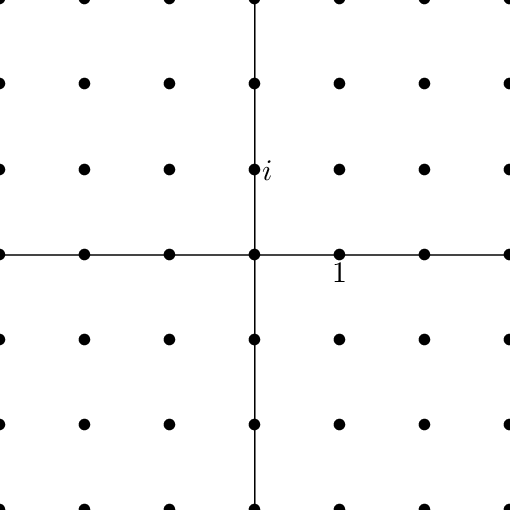
\includegraphics[scale=0.29]{Image/lattice-Z[i].png}
    \caption{Lattice formed by $\mathbb{Z}[\mathrm{i}]$}
\end{figure}
Now we would like to generalize the preceding idea.
\begin{definition}
Let $V$ be a $n$-dimensional $\mathbb{R}$-vector space. A \textit{lattice} in $V$ is a subgroup of the form $\Gamma=\mathbb{Z}v_1+\cdots+\mathbb{Z}v_m$, with linearly independent vectors $v_1,\cdots,v_m$ of $V$. The $m$-tuple $(v_1,\cdots,v_m)$ is called a \textit{basis} and the set 
$$
\Phi =\left\{ x_1v_1+\cdots +x_mv_m:x_i\in \mathbb{R} ,0\le x_i<1 \right\} 
$$
is a \textit{fundamental mesh} of the lattice. The lattice is said to be \textit{complete} or a \textit{$\mathbb{Z}$-structure} of $V$ if $m=n$.
\end{definition}
We make some comments on the preceding definition. First of all we have every lattice is finitely generated. However the converse is not generally true, for instance consider $\mathbb{Z}+\mathbb{Z}\sqrt{2}$. Secondly, note that every lattice is a \textit{discrete subgroup} of $V$, i.e. every point $\gamma\in\Gamma$ is an isolated point in the sense that there exists a neighborhood which contains no other points of $\Gamma$. In fact, if $\gamma=a_1v_1+\cdots+a_mv_m\in\Gamma$, then extending $v_1,\cdots,v_m$ into a basis of $V$ and consider the set 
$$
\left\{ x_1v_1+\cdots +x_nv_n:x_i\in \mathbb{R} ,\left| a_i-x_i \right|<1,i=1,2,\cdots ,m \right\} .
$$
We will further discover that this property is indeed characteristic.
\begin{proposition}
A subgroup $\Gamma\subset V$ is a lattice if and only if it is discrete.
\end{proposition}
\begin{proof}
We have shown that a lattice is a discrete subgroup, now we prove the converse. Suppose $D$ is a discrete subgroup of $V$. Let $\alpha_1,\cdots,\alpha_m$ be a basis of the vector space $V_0$ spanned by $D$, and let $P$ be the polyhedron with vertices $\alpha_1,\cdots,\alpha_m$, then the group $D\cap P$ is finite. Now suppose $x\in D$, we claim that $x$ lies in the free generated abelian group $(P\cap D)\{\alpha_1,\cdots,\alpha_m\}$. To see this, suppose $x=\sum_{i=1}^m\lambda_i\alpha_i$, where $\lambda_i\in\mathbb{R}$, and define 
$$
x_j=jx-\sum_{i=1}^m{\lfloor j\lambda _i \rfloor \alpha _i}=\sum_{i=1}^m{\left\{ j\lambda _i \right\} \alpha _i}\in D\cap P.
$$
Then we have 
$$
x_1+\sum_{i=1}^m{\lfloor \lambda _i \rfloor \alpha _i}=x-\sum_{i=1}^m{\lfloor \lambda _i \rfloor \alpha _i}+\sum_{i=1}^m{\lfloor \lambda _i \rfloor \alpha _i}=x,
$$
hence $D$ is a finitely generated abelian group. On the other hand, since $P\cap D$ is finite and $\mathbb{Z}$ is infinite, there exists $j$ and $k$ such that $x_j=x_k$ with $j\ne k$, hence 
$$
0=x_j-x_k=\sum_{i=1}^m{\lfloor k\lambda _i \rfloor \alpha _i}-\sum_{i=1}^m{\lfloor j\lambda _i \rfloor \alpha _i}=\sum_{i=1}^m{\left( \lfloor k\lambda _i \rfloor -\lfloor j\lambda _i \rfloor \right) \alpha _i},
$$
which implies $\lfloor k\lambda _i \rfloor -\lfloor j\lambda _i \rfloor =\left( k-j \right) \lambda _i\in \mathbb{Z} $, and hence $\lambda_i\in\mathbb{Q}$, therefore there exists some $d\in\mathbb{Z}$ such that $dD\cong \mathbb{Z} \alpha _1\oplus \cdots \oplus \mathbb{Z} \alpha _m$. Now note that $r\le \mathrm{rank}\left( D \right) =\mathrm{rank}\left( dD \right) \le r$, we have $\mathrm{rank}(D)=r$ and hence by the main theorem on finitely generated abelian groups, there exists $\{f_1,\cdots,f_m\}$ such that $D=\mathbb{Z} f_1/d\oplus \cdots \oplus \mathbb{Z} f_m/d$, which is a lattice.
\end{proof}
We now give some characterizations of a lattice to be complete.
\begin{proposition}
A lattice $\Gamma\subset\mathbb{R}^n$ is complete if and only if there exists a bounded subset $M\subset V$ such that the collection of all translates $M+\gamma$, $\gamma\in\Gamma$, covers the entire space $V$.
\end{proposition}
\begin{proof}
If $\Gamma=\mathbb{Z}v_1+\cdots\mathbb{Z}v_n$ is complete, then one may take $M$ to be the fundamental mesh $\Phi=\{x_1v_1+\cdots+x_nv_n:0\le x_i<1\}$.\par
Conversely, suppose $M$ is a bounded subset of $V$ whose translates $M+\gamma$ covers $V$. Let $V_0$ be the subspace spanned by $\Gamma$. We have to show that $V=V_0$. Let $v\in V$. Since $V=\bigcup_{\gamma\in\Gamma}(M+\gamma)$ we may write, for each $n\in\mathbb{N}$ we have 
$$
nv=a_n+\gamma _n,\hspace{0.5cm}\left( a_n\in M,\gamma _n\in \Gamma \subset V_0 \right) 
$$
since $M$ is bounded, $a_n/n$ converges to zero, and since $V_0$ is closed, 
$$
v=\lim_{n\rightarrow \infty} \frac{a_n}{n}+\lim_{n\rightarrow \infty} \frac{\gamma _n}{n}=\lim_{n\rightarrow \infty} \frac{\gamma _n}{n}\in V_0,
$$
which finished the proof.
\end{proof}
\begin{corollary}
A lattice $\Gamma\subset\mathbb{R}^n$ is complete if and only if the quotient $\mathbb{R}^n/\Gamma$ is compact.
\end{corollary}
\begin{proof}
Suppose first $\Gamma$ is complete, then the closure of the fundamental mash 
$$
\bar{\Phi}=\left\{ x_1v_1+\cdots +x_nv_n:0\le x_i\le 1 \right\} 
$$
is compact in $\mathbb{R}^n$. Note that the canonical map $\mathbb{R}^n\to\mathbb{R}/\Gamma$ is continuous, hence the image of $\bar{\Phi}$ under the canonical map is compact. However, the image of $\bar{\Phi}$ is $\mathbb{R}^n/\Gamma$, which finished the proof.\par
Conversely, suppose $\Gamma$ is a lattice of $\mathbb{R}^n$ such that $\mathbb{R}^n/\Gamma$ is compact. We show that $\Gamma$ is complete. Let $W$ be the subspace generated by the basis of $\Gamma$, then $\mathbb{R}^n/W$ must have dimension zero, or otherwise the quotient $\mathbb{R}^n/\Gamma$ is unbounded, and hence not compact, a contradiction! Therefore $W=\mathbb{R}^n$ and hence $\Gamma$ is complete. 
\end{proof}
We now introduce the concept of volumes of lattices. Let $V$ be a Euclidean space, i.e. an $\mathbb{R}$-vector space of finite dimension $n$ equipped with a symmetric, positive definite bilinear form $\left<\cdot,\cdot\right>:V\times V\to\mathbb{R}$. Then we have on $V$ a notion of volume, or more precisely, a Haar measure. The cube spanned by an orthonormal basis $e_1,\cdots,e_n$ has volume $1$, and more generally, the parallelepiped spanned by $n$ linearly independent vectors $v_1,\cdots,v_n$, the fundamental mash 
$$
\Phi =\left\{ x_1v_1+\cdots +x_nv_n:x_i\in \mathbb{R} ,0\le i<1 \right\} 
$$
has volume $\mathrm{vol}(\Phi)=|\det A|$, where $A=(a_{ik})$ is the matrix of the base change from $e_1,\cdots,e_n$ to $v_1,\cdots,v_n$, so that $v_i=\sum_ka_{ik}e_k$. Since 
$$
\left( \left< v_i,v_j \right> \right) =\left( \left< \sum_k{a_{ik}e_k},\sum_l{a_{jl}e_l} \right> \right) =\left( \sum_k{\sum_l{a_{ik}a_{jl}\left< e_k,e_l \right>}} \right) =\left( \sum_k{a_{ik}a_{jk}} \right) =AA^{\mathrm{T}},
$$
which also gives the invariant notation $\mathrm{vol}(\Phi)=|\det(\left<v_i,v_j\right>)|^{1/2}$.\par
Let $\Gamma$ be the lattice spanned by $v_1,\cdots,v_n$. Then $\Phi$ is a fundamental mesh of $\Gamma$, and we write for short $\mathrm{vol}(\Gamma)=\mathrm{vol}(\Phi)$. This does not depend on the choice of a basis $v_1,\cdots,v_n$ of the lattice because the transition matrix passing to a different basis, as well as its inverse, has integer coefficients, and therefore has determinant $\pm 1$ so that the set $\Phi$ is transformed into a set of the same volume.\par
Before introducing the following theorem, we give some terminologies. A subset $X$ of $V$ is called \textit{centrally symmetric}, if, given any point $x\in X$, the point $-x\in X$. $X$ is said to be \textit{convex} if, given any two points $x,y\in X$ we have $tx+(1-t)y\in X$ for all $t\in (0,1)$.
\begin{theorem}
Let $\Gamma$ be a complete lattice in the Euclidean vector space $V$ and $X$ a centrally symmetric, convex subset of $V$. Suppose that $\mathrm{vol}(X)>2^n\mathrm{vol}(\Gamma)$, then $X$ contains at least one nonzero lattice point $\gamma\in\Gamma$.
\end{theorem}
\begin{proof}
It suffices to show that there exist two distinct lattice points $\gamma_1,\gamma_2\in\Gamma$ such that 
$$
\left( \frac{1}{2}X+\gamma _1 \right) \cap \left( \frac{1}{2}X+\gamma _2 \right) \ne \emptyset .
$$
Now suppose the sets $1/2X+\gamma$, $\gamma\in\Gamma$ were pairwise disjoint, then the same would be true of their intersections $\Phi\cap(1/2X+\gamma)$ with a fundamental mash $\Phi$ of $\Gamma$, i.e. 
$$
\mathrm{vol}\left( \Phi \right) \ge \sum_{\gamma \in \Gamma}{\mathrm{vol}\left( \Phi \cap \left( \frac{1}{2}X+\gamma \right) \right)}=\mathrm{vol}\left( \frac{1}{2}X \right) =\frac{1}{2^n}\mathrm{vol}\left( X \right) ,
$$
a contradiction!
\end{proof}
Minkowski's theorem will be applied to various sets in the next section. To avoid distraction then, we do some volume calculations here.
\begin{proposition}
Let $n=r+2s$ for nonnegative integers $r$ and $s$ and let points in the $n$-dimensional $\mathbb{R}$-vector space $V$ be represented by the usual $n$ tuples.
\begin{enumerate}
    \item Let $c_1,\cdots,c_{r+s}$ be positive integers and 
    $$
    X=\left\{ \left( x_1,\cdots ,x_r,y_1,z_1,\cdots ,y_s,z_s \right) :\left| x_i \right|<c_i,y_{j}^{2}+z_{j}^{2}<c_{r+j} \right\} ,
    $$
    where $1\le i\le r$ and $1\le j\le s$. Then $\mathrm{vol}(X)=2^r\pi^s\prod_{i=1}^{r+s}c_i$.
    \item For any positive integer $t$ let 
    $$
    X_t=\left\{ \left( x_1,\cdots ,x_r,y_1,z_1,\cdots ,y_s,z_s \right) :\sum_{i=1}^r{\left| x_i \right|}+2\sum_{j=1}^s{\sqrt{y_{j}^{2}+z_{j}^{2}}}<t \right\} .
    $$
    Then 
    $$
    \mathrm{vol}\left( X_t \right) =\frac{2^{r-s}\pi ^st^n}{n!}.
    $$
\end{enumerate}
\end{proposition}
\begin{proof}
The first statement is trivial, for $X$ is a product of $r$ intervals with length $2c_i$ and $s$ spheres with radii $\sqrt{c_{r+j}}$. Therefore 
$$
\mathrm{vol}\left( X \right) =\prod_{i=1}^r{\left( 2c_i \right)}\cdot \prod_{j=1}^s{\pi \left( \sqrt{c_{r+j}} \right) ^2}=2^r\pi ^s\prod_{k=1}^{r+s}{c_k}.
$$
Now for the second statement, we begin by writing $v_{r,s}(t)=\mathrm{vol}(X_t)$. Take the substitution 
$$
\begin{cases}
	2y_j=\rho _j\cos \phi _j,\\
	2z_j=\rho _j\sin \phi _j,\\
	4\mathrm{d}y_j\mathrm{d}z_j=\rho _j\mathrm{d}\rho _j\mathrm{d}\phi _j,\\
\end{cases}
$$
and taking only the region having $x_i\ge 0$ for $1\le i\le r$ so that 
$$
\begin{aligned}
v_{r,s}\left( t \right) &=\int_{X_t}{\mathrm{d}x_1\cdots \mathrm{d}x_r\mathrm{d}y_1\cdots \mathrm{d}y_s\mathrm{d}z_1\cdots \mathrm{d}z_s}
\\
&=2^r2^{-2s}\int_{X_{t}^{\prime}}{\rho _1\cdots \rho _s\mathrm{d}x_1\cdots \mathrm{d}x_r\mathrm{d}\rho _1\cdots \mathrm{d}\rho _s\mathrm{d}\phi _1\cdots \mathrm{d}\phi _s}
\\
&=2^r2^{-2s}\left( 2\pi \right) ^s\int_{Y_t}{\rho _1\cdots \rho _s\mathrm{d}x_1\cdots \mathrm{d}x_r\mathrm{d}\rho _1\cdots \mathrm{d}\rho _s},
\end{aligned}
$$
where 
$$
Y_t=\left\{ \left( x_1,\cdots ,x_r,\rho _1,\cdots ,\rho _s \right) :x_i\ge 0,\rho _j\ge 0,\sum_{i=1}^r{x_i}+\sum_{j=1}^s{\rho _j}<t \right\} .
$$
Let 
$$
w_{r,s}\left( t \right) =\int_{Y_t}{\rho _1\cdots \rho _s\mathrm{d}x_1\cdots \mathrm{d}x_r\mathrm{d}\rho _1\cdots \mathrm{d}\rho _s},
$$
then 
$$
w_{r,s}\left( t \right) =t^{r+2s}w_{r,s}\left( 1 \right) =t^nw_{r,s}\left( 1 \right) .
$$
This homogeneity condition allows the integral $w_{r,s}(1)$ to be evaluated. Note that 
$$
w_{r,s}\left( 1 \right) =\int_0^1{w_{r-1,s}\left( 1-x_1 \right) \mathrm{d}x_1}=w_{r-1,s}\left( 1 \right) \int_0^1{x_{1}^{r-1+2s}\mathrm{d}x_1}=\frac{w_{r-1,s}\left( 1 \right)}{r+2s},
$$
we have 
$$
w_{r,s}\left( 1 \right) =\frac{1}{r+2s}w_{r-1,s}\left( 1 \right) =\cdots =\frac{\left( 2s \right) !}{\left( r+2s \right) !}w_{0,s}\left( 1 \right) .
$$
Now it suffices to evaluate $w_{0,s}(1)$. Note that 
$$
w_{0,s}\left( 1 \right) =\int_0^1{\rho _sw_{0,s-1}\left( 1-\rho _s \right) \mathrm{d}\rho _s}=w_{0,s-1}\left( 1 \right) \int_0^1{\rho _s\left( 1-\rho _s \right) ^{2s-2}\mathrm{d}\rho _s}=\frac{w_{0,s-1}\left( 1 \right)}{\left( 2s \right) \left( 2s-1 \right)},
$$
we have 
$$
w_{0,s}\left( 1 \right) =\frac{w_{0,s-1}\left( 1 \right)}{\left( 2s \right) \left( 2s-1 \right)}=\cdots =\frac{1}{\left( 2s \right) !}
$$
and hence 
$$
w_{r,s}\left( 1 \right) =\frac{\left( 2s \right) !}{\left( r+2s \right) !}w_{0,s}\left( 1 \right) =\frac{1}{\left( r+2s \right) !},
$$
which finished the proof.
\end{proof}
\subsection{The Class Number and the Unit Theorem}
In this section $K$ denotes a number field and $\mathcal{O}_K$ denote the algebraic numbers over $K$. The class group $\mathbf{C}(\mathcal{O}_K)$ was defined as the quotient of ideal group over the group of principle ideals. In this section we shall show that $\mathbf{C}(\mathcal{O}_K)$ is finite. We also determine the structure of the group of units of $\mathcal{O}_K$, which may seems quite different, but the methods used to prove them are very similar.\par
We shall first make some assumptions on the notations. Let $E$ be a normal extension field of $\mathbb{Q}$ containing $K$, $G=\mathrm{Gal}(E/\mathbb{Q})$ the Galois group of $E$ over $\mathbb{Q}$ and $H=\mathrm{Gal}(E/K)$ the subgroup of $G$. We regard $E$ as a subfield of $\mathbb{C}$ and hence each element of $G$ is an embedding of $E$ to $\mathbb{C}$.\par
Let $\sigma_1,\cdots,\sigma_n$ represent the distinct cosets $\sigma H$ in $G$. Then $n=[K:\mathbb{Q}]$ and $\sigma_i$'s are distinct embeddings of $K$ into $\mathbb{C}$. We may select the numbering so that $\sigma_1,\cdots,\sigma_r$ maps $K$ into $\mathbb{R}$, and the rest appear in pairs, say $\sigma_{r+1},\bar{\sigma}_{r+1},\cdots,\sigma_{r+s},\bar{\sigma}_{r+s}$, which maps $K$ into $\mathbb{C}$. Here $\bar{\sigma}_j(x)$ is defined to be the conjugate of $\sigma_j(x)$.\par
Now consider the function 
$$
v^*:K\rightarrow \mathbb{R} ^r\rightarrow \mathbb{C} ^s,\hspace{0.5cm}x\mapsto \left( \sigma _1\left( x \right) ,\cdots ,\sigma _r\left( x \right) ,\sigma _{r+1}\left( x \right) \cdots ,\sigma _{r+s}\left( x \right) \right) .
$$
It is clear that $v^*$ is an additive map, for $v^*(x+y)=v^*(x)+v^*(y)$. Since $\mathbb{C}$ has a natural structure as a two dimensional $\mathbb{R}$ space, we may see $\mathbb{R}^r\times\mathbb{C}^s$ as $\mathbb{R}^{r+2s}$ and define $v:K\to\mathbb{R}^{r+2s}$ by
$$
x\mapsto \left( \sigma _1\left( x \right) ,\cdots ,\sigma _r\left( x \right) ,\mathrm{Re}\left( \sigma _{r+1}\left( x \right) \right) ,\mathrm{Im}\left( \sigma _{r+1}\left( x \right) \right) ,\cdots ,\mathrm{Re}\left( \sigma _{r+s}\left( x \right) \right) ,\mathrm{Im}\left( \sigma _{r+s}\left( x \right) \right) \right) 
$$
Therefore $v(x)$ is a vector with $r+2s=n$ real coordinates.\par
We first make a calculation which will be used in the sequence.
\begin{lemma}\em\label{Computa1}
Let $a_1,\cdots,a_n$ be a basis for $K$ over $\mathbb{Q}$ and let $M=[v(a_i)]$ be the $n\times n$ real matrix having row $i$ equal to the vector $v(a_i)$ and let $D$ be the $n\times n$ matrix with row $i$ equal to 
$$
\left( \sigma _1\left( x \right) ,\cdots ,\sigma _r\left( x \right) ,\sigma _{r+1}\left( x \right) ,\bar{\sigma}_{r+1}\left( x \right) ,\cdots ,\sigma _{r+s}\left( x \right) ,\bar{\sigma}_{r+s}\left( x \right) \right) .
$$
Then 
$$
\det \left( M \right) =\left( -2\mathrm{i} \right) ^{-s}\det \left( D \right) ,
$$
where $\mathrm{i}=\sqrt{-1}$.
\end{lemma}
\begin{proof}
Note that 
$$
\begin{aligned}
D&=\left[ \begin{matrix}
	&		&		&		\vdots&		&		&		&		\\
	\sigma _1\left( x \right)&		\cdots&		\sigma _r\left( x \right)&		\sigma _{r+1}\left( x \right)&		\bar{\sigma}_{r+1}\left( x \right)&		\cdots&		\sigma _{r+s}\left( x \right)&		\bar{\sigma}_{r+s}\left( x \right)\\
	&		&		&		\vdots&		&		&		&		\\
\end{matrix} \right] 
\\
&\rightarrow \left[ \begin{matrix}
	&		&		&		\vdots&		&		&		&		\\
	\sigma _1\left( x \right)&		\cdots&		\sigma _r\left( x \right)&		2\mathrm{Re}\left( \sigma _{r+1}\left( x \right) \right)&		\bar{\sigma}_{r+1}\left( x \right)&		\cdots&		2\mathrm{Re}\left( \sigma _{r+s}\left( x \right) \right)&		\bar{\sigma}_{r+s}\left( x \right)\\
	&		&		&		\vdots&		&		&		&		\\
\end{matrix} \right] 
\\
&\rightarrow \left[ \begin{matrix}
	&		&		&		\vdots&		&		&		&		\\
	\sigma _1\left( x \right)&		\cdots&		\sigma _r\left( x \right)&		2\mathrm{Re}\left( \sigma _{r+1}\left( x \right) \right)&		\mathrm{i}\cdot \mathrm{Im}\left( \sigma _{r+1}\left( x \right) \right)&		\cdots&		2\mathrm{Re}\left( \sigma _{r+s}\left( x \right) \right)&		\mathrm{i}\cdot \mathrm{Im}\left( \sigma _{r+s}\left( x \right) \right)\\
	&		&		&		\vdots&		&		&		&		\\
\end{matrix} \right] ,
\end{aligned}
$$
therefore $\det \left( D \right) =2^s\cdot \mathrm{i}^s\cdot \det \left( M \right) $, which finished the proof.
\end{proof}
\begin{definition}
Let $\mathfrak{A}$ be a fractional ideal of $\mathcal{O}_K$ in the number field $K$. The \textit{discriminant} $\Delta(\mathfrak{A}/\mathbb{Z})$ of $\mathfrak{A}$ is the ideal $\mathbb{Z}$ generated by the discriminants $\Delta(a_1,\cdots,a_n)$ where $a_1,\cdots,a_n$ runs through all the bases of $K$ over $\mathbb{Q}$ contained in $\mathfrak{A}$.
\end{definition}
We may use the preceding lemma to give an expression of $\Delta(\mathfrak{A}/\mathbb{Z})$.
\begin{proposition}\label{DeltaA/Zchara}
For a fractional ideal $\mathfrak{A}$ of $\mathcal{O}_K$, let $a_1,\cdots,a_n$ be a free $\mathbb{Z}$-basis of $\mathfrak{A}$. The discriminant of $\mathfrak{A}$ and the real matrix $M=[v(a_i)]$ are related by the equation 
$$
\Delta \left( \mathfrak{A} /\mathbb{Z} \right) =\left( -4 \right) ^s\det \left( M \right) ^2.
$$
\end{proposition}
\begin{proof}
Let $D$ be the matrix defined in Lemma \ref{Computa1}, Then the $i,j$-entry of $DD^\mathrm{T}$ is 
$$
\sum_{p=1}^r{\sigma _p\left( a_i \right) \sigma _p\left( a_j \right)}+\sum_{q=1}^s{\sigma _{r+q}\left( a_i \right) \sigma _{r+q}\left( a_j \right)}+\sum_{q=1}^s{\bar{\sigma}_{r+q}\left( a_i \right) \bar{\sigma}_{r+q}\left( a_j \right)}=\mathrm{Tr}_{K/\mathbb{Q}}\left( a_ia_j \right) .
$$
Therefore 
$$
\Delta \left( a_1,\cdots ,a_n \right) =\det \left( D \right) ^2=\left( -4 \right) ^s\det \left( M \right) ^2,
$$
which finished the proof.
\end{proof}
A trivial corollary of Proposition \ref{DeltaA/Zchara} is that $\Delta(a_1,\cdots,a_n)$ is positive if and only if the number $s$ of pairs of non-real embeddings of $K$ into $\mathbb{C}$ is even.\par
We relate the discriminant of $\mathfrak{A}$ to the discriminant of $\mathcal{O}_K$ in the following.
\begin{proposition}\label{N(A)^2Delta(R/Z)}
The discriminant of a fractional ideal $\mathfrak{A}$ and the discriminant of $\mathcal{O}_K$ satisfies the equation 
$$
\Delta \left( \mathfrak{A} /\mathbb{Z} \right) =\mathcal{N} \left( \mathfrak{A} \right) ^2\Delta \left( \mathcal{O} _K/\mathbb{Z} \right) ,
$$
where $\mathcal{N}(\mathfrak{A})$ denote the number of elements in $\mathcal{O}_K/\mathfrak{A}$.
\end{proposition}
\begin{proof}
It suffices to show the equality holds at every localization of the maximal ideal of $\mathbb{Z}$. Let $p$ be a prime integer and $S=\mathbb{Z}-(p)$. Note that $(\mathcal{O}_K)_S$ is a PID with only a finite number of maximal ideals, therefore we may write $\mathfrak{A}_S=a(\mathcal{O}_K)_S$ for some $a\in(\mathcal{O}_K)_S$. Let $x_1,\cdots,x_n$ be a basis of $\mathcal{O}_K$ over $\mathbb{Z}$, then it is also a basis of $(\mathcal{O}_K)_S$ over $\mathbb{Z}_{(p)}$. Therefore $ax_1,\cdots,ax_n$ is a basis of $\mathcal{O}_K$ of $\mathfrak{A}_S$. Let $\rho_a$ be the matrix of the regular representation $r_a:y\mapsto ya$ with respect to the basis $x_1,\cdots,x_n$. Then we have 
$$
\left[ \mathrm{Tr}_{K/\mathbb{Q}}\left( ax_iax_j \right) \right] =\rho _a\left[ \mathrm{Tr}_{K/\mathbb{Q}}\left( x_ix_j \right) \right] \rho _{a}^{\mathrm{T}}.
$$
But now $\mathrm{N}_{K/\mathbb{Q}}(a)=\det(\rho_a)$, hence 
$$
\det \left( ax_1,\cdots ,ax_n \right) =\det \left( \rho _a\left[ \mathrm{Tr}_{K/\mathbb{Q}}\left( x_ix_j \right) \right] \rho _{a}^{\mathrm{T}} \right) =\mathrm{N}_{K/\mathbb{Q}}\left( a \right) ^2\Delta \left( x_1,\cdots ,x_n \right) .
$$
Use the equation 
$$
\mathrm{N}_{K/\mathbb{Q}}\left( \mathfrak{A} _S \right) =\mathrm{N}_{K/\mathbb{Q}}\left( a \right) \mathbb{Z} _{\left( p \right)}=\mathcal{N} \left( \mathfrak{A} \right) \mathbb{Z} _{\left( p \right)}
$$
to conclude that 
$$
\Delta \left( \mathfrak{A} /\mathcal{O} _K \right) _S=\Delta \left( \mathfrak{A} _S/\left( \mathcal{O} _K \right) _S \right) =\mathcal{N} \left( \mathfrak{A} _S \right) ^2\Delta \left( \left( \mathcal{O} _K \right) _S/\mathbb{Z} _{\left( p \right)} \right) =\Delta \left( \mathcal{O} _K/\mathbb{Z} \right) _S,
$$
which finished the proof.
\end{proof}
Now we apply these computations to describe some lattices.
\begin{theorem}
Let $\mathfrak{A}$ be a nonzero ideal in the ring $\mathcal{O}_K$ of algebraic integers in an algebraic number field $K$. Let $v:K\to\mathbb{R}^n$ be defined in the preceding contents. Then $v(\mathfrak{A})$ is a full lattice in $\mathbb{R}^n$ with volume $2^{-s}\mathcal{N}(\mathfrak{A})|\Delta(\mathcal{O}_K/\mathbb{Z})|^{1/2}$.
\end{theorem}
\begin{proof}
Let $a_1,\cdots,a_n$ be a $\mathbb{Z}$-basis of $\mathfrak{A}$. Then $v(a_1),\cdots,v(a_n)$ is a $\mathbb{Z}$-basis for $v(\mathfrak{A})$. To show that $v(\mathfrak{A})$ is a lattice, it suffices to show that the vectors $v(a_1),\cdots,v(a_n)$ are linearly independent over $\mathbb{R}$. If $M$ is the matrix with $i$-th row equal to the vector $v(a_i)$, then $\det M\ne 0$ and in fact, the volume of the lattice equals to $\det M=2^{-s}|\Delta(\mathcal{O}_K/\mathbb{Z})|^{1/2}$. Now by Proposition \ref{N(A)^2Delta(R/Z)} we finished the proof.
\end{proof}
Now we have several general facts available about lattices and discriminants, we make the first important step in the proof that the ring of algebraic integers in $K$ has only a finite number of ideal classes.
\begin{theorem}\label{MinBoundLem}
Let $\mathfrak{A}$ be a nonzero ideal of $\mathcal{O}_K$. Then there exists an element $a\ne 0$ in $\mathfrak{A}$ such that 
$$
\left| \mathrm{N}_{K/\mathbb{Q}}\left( a \right) \right|\le \frac{n!}{n^n}\left( \frac{4}{\pi} \right) ^s\mathcal{N} \left( \mathfrak{A} \right) \left| \Delta \left( \mathcal{O} _K/\mathbb{Z} \right) \right|^{\frac{1}{2}}.
$$
\end{theorem}
\begin{proof}
The main tool in the proof of the theorem is Minkowski's Theorem, which ensures the existence of a lattice point in a suitable set. Let 
$$
X_t=\left\{ \left( x_1,\cdots ,x_r,y_1,z_1,\cdots ,y_s,z_s \right) :\sum_{i=1}^r{\left| x_r \right|}+2\sum_{j=1}^s{\sqrt{y_{j}^{2}+z_{j}^{2}}}<t \right\} .
$$
This is a convex central symmetric subset of $\mathbb{R}^n$ with volume $\mathrm{vol}\left( X_t \right) =2^{r-s}\pi ^st^n/n!$. Now if $\mathrm{vol}(X_t)>2^n\mathrm{vol}(\mathfrak{A})$ then $X_t$ contains a nonzero point of $v(\mathfrak{A})$. This inequality holds if 
$$
2^{r-s}\pi ^s\frac{t^n}{n!}>2^{n-s}\mathcal{N} \left( \mathfrak{A} \right) \left| \Delta \left( \mathcal{O} _K/\mathbb{Z} \right) \right|^{\frac{1}{2}},
$$
therefore take 
$$
t^n=\varepsilon +n!\left( \frac{2^{n-r}}{\pi ^s} \right) \mathcal{N} \left( \mathfrak{A} \right) \left| \Delta \left( \mathcal{O} _K/\mathbb{Z} \right) \right|^{\frac{1}{2}},
$$
we have a point in $X_t\cap v(\mathfrak{A})$ as $\varepsilon\to 0$. Since a lattice is a discrete subgroup of $\mathbb{R}^n$, we have the convergent point is nonzero even if $\varepsilon=0$. Suppose the convergent point is 
$$
\begin{aligned}
v\left( a \right) &=\left( \sigma _1\left( a \right) ,\cdots ,\sigma _r\left( a \right) ,\mathrm{Re}\left( \sigma _{r+1}\left( a \right) \right) ,\mathrm{Im}\left( \sigma _{r+1}\left( a \right) \right) ,\cdots ,\mathrm{Re}\left( \sigma _{r+s}\left( a \right) \right) ,\mathrm{Im}\left( \sigma _{r+s}\left( a \right) \right) \right) 
\\
&=\left( x_1,\cdots ,x_r,y_1,z_1,\cdots ,y_s,z_s \right) .
\end{aligned}
$$
Now 
$$
\left| \mathrm{N}_{K/\mathbb{Q}}\left( a \right) \right|=\prod_{i=1}^r{\left| \sigma _i\left( a \right) \right|}\prod_{j=1}^s{\left| \sigma _{r+j}\left( a \right) \right|^2}=\prod_{i=1}^r{\left| x_i \right|}\prod_{j=1}^s{\left( y_{j}^{2}+z_{j}^{2} \right)},
$$
therefore by the Arithmetic-Geometric Inequality, we have 
$$
\left| \mathrm{N}_{K/\mathbb{Q}}\left( a \right) \right|^{\frac{1}{n}}\le \frac{1}{n}\left( \sum_{i=1}^r{\left| x_i \right|}+2\sum_{i=1}^s{\sqrt{y_{j}^{2}+z_{j}^{2}}} \right) <\frac{t}{n},
$$
hence 
$$
\left| \mathrm{N}_{K/\mathbb{Q}}\left( a \right) \right|\le \frac{t^n}{n^n}=\frac{n!}{n^n}\left( \frac{4}{\pi} \right) ^s\mathcal{N} \left( \mathfrak{A} \right) \left| \Delta \left( \mathcal{O} _K/\mathbb{Z} \right) \right|^{\frac{1}{2}}.
$$
This finished the proof.
\end{proof}
Recall that the class group $\mathbf{C}(\mathcal{O}_K)$ is the quotient of the group of fractional ideals of $\mathcal{O}_K$ by the subgroup of principal ideals; alternatively this is the set of equivalence classes of nonzero fractional ideals of $\mathcal{O}_K$ where two ideals $\mathfrak{A}$ and $\mathfrak{B}$ are equivalent if and only if $\mathfrak{A}=\mathfrak{B}c$ for some $c\in K$. The equivalent class of $\mathfrak{A}$ is denoted by $[\mathfrak{A}]$.
\begin{theorem}{(\textit{The Minkowski's Bound})}\label{MinBound}
For any nonzero fractional ideal $\mathfrak{B}$ of $\mathcal{O}_K$ there is an $\mathfrak{A}\in[\mathfrak{B}]$ such that $\mathfrak{A}\subset\mathcal{O}_K$ and 
$$
\mathcal{N} \left( \mathfrak{A} \right) \le \frac{n!}{n^n}\left( \frac{4}{\pi} \right) ^s\left| \Delta \left( \mathcal{O} _K/\mathbb{Z} \right) \right|^{\frac{1}{2}}.
$$
\end{theorem}
\begin{proof}
Take any $b\in\mathfrak{B}$, then $b\mathfrak{B}^{-1}$ is an ideal of $\mathcal{O}_K$ lying in the equivalence class $[\mathfrak{B}^{-1}]$. Therefore by Theorem \ref{MinBoundLem} there exists some $a\in b\mathfrak{B}^{-1}$ such that 
$$
\left| \mathrm{N}_{K/\mathbb{Q}}\left( a \right) \right|\mathcal{N} \left( \mathfrak{B} \right) ^{-1}\le \frac{n!}{n^n}\left( \frac{4}{\pi} \right) ^s\left| \Delta \left( \mathcal{O} _K/\mathbb{Z} \right) \right|^{\frac{1}{2}}.
$$
Set $\mathfrak{A}=a\mathfrak{B}^{-1}$. Then since $a\in\mathfrak{B}_1$ we have $\mathfrak{A}\subset\mathcal{O}_K$, and 
$$
\mathcal{N} \left( \mathfrak{A} \right) =\mathcal{N} \left( a\mathfrak{B} ^{-1} \right) =\left| \mathrm{N}_{K/\mathbb{Q}}\left( a \right) \right|\mathcal{N} \left( \mathfrak{B} _1 \right) ^{-1}\le \frac{n!}{n^n}\left( \frac{4}{\pi} \right) ^s\left| \Delta \left( \mathcal{O} _K/\mathbb{Z} \right) \right|^{\frac{1}{2}},
$$
which is 
$$
\mathcal{N} \left( \mathfrak{A} \right) \le \frac{n!}{n^n}\left( \frac{4}{\pi} \right) ^s\left| \Delta \left( \mathcal{O} _K/\mathbb{Z} \right) \right|^{\frac{1}{2}}.
$$
This finished the proof.
\end{proof}
We now come to the theorem of the finiteness of $\mathbf{C}(\mathcal{O}_K)$.
\begin{theorem}
The ideal class group of the ring of algebraic integers in an algebraic number field is finite.
\end{theorem}
\begin{proof}
Recall that $\mathcal{N}(\mathfrak{A})=|\mathcal{O}_K/\mathfrak{A}|$. Since $\mathcal{N}(\mathfrak{A})$ is bounded, it suffices to show that there are only a finite number of integral ideals with norm below the fixed bound.\par
Let $\mathfrak{A}=\mathfrak{P}_1^{a_1}\cdots\mathfrak{P}_t^{a_t}$ be a nonzero ideal of $\mathcal{O}_K$, $\mathfrak{P}_i$ distinct primes and the $a_i$ positive integers. Let $p_i\mathbb{Z}=\mathfrak{P}_i\cap\mathbb{Z}$, where $p_i$ is a positive prime integer. Suppose 
$$
\mathcal{N} \left( \mathfrak{A} \right) =\prod_{i=1}^t{p_{i}^{f_ia_i}}\le \frac{n!}{n^n}\left( \frac{4}{\pi} \right) ^s\left| \Delta \left( \mathcal{O} _K/\mathbb{Z} \right) \right|^{\frac{1}{2}}.
$$
Then since each $p_i^{a_if_i}\le M$, where $M$ denote the right-hand-side constant, we know that there are only a finite number of possible $\mathfrak{P}_i$ and $a_i$. Therefore every ideal class is represented by one of finite number of ideals, hence $\mathbf{C}(\mathcal{O}_K)$ is finite.
\end{proof}
It is usually very difficult to calculate the class number of a field. However, for certain fields, the class number is relatively easy to calculate. We give an example.
\begin{example}\em
We return to the field $K=\mathbb{Q}(\theta)$ where $\theta^3=2$. The polynomial $X^3-2$ has one real root and two complex roots, therefore $r=s=1$ and $n=3$. The discriminant $\Delta=-2^2\cdot 3^2$ as calculated before, therefore 
$$
\mathcal{N} \left( \mathfrak{A} \right) \le \frac{3!}{3^3}\cdot \frac{4}{\pi}\cdot \sqrt{2^2\cdot 3^2}<2.94,
$$
therefore it suffices to determine the ideal $2\mathcal{O}_K=(\theta\mathcal{O}_K)^3$, where $\theta\mathcal{O}_K$ is of norm $2$. Therefore every ideal class contains a principal ideal, and hence the class number of $K$ is $1$ and every ideal is principal.
\end{example}
We can obtain information about the size of the discriminant from Theorem \ref{MinBound}. Every ideal of $\mathcal{O}_K$ has norm at least one. It follows that 
$$
\left| \Delta \left( \mathcal{O} _K/\mathbb{Z} \right) \right|^{\frac{1}{2}}\ge \frac{n^n}{n!}\left( \frac{\pi}{4} \right) ^s\ge \frac{n^n}{n!}\left( \frac{\pi}{4} \right) ^{\frac{n}{2}}.
$$
Let $a_n$ denote the rightmost expression. We compute 
$$
\frac{a_{n+1}}{a_n}=\left( \frac{\pi}{4} \right) ^{\frac{1}{2}}\left( 1+\frac{1}{n} \right) ^n>1,\hspace{0.5cm}\left( n>1 \right) 
$$
hence $a_{n+1}>a_n$. We have $a_2>1$ and hence $|\Delta|>1$ if $n\ge 2$. We therefore obtain the following theorem.
\begin{theorem}(\textit{Minkowski})
Let $\mathcal{O}_K$ be the ring of algebraic integers in an algebraic number field $K\ne\mathbb{Q}$. Then $\Delta(\mathcal{O}_K/\mathbb{Z})\ne\mathbb{Z}$. In particular some prime of $\mathbb{Z}$ must ramify in $\mathcal{O}_K$.
\end{theorem}
Note that this theorem is sensitive to the requirement that the base field is the rational field. For extensions of other number fields, it may happen that no prime ramifies. This topic will be considered in detail when we discuss the Hilbert Class Field. Now let's take a look at an example.
\begin{example}\em\label{Magma1}
Let $K=\mathbb{Q}(\sqrt{-5})$ and $L=K(\sqrt{5})$. We will show that no prime in the ring of algebraic integers of $K$ is ramified in $L$. By a computation via Magma (see appendix \ref{MagmaCode1} for further information) we have $\Delta(\mathcal{O}_L/\mathcal{O}_K)$ is a principal ideal, hence no prime in the ring of algebraic integers of $K$ is ramified in $L$.
\end{example}
Now we turn to the consideration of the group of units $U$ in the ring $\mathcal{O}_K$ of algebraic integers in an algebraic number field $K$. We continue with the notation introduced in the beginning of this section.\par
Define the function $l(a)$ for nonzero elements $a$ of $K$ by the rule 
$$
l\left( a \right) =\left( \log \left| \sigma _1\left( a \right) \right|,\cdots ,\log \left| \sigma _r\left( a \right) \right|,2\log \left| \sigma _{r+1}\left( a \right) \right|,\cdots ,2\log \left| \sigma _{r+s}\left( a \right) \right| \right) .
$$
For convenience we write the coordinates using 
$$
l_i\left( a \right) =\begin{cases}
	\log \left| \sigma _i\left( a \right) \right|,1\le i\le r,\\
	2\log \left| \sigma _i\left( a \right) \right|,r<i\le r+s.\\
\end{cases}
$$
It is obvious that $l(ab)=l(a)+l(b)$, therefore $l$ maps the multiplicative group of $K$ into the additive group of $r+s$-dimensional space $V_0=\mathbb{R}^{r+s}$. Our goal is to determine $l(U)$. We begin by showing it is  a lattice.
\begin{proposition}\label{lUlattice1}
The homomorphism $l$ maps the unit group $U$ of $\mathcal{O}_K$ onto a lattice in the $r+s-1$ dimensional subspace of $V_0=\mathbb{R}^{r+s}$ consisting of all vectors $(x_1,\cdots,x_{r+s})$ with $\sum x_i=0$.
\end{proposition}
\begin{proof}
For each $a\in U$ we have $\mathrm{N}_{K/\mathbb{Q}}(a)=\pm 1$. Therefore 
$$
\sum_{i=1}^{r+s}{l_i\left( a \right)}=\sum_{i=1}^r{\log \left| \sigma _i\left( a \right) \right|}+2\sum_{j=1}^s{\log \left| \sigma _{r+j}\left( a \right) \right|}=\log \left( \prod_{i=1}^n{\left| \sigma _i\left( a \right) \right|} \right) =\log \left| \mathrm{N}_{K/\mathbb{Q}}\left( a \right) \right|=0.
$$
This implies $l(U)$ lies in the hyperplane 
$$
V_0=\left\{ \left( x_1,\cdots ,x_{r+s} \right) :\sum_{i=1}^{r+s}{x_i=0} \right\} .
$$
Now we show $l(U)$ is a lattice. Suppose $m>0$, define 
$$
U_m=\left\{ a\in U:\left| l_i\left( a \right) \right|\le m,1\le i\le r+s \right\} ,
$$
then $l(U_m)$ is a cube of $l(U)$ with side-length $2m$. It suffices to show that $l(U_m)$ is finite. To see this, define 
$$
\delta _i=\begin{cases}
	1,1\le i\le r,\\
	2,r<i\le r+s,\\
\end{cases}
$$
we have 
$$
\left| \sigma _i\left( u \right) \right|\le \exp \left( \frac{m}{\delta _i} \right) .
$$
Now consider $v(U_m)$, which is the subgroup of the lattice $v(\mathcal{O}_K)$ and hence $v(U_m)$ is a finite set. But $v$ is a one-to-one mapping, therefore $U_m$ is finite and hence $l(U)$ is a lattice. This finished the proof.
\end{proof}
Our next goal is to improve this proposition to conclude that $l(U)$ is a full lattice in the $r+s-1$ dimensional subspace rather than just contained in it. We first work in the $n$-dimensional real vector space $W=\mathbb{R}^r\times\mathbb{C}^s$. Define a linear transformation $Y$ on $W$ by the rule 
$$
Y\left( x_1,\cdots ,x_{r+s} \right) =\left( x_1y_1,\cdots ,x_{r+s}y_{r+s} \right) ,
$$
where $y_i\in\mathbb{R}$ when $1\le i\le r$ and $y_j\in\mathbb{C}$ when $r<j\le r+s$. If we define 
$$
y_{j}^{*}=\left[ \begin{matrix}
	a&		b\\
	-b&		a\\
\end{matrix} \right] ,\hspace{0.5cm}\left( r+1\le j\le r+s,y_j=a+b\mathrm{i} \right) 
$$
then $Y$ has its matrix representation 
$$
M_Y=\mathrm{diag}\left( y_1,\cdots ,y_r,y_{r+1}^{*},\cdots ,y_{r+s}^{*} \right) 
$$
and hence 
$$
\det Y=y_1\cdots y_r\left| y_{r+1} \right|^2\cdots \left| y_{r+s} \right|^2.
$$
We impose $\det Y=1$ first. Therefore $Y$ preserves volume and hence 
$$
\mathrm{vol}\left( Yv^*\left( \mathcal{O} _K \right) \right) =\mathrm{vol}\left( v^*\left( \mathcal{O} _K \right) \right) =2^{-s}\left| \Delta \left( \mathcal{O} _K/\mathbb{Z} \right) \right|^{\frac{1}{2}}.
$$
Now consider a set $c_1,\cdots,c_{r+s}$ of positive constants and let 
$$
X=\left\{ \left( x_1,\cdots ,x_{r+s} \right) \in W:\left| x_i \right|\le c_i,\left| x_{r+j} \right|^2\le c_{r+j},1\le i\le r,1\le j\le s \right\} .
$$
The volume of $X$ was computed before with the result $\mathrm{vol}\left( X \right) =2^r\pi ^sc_1\cdots c_{r+s}$. Now we wish to apply Minkowski's theorem. We require 
$$
\mathrm{vol}\left( X \right) >2^n\mathrm{vol}\left( Yv^*\left( \mathcal{O} _K \right) \right) =2^{n-s}\left| \Delta \left( \mathcal{O} _K/\mathbb{Z} \right) \right|^{\frac{1}{2}}.
$$
Therefore by Minkowski's theorem there exists some $a\in X\cap Yv^*(\mathcal{O}_K)$ provided 
$$
\mathrm{vol}\left( X \right) =2^{n-s}\left| \Delta \left( \mathcal{O} _K/\mathbb{Z} \right) \right|^{\frac{1}{2}}.
$$
Write these conditions in terms of coordinates:
$$
\begin{cases}
	Yv^*\left( a \right) =\left( \sigma _1\left( a \right) y_1,\cdots ,\sigma _r\left( a \right) y_r,\sigma _{r+1}\left( a \right) y_{r+1},\cdots ,\sigma _{r+s}\left( a \right) y_{r+s} \right) ,\\
	\left| \sigma _i\left( a \right) y_i \right|\le c_i,1\le i\le r,\\
	\left| \sigma _{r+j}\left( a \right) y_{r+j} \right|^2\le c_{r+j},1\le j\le s,\\
\end{cases}
$$
hence 
$$
\prod_{i=1}^{r+s}{\left| \sigma _i\left( a \right) y_i \right|}=\prod_{i=1}^{r+s}{\left| \sigma _i\left( a \right) \right|}\cdot \det Y=\left| \mathrm{N}_{K/\mathbb{Q}}\left( a \right) \right|<c_1\cdots c_{r+s}.
$$
Now we wish to pass the estimate of $a$ onto the norm of unit elements. It has been showed that there exist only a finite number of ideals in $\mathcal{O}_K$ having norm below some fixed bound. Let $\mathcal{O}_Ka_1,\cdots,\mathcal{O}_Ka_N$ be all the principal ideals with norm less than $c_1\cdots c_{r+s}$. Then $\mathcal{O}_Ka$ must coincide with one of the $\mathcal{O}_Ka_k$ and hence there is a unit of $\mathcal{O}_K$ such that $a=ua_k$. We want to estimate $\sigma_j(u)$. Note that 
$$
\begin{cases}
	\left| \sigma _i\left( a \right) y_i \right|=\left| \sigma _i\left( u \right) y_i\sigma _i\left( a_k \right) \right|<c_i,1\le i\le r,\\
	\left| \sigma _{r+j}\left( a \right) y_{r+j} \right|^2=\left| \sigma _{r+j}\left( u \right) y_{r+j}\sigma _{r+j}\left( a_k \right) \right|^2<c_{r+j},1\le j\le s,\\
\end{cases}
$$
therefore if we take $b_i=\min \left\{ \left| \sigma _i\left( a_1 \right) \right|,\cdots ,\left| \sigma _i\left( a_N \right) \right| \right\} $ we have 
$$
\begin{cases}
	\left| \sigma _i\left( u \right) y_i \right|\le c_i/b_i,q\le i\le r,\\
	\left| \sigma _{r+j}\left( u \right) y_{r+j} \right|\le \left( c_{r+j} \right) ^{1/2}/b_{r+j},1\le j\le s.\\
\end{cases}
$$
Take 
$$
\left| y_1 \right|=\frac{1}{w^{r+2s-1}},\hspace{0.5cm}\left| y_2 \right|=\cdots =\left| y_{r+s} \right|=w,
$$
where $w>0$ is a positive constant, then $\det Y=1$ still holds. Let $u_1$ be the unit denoted as $u$ in the discussion above that is guaranteed to exist for this choice of $Y$. Then we have the following estimates:
$$
\begin{cases}
	\left| \sigma _1\left( u_1 \right) \right|<w^{r+2s-1}c_1/b_1,\\
	\left| \sigma _i\left( u_1 \right) \right|<c_i/wb_i,1<i\le r,\\
	\left| \sigma _{r+j}\left( u_1 \right) \right|<\left( c_{r+j} \right) ^{1/2}/\left( wb_{r+j} \right) ,r+j\ne 1,1\le j\le s.\\
\end{cases}
$$
We may select $w$ so large that $|\sigma_i(u_1)|<1$ for all $i\ne 1$. By taking logarithm we proved the existence of a collection of units $u_1,\cdots,u_{r+s-1}\in\mathcal{O}_K$ such that $l_i(u_j)<0$ for $i\ne j$ and 
$$
\sum_{i=1}^{r+s-1}{l_i\left( u_j \right)}>0,\hspace{0.5cm}1\le j\le r+s-1.
$$
This proves the existence of units that are very small at all the conjugates save one and very large at the remaining conjugate.\par
Let $\mathrm{pr}:\mathbb{R}^{r+s}\to\mathbb{R}^{r+s-1}$ be the projection defined by 
$$
\mathrm{pr}\left( x_1,\cdots ,x_{r+s} \right) =\left( x_1,\cdots ,x_{r+s-1} \right) .
$$
Then we have the following proposition.
\begin{proposition}\label{lUlattice2}
Let $u_1,\cdots,u_{r+s-1}$ be units of $\mathcal{O}_K$ satisfying the preceding conditions. Then the vectors $\mathrm{pr}l(U_i)$ are linearly independent over $\mathbb{R}$.
\end{proposition}
\begin{proof}
Let $M$ be the matrix whose $i$-th row is the vector $\mathrm{pr}l(U_i)$. Write $M=[m_{ij}]$ and then we have $m_{ij}<0$ if $i\ne j$ and $\sum_im_{ij}>0$ for all $j$. It suffices to show that $M$ is nonsingular. Suppose the contrary, then there exist real numbers $x_j$, not all $0$ such that $\sum_im_{ij}x_i=0$ for each $j$. Let $|x_k|=\max_j\{|x_j|\}$, we may assume $x_k>0$, or otherwise multiply $-1$ on all $x_i$. Now we have 
$$
0=x_km_{kk}+\sum_{j\ne k}{m_{jk}x_j}\ge x_km_{kk}+\left( \sum_{j\ne k}{m_{jk}} \right) x_k>0,
$$
a contradiction! This finished the proof of the proposition.
\end{proof}
We finally reached to the statement of the important theorem of Dirichlet.
\begin{theorem}(\textit{Dirichlet Unit Theorem})
The group of units in the ring of algebraic integers $\mathcal{O}_K$ of an algebraic number field $K$ is the direct product of a finite cyclic group and a free abelian group of rank $r+s-1$, where $r$ is the number of embeddings of $K$ into real numbers and $s$ is the number of conjugate pairs of embeddings of $K$ into complex numbers. Equivalently there exist units $u_1,\cdots,u_{r+s-1}$ such that every unit $u\in\mathcal{O}_K$ has the unique expression $u=wu_{1}^{b_1}\cdots u_{r+s-1}^{b_{r+s-1}}$ for some root of unity $w$ and integers $b_j$.
\end{theorem}
\begin{proof}
By Proposition \ref{lUlattice1} and Proposition \ref{lUlattice2} we have $l(U)$ a lattice of rank $r+s-1$. Hence there exist units $u_1,\cdots,u_{r+s-1}$ such that $l(U)$ has $\mathbb{Z}$-basis $l(u_1),\cdots,l(u_{r+s-1})$. For any unit $u\in U$ there exists $a_i\in\mathbb{Z}$ such that 
$$
l(u)=\sum_ia_il(u_i),
$$
which is equivalent to say 
$$
l\left( u\cdot \prod_i{u_{i}^{-a_i}} \right) =0.
$$
The proof will be completed if we prove that $l(w)=0$ for a unit $w$ implies that $w$ is a root of unity. We have $l(w)=0$ if and only if $|\sigma_i(w)|=1$ for all $i$. Thus 
$$
v^*\left( w \right) =\left( \sigma _1\left( w \right) ,\cdots ,\sigma _{r+s}\left( w \right) \right) 
$$
lies in a bounded subset of the lattice $v^*(\mathcal{O}_K)$. A bounded subset of the lattice contains only a finite number of points in the lattice so there are only a finite number of possible $w$. Thus the kernel of $l$ is a finite subgroup of the multiplicative group of a field and so is a cyclic group. This finished the proof of the theorem.
\end{proof}
The $(r+s-1)$-dimensional lattice $l(U)$ has positive volume is called the \textit{regulator} of $K$ and is denoted $\mathrm{reg}(K)$.\par
We further mention the concept of fundamental units. Suppose $\mathcal{O}_K$ is the ring of algebraic integers of $K=\mathbb{Q}(\sqrt{d})$. Then the unit of $\mathcal{O}_K$ is the direct sum $\left<-1\right>\oplus\left<\varepsilon\right>$ with $\varepsilon$ a generator of the infinite cyclic part of the group. If $\varepsilon>1$, then $\varepsilon$ is called a \textit{fundamental unit} of $\mathbb{Q}(\sqrt{d})$. We are not dealing with this concept here, and the interested reader may consult Borevich and Shafarevich \textit{Number Theory} Chapter $2$, Section $7.3$.